\documentclass[11pt]{article}
\usepackage{geometry}                
\geometry{letterpaper}                   

\usepackage{natbib}
\usepackage{pdfpages}
\usepackage{longtable}
%\usepackage[latin1]{inputenc}
%\usepackage[english]{babel}
%\usepackage[T1]{fontenc} 

\usepackage{multirow}
\usepackage{lscape} % stellenweises Querformat TABLE

\usepackage{graphicx}
\usepackage{amssymb}
\usepackage{epstopdf}
\usepackage{natbib}
\usepackage{amssymb, amsmath}
\DeclareGraphicsRule{.tif}{png}{.png}{`convert #1 `dirname #1`/`basename #1 .tif`.png}

\usepackage{color}
\usepackage{listings}
\setlength{\parindent}{0pt}
\sloppy


%\title{Title}
%\author{Name 1, Name 2}
%\date{date} 

\begin{document}



\thispagestyle{empty}

\begin{center}

\includegraphics[width=5cm]{ETHlogo.eps}

\bigskip


\bigskip


\bigskip


\LARGE{ 	Lecture with Computer Exercises:\\ }
\LARGE{ Modelling and Simulating Social Systems with MATLAB\\}

\bigskip

\bigskip

\small{Project Report}\\

\bigskip

\bigskip

\bigskip

\bigskip


\begin{tabular}{|c|}
\hline
\\
\textbf{\LARGE{Insert Title Here}}\\
\textbf{\LARGE{...}}\\
\\
\hline
\end{tabular}
\bigskip

\bigskip

\bigskip

\LARGE{Name 1 \& Name 2}



\bigskip

\bigskip

\bigskip

\bigskip

\bigskip

\bigskip

\bigskip

\bigskip

Zurich\\
May 2008\\

\end{center}



\newpage

%%%%%%%%%%%%%%%%%%%%%%%%%%%%%%%%%%%%%%%%%%%%%%%%%

\newpage
\section*{Agreement for free-download}
\bigskip


\bigskip


\large We hereby agree to make our source code for this project freely available for download from the web pages of the SOMS chair. Furthermore, we assure that all source code is written by ourselves and is not violating any copyright restrictions. We clearly state in the text, which external packages we used that were not written by ourselves. Those packages are freely available at Matlab FileExchange and are published under a BSU license. 
\begin{center}

\bigskip


\bigskip


\begin{tabular}{@{}p{3.3cm}@{}p{6cm}@{}@{}p{6cm}@{}}
\begin{minipage}{3cm}

\end{minipage}
&
\begin{minipage}{6cm}
\vspace{2mm} \large Fabio Crameri

 %\vspace{\baselineskip}

\end{minipage}
&
\begin{minipage}{6cm}

\vspace{2mm} \large Marcel Thielmann

\end{minipage}
\end{tabular}


\end{center}
\newpage

%%%%%%%%%%%%%%%%%%%%%%%%%%%%%%%%%%%%%%%



\includepdf{Declaration_of_originality}
% IMPORTANT
% you MUST include the ETH declaration of originality here; it is available for download on the course website or at http://www.ethz.ch/faculty/exams/plagiarism/index_EN; it can be printed as pdf and should be filled out in handwriting


%%%%%%%%%% Table of content %%%%%%%%%%%%%%%%%

\tableofcontents

\newpage

%%%%%%%%%%%%%%%%%%%%%%%%%%%%%%%%%%%%%%%



\section{Abstract}
Tsunamis and Flooding events are natural catastrophes that pose a threat to humans being close to water bodies at the time of the event. It is a challenge for authorities to foresee such events and provide the means to minimize the number of fatalities. In the last decade, advances in numerical modeling of pedestrian dynamics have made it possible to model such situations and to test the influence of several parameters on evacuation dynamics. In this study, we present a code that attempts to model pedestrian dynamics. This code was written entirely in MATLAB (except some external packages, which were included as mex files) in the frame of the lecture "Modelling and Simulating Social Systems with MATLAB". We present some results on the behaviour of the code using different apporaches to describe the path finding process of a pedestrian and then apply our code to an artificial model of the evacuation of a beach in the case of a rapid flooding event.

\section{Individual contributions}
As we worked together on the whole code, it is very difficult to assess who contributed most to a particular part of the code. We both wrote different function, but oftentimes a fair bit of debugging was done by the other group member. Even the log files from github does not exactly reflect the contributions of each group member, since we also worked and debugged large parts of the code together. Concerning the report, F.C. wrote most of the theoretical part and the description of the final beach evacuation simulation (he also did the analysis of those results). M.T. mainly wrote the parts concerning the shortest path algorithm and was in charge of the documentation part.  
\section{Introduction and Motivations}
Locations close to water bodies (rivers, lakes) have always been naturally preferred for human settlements, since they provide i) water, ii) food through the animals inhabiting the water body and iii) transportation ways. In earlier times the settlements were usually located at a certain distance from the water body to prevent the settlement to be seriously affected by flooding. With the increase of inhabitants, those settlements grew closer to the water body, thus making it more vulnerable to flooding events.
When a part of a city has to be evacuated because of a flooding event, it is important to have information about the social behavior of the inhabitants. Based on this information, more effective evacuation procedures can be developed that might be crucial in reducing possible fatalities.
I this project, we developed a code to simulate such events. The code is based on existing findings about the behaviour of pedestrians in crowds and was extended (inspired by the work of \citet{HeerBuehler}) to take different additional effects in to account. In this study, we tested the effects of several additions in a set of small and simple models and then applied the code to a larger domain, where we investigated the evacuation of a beach which is about to be flooded. 
\section{Description of the Model}
In the following, we describe the theory that provides the basis for our model (from \citet{Helbing2000}). The model itself is a continuous model, meaning that each pedestrian is modeled as a separate agent. The agents in our model are panically trying to derive an exit. Number, size, mass and max. velocity of each agent can be changed for different model setups. The movement of each agent is driven by a set of forces which will be described in the following. In the following, the different forces are described in relation to their origin.
\subsection{Agent Forces}
Agent forces can be divided into psychological and physical forces. Psychological forces are meant to mimic the will of each agent, whereas physical forces arise when agents actually touch each other.

\subsubsection{Psychological forces}

Except for special circumstances, people do not like to move too close to each other. This can be represented by a repulsive force of a pedestrian to another. The psychologic social forces between two agents that are not touching each other can thus be described as

\begin{equation}
	{{\bf f}_{ijS}} = \left\{ {{A_i}\exp \left[ {\frac{{\left( {{r_{ij}} - {d_{ij}}} \right)}}{{{B_i}}}} \right] } \right\}{{\bf n}_{ij}} 
		\label{eq:fijS}
\end{equation}

where $A_i$ and $B_i$ are constants, ${\bf n}_{ij} = ({\bf r}_i - {\bf r}_j)/d_{ij}$ is the normalized vector pointing from pedestrian $j$ to pedestrian $i$, $d_{ij}$ is the distance between the pedestrians center of mass and $r_i$ is the size (i.e. radius) of the pedestrian \citep{Helbing2000}. 

\subsubsection{Physical forces}

In the case of physical contact between two pedestrians, there is two forces which one has to consider for a model of the present study. There is the normal force acting between the two colliding bodies, preventing them to merge, which can be formulated as

\begin{equation}
	{{\bf f}_{ijPn}} = {kg\left( {{r_{ij}} - {d_{ij}}} \right)} {{\bf n}_{ij}}
		\label{eq:fijPn}
\end{equation}

and a tangential force between two sliding agents given by

\begin{equation}
	{{\bf f}_{ijPt}} = \kappa g\left( {{r_{ij}} - {d_{ij}}} \right)\Delta v_{ji}^t{{\bf t}_{ij}} .
		\label{eq:fijPt}
\end{equation}

Here, the function $g$ is zero if the pedestrians do not touch each other, $k$ and $\kappa$ are large constants and $\Delta v_{ji}^t = ({\bf v}_j - {\bf v}_i)\cdot {\bf t}_{ij}$ is the tangential velocity difference \citep{Helbing2000}.

When the different forces are added together, we obtain the total social force applied on an agent

\begin{equation}
	{{\bf f}_{ij}} = {{\bf f}_{ijS}} + {{\bf f}_{ijPn}} + {{\bf f}_{ijPt}} .
		\label{eq:fij}
\end{equation}

\subsection{Wall forces}

For a pedestrian panic to occur, walls are needed. They bound a certain amount of space, which might become small when filled with people. They further produce bottlenecks at positions where a room suddenly gets smaller or where there is an exit at which pedestrians are accumulated. From nature we know two main behaviors regarding walls: People usually don't like to walk too close to a wall and people can not walk through a wall. Therefore there are two forces to consider when modeling such a feature, psychologic and physical forces.

\subsubsection{Psychological forces}

The psychological repulsive force defined here for the walls/buildings can be written in mathematical terms as

\begin{equation}
	{{\bf f}_{iWS}} = \left\{ {{A_i}\exp \left[ {\frac{{\left( {{r_i} - {d_{iW}}} \right)}}{{{B_i}}}} \right]} \right\}{{\bf n}_{iW}} ,
	\label{eq:fiWS}
\end{equation}

where $A_i$ and $B_i$ are constants, $n_{iW}$ is the normalized vector pointing from the pedestrian to the wall, $d_{iW}$ is the distance in between and $r_i$ is the size (i.e. radius) of the pedestrian.

\subsubsection{Physical forces}
As in the case of physical inter-agent forces, an agent is subject to physical forces from the walls if it comes too close to a wall. The physical wall forces can be divided into a normal force $f_{iWPn}$ and a tangential force $f_{iWPt}$ acting from the wall and are written as:

\begin{equation}
	{{\bf f}_{iWPn}} = \left\{ {kg\left( {{r_i} - {d_{iW}}} \right)} \right\}{{\bf n}_{iW}}
	\label{eq:fiWPn}
\end{equation}

and

\begin{equation}
	{{\bf f}_{iWPt}} = \left\{ {\kappa g\left( {{r_i} - {d_{iW}}} \right)\left( {{{\bf v}_i} \cdot {{\bf t}_{iW}}} \right)} \right\}{{\bf t}_{iW}} ,
	\label{eq:fiWPt}
\end{equation}

respectively. Here, the function $g$ is zero if the pedestrian does not touch the wall, $k$ and $\kappa$ are large constants and $(v_i \cdot t_{iW})$ is the tangential velocity difference.

The total repulsive force from the architecture $f_{iW}$ can then be written as

\begin{equation}
	{{\bf f}_{iW}} = {{\bf f}_{iWS}} + {{\bf f}_{iWPn}} - {{\bf f}_{iWPt}} .
	\label{eq:fiW}
\end{equation}



\subsection{Exits}
\label{sec:Exits1}

In our model, the sole attractive force is the exit force. As for the social forces, it is rather a psychological force representing the will of each agent to reach the exit. In this work, we chose the value of the exit force to be proportional to the sum of the other psychological forces (in our code, one can choose a proportionality constant to adjust the exit force). To determine the direction of the exit force, we used two different approaches: i) the agent is drawn directly towards the exit, regardless of any obstacles in between him and an exit, and ii) the agent decides on its walking direction based on the estimate of the time it needs to reach the exit (e.g. \citet{HeerBuehler}).
While i) is relatively straightforward to implement, there are several crucial drawbacks to this method: First, it does not reflect at all the decision processes of a human agent, since obstacles between the agent and the exit are always taken into account. Second, this implementation might result in agents being trapped in corners, which is not realistic. For the second implementation, we used a shortest path algorithm to compute the estimated time to the exit.

\subsubsection{Shortest path formulation}
Finding the shortest path between two points is a mathematical problem that has received much attention since it's solution can be used in a huge number of applications. \citet{Sethian} presented a fast and efficient method to solve a certain class of shortest path problems, which is called the Fast marching method. It is a special case of level set methods and solves the Eikonal equation. 
In geophysics, the Eikonal equation is used to describe the propagation of a wavefront through a medium. The problem of pedestrians finding the shortest path to an exit is a very similar one. We can therefore use this method in our code to find the shortest path between an agent and the exit.

\subsection{Flood}

In model cases were we use a rising flood, another repulsive force is added. The flood will rise with time and adjust laterally depending on the local topography. Agents will try to prevent going into water, but are able to walk through it until a certain depth level.

\subsection{Pedestrian walking speed}

The free (unobstructed by obstacles) walking speed of pedestrians is determined by several factors:

\begin{enumerate}
\item the conditions of the ground
\item the situation of an agent (e.g. panic)
\item the forces acting on an agent
\end{enumerate}

In our model, we assume the conditions of the ground to be the same everywhere, meaning that there is no effect of ground roughness on the velocity of the agent. However, as we intend to include topography in our model, we introduce a walking speed function that is dependent on the slope $S$ of the ground \citep{tobler}:

\begin{equation}
	v(S) = A_{S} \exp{\left( -B_S | S + S_{crit} |  \right)}\mbox{,}
\end{equation}

where $A_S$ and $B_{S}$ represent constant factors and $S_{crit}$ is the critical slope above which a pedestrian actually slows down while walking downwards. \citet{tobler} used values of $A_S = 6$, $B_S = 3.5$ and $S_{crit} = 0.05$. On flat terrain, those parameters result in a walking speed of 5 km/h., if $A_S$ is given in units of km/h. In panic situations however, this velocity can reach values of 5-6 m/s. Here, we take this into account by varying the factor $A_S$ in the walking speed function to account for higher velocities.

To account for the impact of psychological and physical forces on pedestrian walking speed, \citet{Helbing2000} used the following equation for the change of agent velocity in time:

\begin{equation}
	\frac{d \mathbf{v}_i}{dt} = \frac{v_i^0\mathbf{e}_i - v_i(t)}{\tau_i} - \sum_{j(\ne i)}f_{iW} - \sum_{j(\ne i)}f_{iA}\mbox{,}
\end{equation}

where $v_i^0\mathbf{e}_i$ is the desired velocity in the desired direction.

\section{Implementation}\label{sec:implementation}

This section is meant to both give an overview of the methods used in this code as well as to provide a documentation of the code. Therefore, some details are mentioned here that might not be crucial for any code that simulates pedestrian dynamics, but are needed in our implementation.\\
We tried to organize the code in a modular way, each module being a separate function. We did not do that in a rigorously consequent manner, but to a large extent most of the different modules are contained in separate functions. Using a number of different switches, the user can switch on and off different modules of the code (more details on the different switches can be found in \ref{sec:input_file}).\\
The actual simulation is carried out in the main function EscapePanic.m. The structure of this function can be seen in fig.\ref{fig:EscapePanic}. 
\begin{figure}
\centering
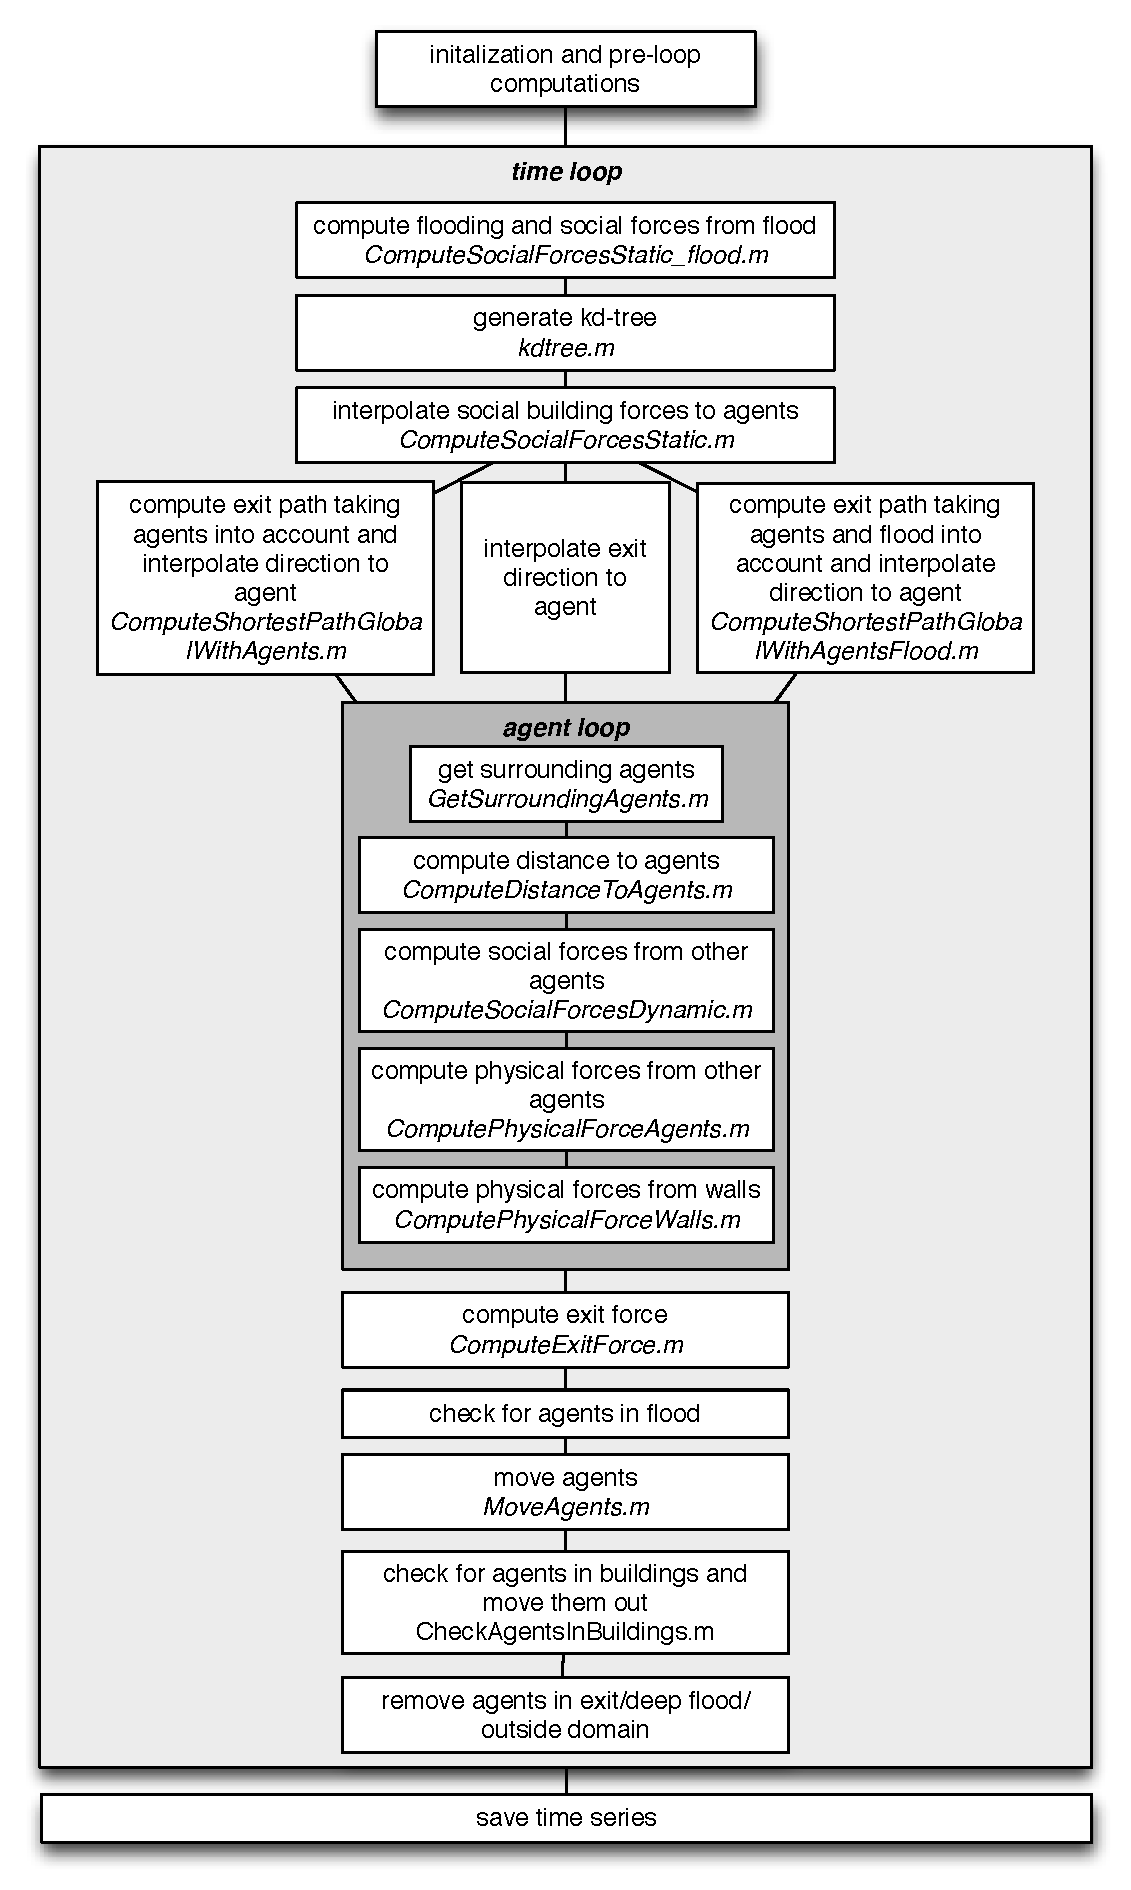
\includegraphics[height=0.8\textheight]{figures/EscapePanic}
\caption{Flow diagram of the main simulation function EscapePanic.m. Actions that are drawn in parallel belong to an if-loop.}
\label{fig:EscapePanic}
\end{figure}
To save computation time, we decided to compute several fields (e.g. the psychological forces from buildings) on a regular grid instead of computing it individually for each agent. To get the value of the respective field for an individual agent, we then interpolated this field to the agents. We assume that by using a sufficient high resolution (0.1 m spacing) for this field, our results are sufficiently accurate. The regular grid as well as the fields are computed before we enter the time loop in our simulations (also see fig.\ref{fig:pre-loop} for a flow diagram of the pre-loop computations). Additionally, we initalize an array of structures called AGENT, in which all values related to the agents are stored. This makes is relatively easy to access the parameters for each agent. The cost of using such an array is that the assignment of values to particular fields of a structure in the array is relatively expensive in terms of computational time since it is not straightforward to vectorize operations on such an array of structures. We therefore usually had to transfer the vlaues in the fields of the different structures to vector, perform the operation on this vector, then transferring it to a cell array, which then allowed us to assign the contents of this cell array to the respective field of the structures in the AGENT array of structures. However, since other operations take much more time in our simulation, we prefer this data structure because of its accessibility.\\
\begin{figure}
\centering
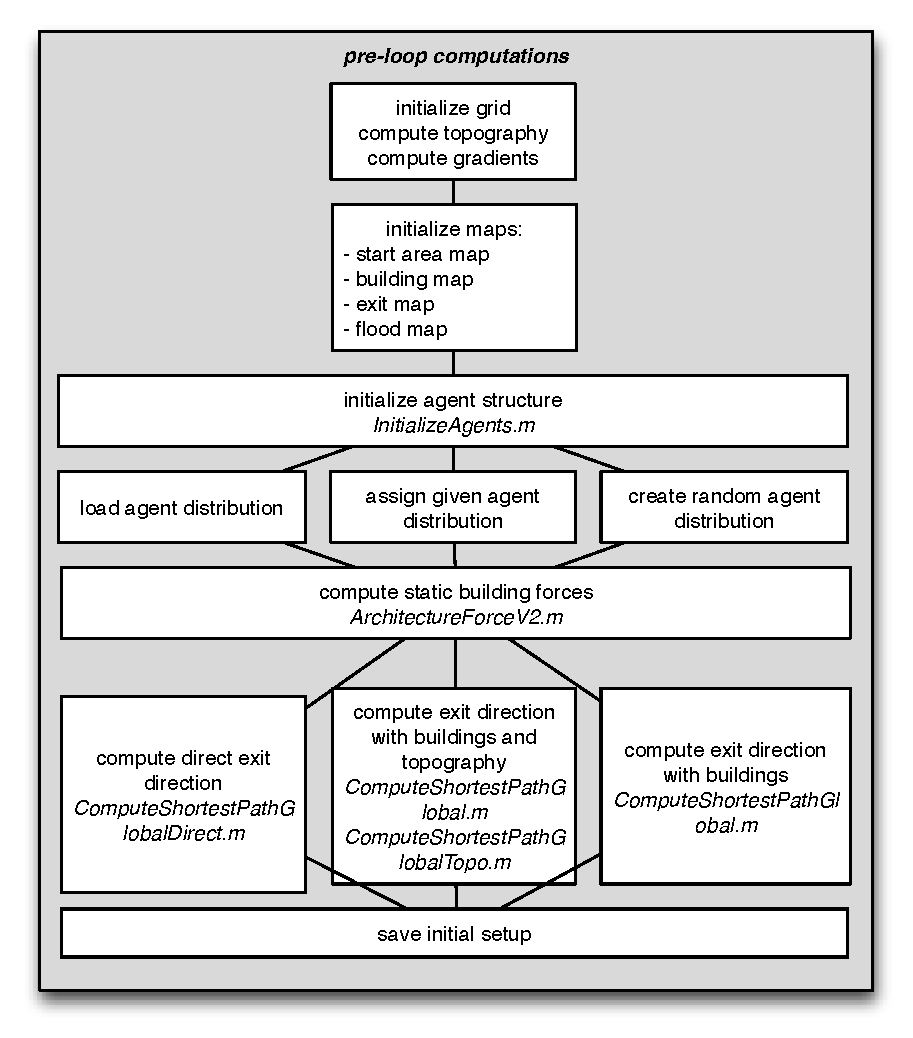
\includegraphics[height=0.5\textheight]{figures/PreLoopComputations}
\caption{Flow diagram of the pre-loop computations in EscapePanic.m. Actions that are drawn in parallel belong to an if-loop.}
\label{fig:pre-loop}
\end{figure}

\subsection{Initialization of Buildings, Exits and Flood maps}
Building information is passed to the EscapePanic function as a list where the minimal and maximal x- and y-values are stored. This is feasible only when using buildings that conform to the lines of a cartesian grid. In the case of more complex building structures, this would have to be changed. From this building list, we then produce a boolean building map with a high spatial resolution, where the nodes are assigned a 1 when a building is located at the respective node and 0 when no building is located there. This building map is then later on used in several functions. The same is done for exits and a flood map.
\subsection{Agents}
The AGENT structure is initialized using a separate function, where we initialize both agent parameters such as maximal agent velocity, mass etc. and fields that will contain information about forces acting on each agent later on. Several agent parameters can be varied in a random manner. The perturbation can be set in the input file by the user. Initial agent locations are computed in a random manner inside a predefined starting area.
\subsubsection{Agent forces}
The different forces acting on the agents are computed in different functions and stored in the AGENT array of structures.
\begin{description}
\item{\textbf{Psychological forces from buildings: }}As those forces are static throughout the simulation, they are computed before the time loop on a regular grid and then interpolated to the agents at each time step. Values that have to be interpolated are the magnitude of the force and the direction of the force. The direction is again normalized after interpolation. To compute the psychological forces on the regular grid, we use the MATLAB function bwdist from the image processing toolbox, which computes the distance from a node with value 0 to a node with value 1 in a very fast manner. 
\item{\textbf{Psychological forces from the flood: }}Those forces are computed in a similar manner as the psychological forces from the buildings, but as the water level is changing at each time step, this has to be done inside the time loop.
\item{\textbf{Psychological forces from agents: }}Prior to computing those forces, a kd-tree \citep{kdtree} is created inside the time loop to allow for a fast range search of the agent locations. Inside the agent loop, we then perform this range search to find all the agents located in a box around the "active" (meaning that the forces for this agent are computed in this step of the agent loop) agent. We then compute the distance of the active agent to the agents in this box and use this information to compute the social force resulting from those agents.
\item{\textbf{Physical forces from agents: }}Using the information about the distance from the step above, we can now compute the physical force from other agents acting on the active agent, if they are too close. We can compute both the normal as well as the tangential force. In our code, the tangential force computation lead to spurious effects, which is why we switched it off in our simulations. We suspect that there is a bug in this computation (most likely a sign error), but due to the limited amount of time available, we were not able to fix this issue.
\item{\textbf{Physical forces from buildings: }}The physical forces from building on the agent are also inly computed when the agent is getting too close to a building. As for the physical forces from the agents, we omit the tangential forces.
\item{\textbf{Exit forces: }}Exit forces can be computed in this code in two different ways: Either one can set the exit force to be proportional to the other social forces acting on the agent, only that the exit force is directed towards the exit, or one can use a constant exit force. We chose to use a constant exit force for simplicity. The computation of the exit direction is described below.
\end{description}

\subsubsection{Repulsive walls}
\label{sec:WallsImplementation}
Repulsive walls are added using a list of minimum and maximum values in x- and y-direction. Therefore only square buildings are implemented in the current version of the code. The single buildings are then put together into a building map, where we calculate the distance between every free point in the model domain (not covered by a building) and the nearest wall. From this distance we calculate the psychologic wall force on all agents and, if they touch the wall, the physical wall forces as well. Eq.~\eqref{eq:fiWS} for the psychologic wall force can be rewritten as

\begin{equation}
	{f_{iWS}} = \left\{ {{A_i} {\exp \left[ {\frac{{ - {d_{iW}}}}{{{B_i}}}} \right] \cdot \exp \left[ {\frac{{{r_i}}}{{{B_i}}}} \right]} } \right\}{{\bf n}_{iW}}
	\label{eq:fiWS2}
\end{equation}
which allows for calculating the first part already before starting the time loop. The second part is then added later on in the agent loop.

\subsubsection{Exit forces}
As mentioned above, we tested several different methodes to mimic the desire of an agent to reach the exit. All methods use a shortest path algorithm which was downloaded from the Matlab File Exchange \citep{fastmarching}. We then implemented 5 different ways to compute the desired direction to the exit of an agent:
\begin{description}
\item{\textbf{Direct exit direction: }}In this case, all nodes in our domain are assigned a constant velocity $v_0$, which is equal to the unperturbed maximal velocity of the agents. Using the fast marching algorithm, we then obtain the estimated time it takes to go from each node to the exit. Taking the gradient of this field in both x- and y-direction and normalizing them yields the desired direction of the agents.
\item{\textbf{Shortest path with buildings taken into account: }} In this case, we set the velocity at the nodes where a building is located to a very small value ($10^{-8}$). Setting this value to 0 results in numerical errors, since the travel time would then become infinite at those nodes. This approach also results in an exit direction that is perpendicular to the building walls at the nodes that are part of a building wall. This is actually desirable, as it adds an additional "desire" to the agent to stay away from a wall.
\item{\textbf{Shortest path with buildings and other agents taken into account: }} We implemented this extension by reducing the velocity at the nodes, where an agent is present, by a constant factor (which can be changed by the user). To do this, we had to loop over the agents and find the nodes that are inside their radius. We were not able to vectorize this part, which is why it takes up most of the time in our simulations. It would be desirable to find a way to speed up this part of the code. Taking agents into account sometimes resulted in unrealistic exit directions, which is why we decided to overly the shortest path field with agents taking into account with a field that was computed without agents. Those two fields can be weighted in an individual manner by the user.
\item{\textbf{Shortest path with buildings,other agents and topography taken into account: }}Including the topography effect in the shortest path computation proved to be a challenge, as the slope of the terrain changes with the walking direction. The problem, we had to solve is therefore strongly nonlinear. We first tried to iterate on the solution and gradually updating the solution in every iteration step, but this did not result in satisfying results, if the iterations converged at all. Therefore, we just took five iterations, since this was sufficient to compute the relevant features of the shortest path field. As the shortest path field with the agents is anyway added to this field, the details are not of such an importance.
\item{\textbf{Shortest path with buildings,other agents,topography and flood taken into account: }}In this case, we additionally set the velocity at the nodes which were flooded to a critical extent to a minimum value.
\end{description}

\subsection{Walking speed}
The implementation of the slope-dependent walking speed is relatively straight-forward. We assumed that the slope-dependency of the velocity only applies to the maximum velocity of an agent, therefore we only reduced its maximum velocity. We are aware that this is not entirely true, but as the agents usually reach their maximum velocity very fast, we assumed that our assumption is to first order accurate. To compute the slope of the terrain, we had to project the direction of the agent onto the gradient field in x- and y-direction (which was interpolated to the agent using linear interpolation). Using eq.\eqref{eq:walking_speed}, we then computed the maximum velocity and limited the velocity of the agent resulting from eq.\eqref{eq:vel} to this velocity.

\subsection{Flooding}

The flooding is similarly implemented as the repulsive walls described in Section~\ref{sec:WallsImplementation}. The top of the water level is repulsive by a magnitude lower value than those of the walls. Agents are allowed to cross this first waterfront, if they overcome this repulsive force. In the shallow water, the desired velocity ($v_0$) is reduced to half the value than on land. Agents might go deeper and deeper into the water until there is a second waterfront at a certain water depth level (0.2 m depth). This is also a repulsive front by the same value as walls this time. If agents still cross this front, they are subsequently removed from the model and sadly declared as drowned.

\subsection{Computational efficiency of the code}

The code is highly vectorized and pushed towards high efficiency in order to be able to model a very large area including many agents in an acceptable amount of time. Although it is not parallelized, it solves computationally expensive calculations in a relatively short time. We assume that inter-agent forces are only relevant in a certain range around the agent. This assumption is justified by the fact that pedestrians only have a limited range of sight in a crowd and that they tend to focus their attention on other pedestrians nearby. We therefore assume that only psychological forces from agents in a box with five meters edge length are relevant. To determine the number of agents inside that box, we make use of a very efficient kdtree implementation found on the Matlab File Exchange. The kdtree algorithm is an algorithm that allows for fast and efficient range searches, which is why we make use of it here.
Data visualization is done separately after computation. It actually takes more time than the computation itself. Since we do not need to visualize every timestep, we did not have a significant problem with this issue.

\section{Simulation Results and Discussion}

\subsection{Model setups}

In this study, we use a set of different model setups and several different model parameters. The model setups are i) room with one door, ii) a complicated path, iii) room with one door including topography, iv) a room with two doors and finally v) large beach setup with several buildings and topography where finally a flood is included. The different cases are listed together with their model parameters in Table~\ref{tab:Parameters}. Resolution test indicate the spatial resolution of $0.1$ m is sufficient and used throughout all the model setups. A constant time step of $0.01$ s turned out to be sufficiently small and is used in all the models.

%  \newpage  %TABLE parameters

\begin{landscape}
\begin{table}  
	% \centering
	 \begin{footnotesize}
	\caption{Models and numerical setups used in this work.}
	\label{tab:Parameters}
	\begin{tabular}{l l r r  r }
	\hline
	 \textbf{Model} & \textbf{Exit force} & \textbf{perturbations} & \textbf{topography} &\textbf{flood}  \\
	 & formulation & &  \\
	 & & &  \\
	\hline
		&  \\
			&   \\
	\hline
	{\bf Model1\_direct\_1}	& direct 	& no			& no& no	\\
	{\bf Model1\_direct\_2}	& direct 	& size, mass, $\Delta f_{ijS}$ 	& no& no\\
	{\bf Model2\_direct\_1}	& direct 	& size, mass 	& no 	& no\\
	{\bf Model2\_shortest\_1}	& sh. path & size, mass 	& no 	& no\\
	{\bf EscapePanicTwoExitsDirect} & direct & mass, $\Delta f_{ijS}$ & no& no\\
	{\bf EscapePanicTwoExitsShortestPath} & sh. path & mass, $\Delta f_{ijS}$ & no& no\\
	{\bf EscapePanicTwoExitsShortestPathAgent} & sh. path ag. & mass, $\Delta f_{ijS}$ & no& no\\
	{\bf EscapePanicTwoExitsShortestPathAgentTopo} & sh. path ag. top. & mass, $\Delta f_{ijS}$ & yes& no\\
	{\bf BeachRun5} & sh. path ag. top. & size, $v_0$, mass, $\Delta f_{ijS}$  & yes & yes\\
	{\bf BeachRun6} & sh. path ag. top. & size, $v_0$, mass, $\Delta f_{ijS}$  & yes  & yes\\
	{\bf BeachRun7} & sh. path ag. top. & size, $v_0$, mass, $\Delta f_{ijS}$  & yes  & yes\\
	{\bf BeachRun8} & sh. path ag. top. & size, $v_0$, mass, $\Delta f_{ijS}$ &  yes & yes\\
	\hline
	\end{tabular}
	
	{\bf sh. path:} shortest path formulation / {\bf sh. path ag.:} shortest path formulation with agents / {\bf sh. path ag. top.:}\\ shortest path formulation with agents and topography  \\
	\end{footnotesize}
\end{table}
\end{landscape}



\subsection{Simple evacuation bottleneck: One exit}

\subsubsection{Direct exit force}

\begin{figure}
	\begin{center}
	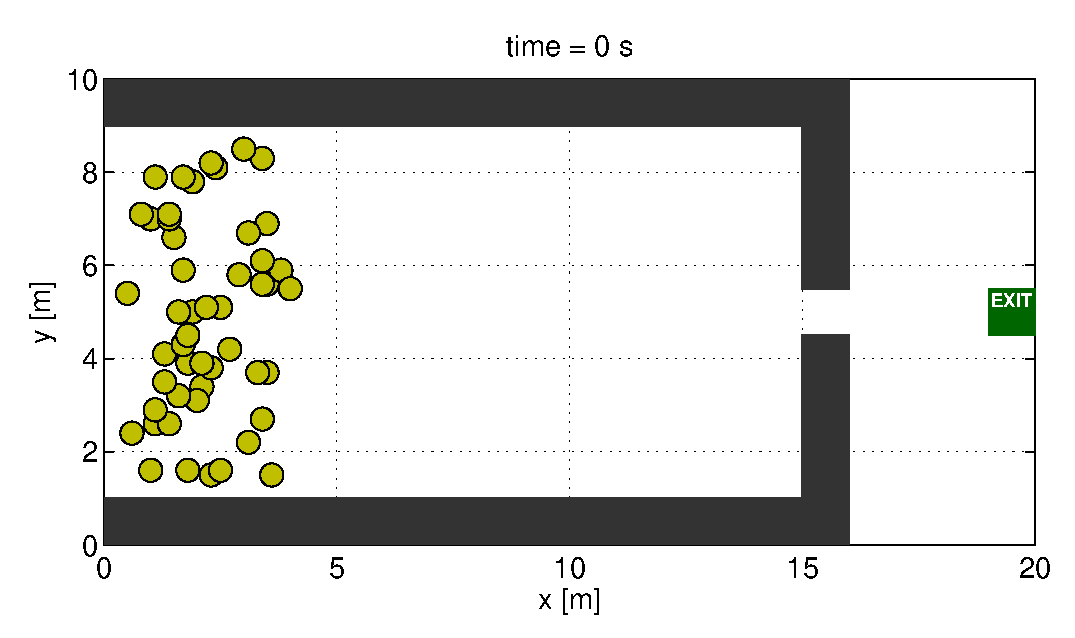
\includegraphics[width=0.6\textwidth]
	{figures/Model1_direct_1b_000000.eps}
	\qquad
	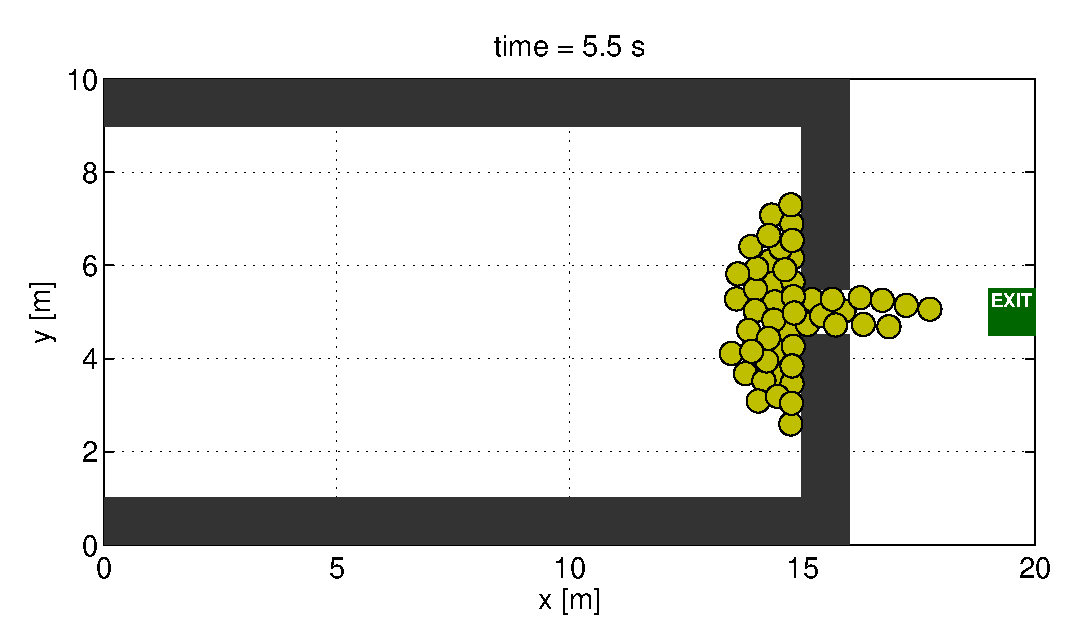
\includegraphics[width=0.6\textwidth]
	{figures/Model1_direct_1b_000550.eps}
	\qquad
	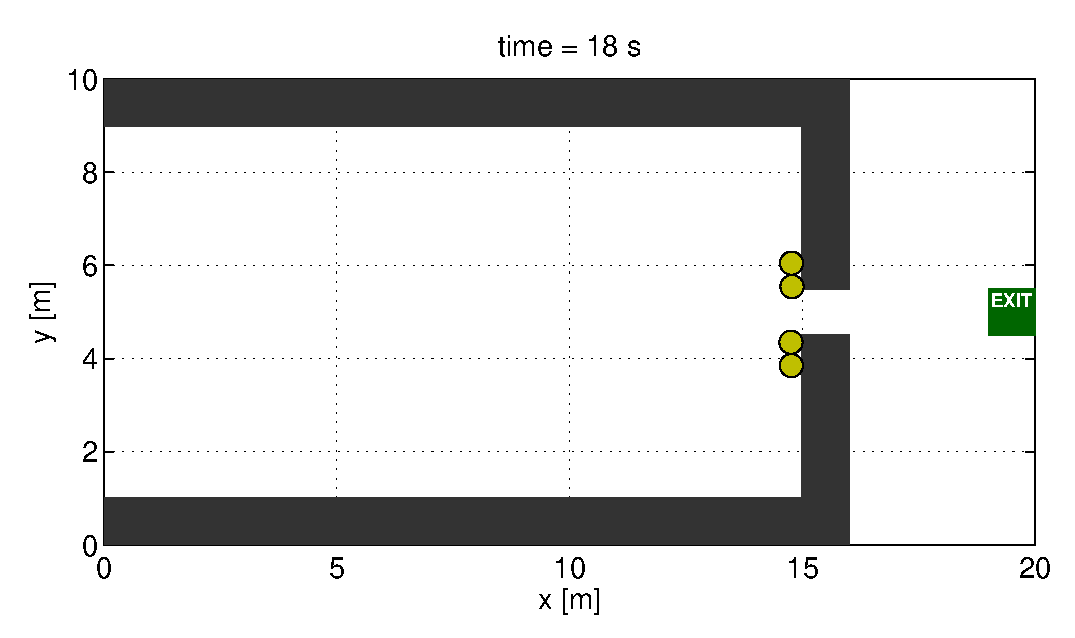
\includegraphics[width=0.6\textwidth]
	{figures/Model1_direct_1b_001800.eps}
	\caption{Time evolution of simple starting model for a room evacuation through a bottleneck. Initial setup (top), agents arriving at the bottleneck and accumulating in behind (middle) and agents blocking each other of exiting at the end of the simulation (bottom).}
	\label{fig:simple1}
	\end{center}
\end{figure}

The simplest version of our code has one exit (Fig.~\ref{fig:simple1}). The attractive force on the agents is defined to be linear towards the exit, thereby neglecting obstacles in between. The agents will not move towards an opening in an obstacle but toward the exit itself. Moreover, this formulation inhibits the agents of running around a bigger obstacle. This is a strong simplification but suitable to test the code. The behavior of the agents towards the repulsive walls and towards each other is satisfactory.

A first case ({\it Model1\_linear\_1}) is shown in Fig.~\ref{fig:simple1}. The model setup consists of a $15\times9$ m room that is bounded by repulsive walls. A $1\times1$ m door is the only exit thereof and leads to the attractive main exit of the model. The agents are initially placed randomly in an $3.5\times7$ m area in the left hand side of the domain (Fig.~\ref{fig:simple1}b). The model is not satisfactory, because at the late stage of evacuation there are two agents opposite of each other preventing them to exit the room (Fig.~\ref{fig:simple1}c). The counter parting psychologic social forces cancel all other forces out and therefore both agents remain at their position.

\begin{figure}
	\begin{center}
	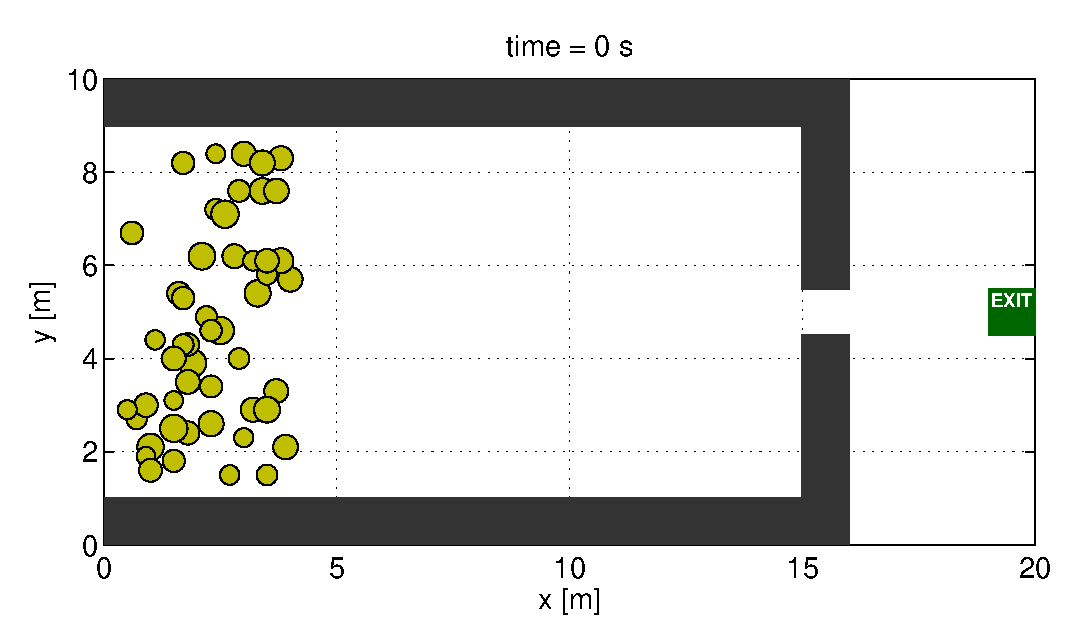
\includegraphics[width=0.6\textwidth]
	{figures/Model1_direct_2b_000000.eps}
	\qquad
	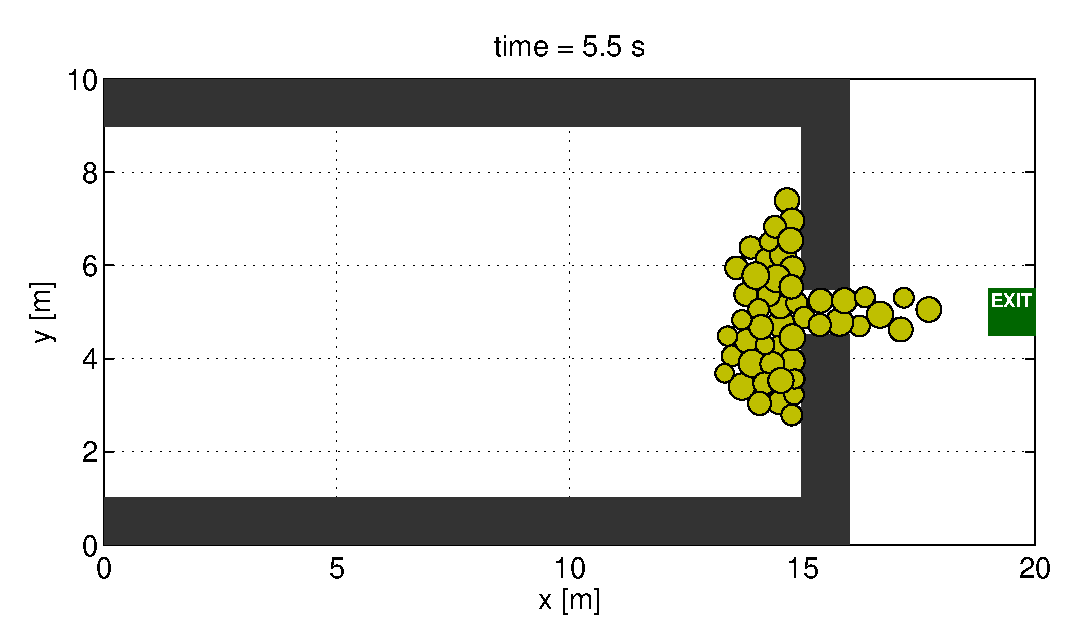
\includegraphics[width=0.6\textwidth]
	{figures/Model1_direct_2b_000550.eps}
	\qquad
	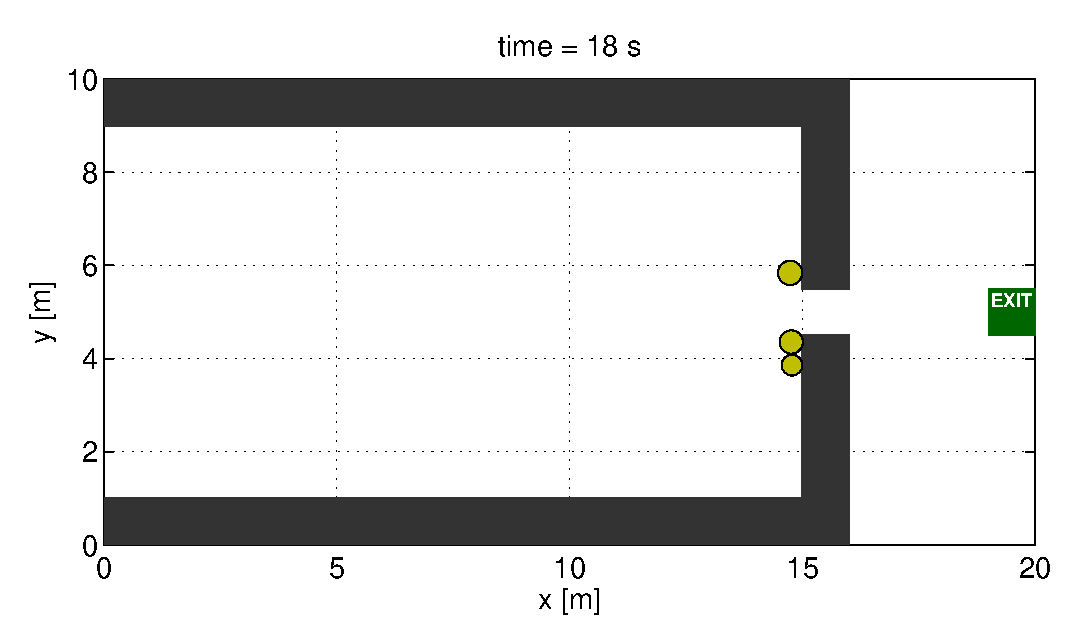
\includegraphics[width=0.6\textwidth]
	{figures/Model1_direct_2b_001800.eps}
	\caption{Time evolution of model including perturbations for a room evacuation through a bottleneck. Initial setup (top), agents arriving at the bottleneck and accumulating in behind (middle) and agents blocking each other of exiting at the end of the simulation (bottom).}
	\label{fig:simple2}
	\end{center}
\end{figure}

In order to introduce some noise into an otherwise perfect model we added several perturbations ({\it Model1\_linear\_2}). The psychologic social force between the agents is perturbed by a random small value in the order of $\pm 0.05$ N. Another complexity is added by characterizing the different agents. Accounting for different appetite and/or stomach behavior, their mass is randomly chosen with a perturbation of $\pm 10$ kg. A bigger radius is subsequently needed for fulfilling mass conservation. Therefore the agent's radius is randomly perturbed by $\pm 0.05$ m. The results of these adjustments are shown in Fig.~\ref{fig:simple2}.

Still the last two pedestrians are disabled of leaving the room because of the counteracting forces they exert on each other. This shows, that the "perfectness" of the model was not the main problem of this occurrence. The main cause of it might be found in the way the attractive exit force is described. The agents are pulled with the exit force directly towards the position of the exit, neglecting possible obstacles in between. Hence, in the case of the two blocked pedestrians, the main force is directed perpendicular to the wall instead of tangential to the wall towards the wall door. The force in this direction is very small and can thus easily be overweighted by the repulsive social force of the opposite agent. The agent is kept at his current position.

A solution of this problem therefore might be found in a different description of the attractive exit force by e.g. using a shortest path formulation.

\subsubsection{Shortest path formulation}

The shortest path formulation as described in Section~\ref{sec:Exits1} can improve the nature-like behavior of the model dramatically. A new setup is chosen to illustrate this and shown in Fig.~\ref{fig:simple3} and~\ref{fig:simple4}.

\begin{figure}
	\begin{center}
	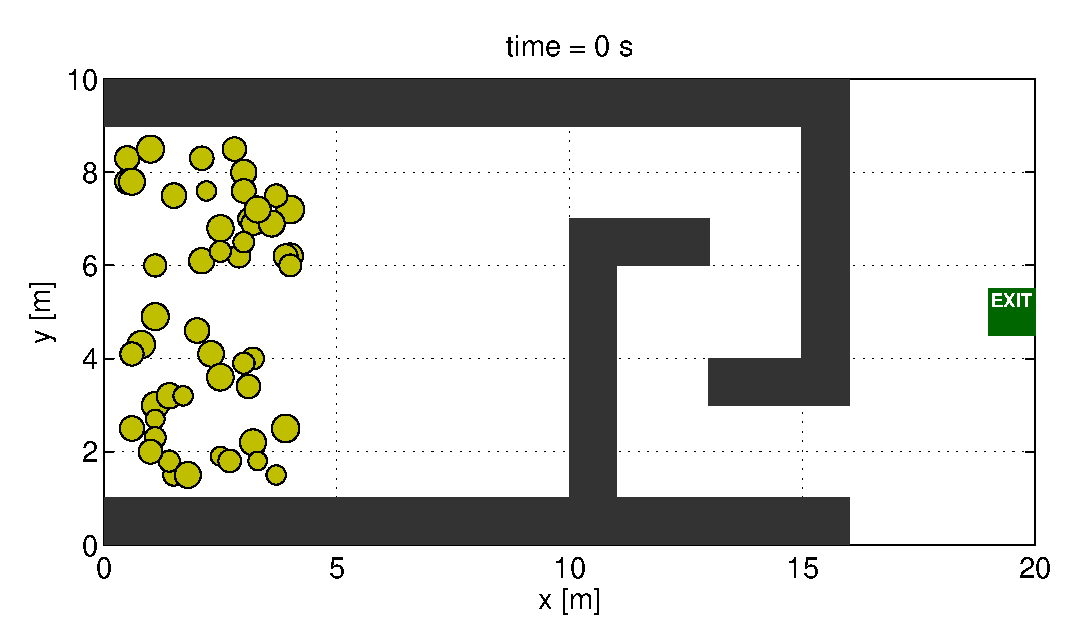
\includegraphics[width=0.6\textwidth]
	{figures/Model2_direct_1b_000000.eps}
	\qquad
	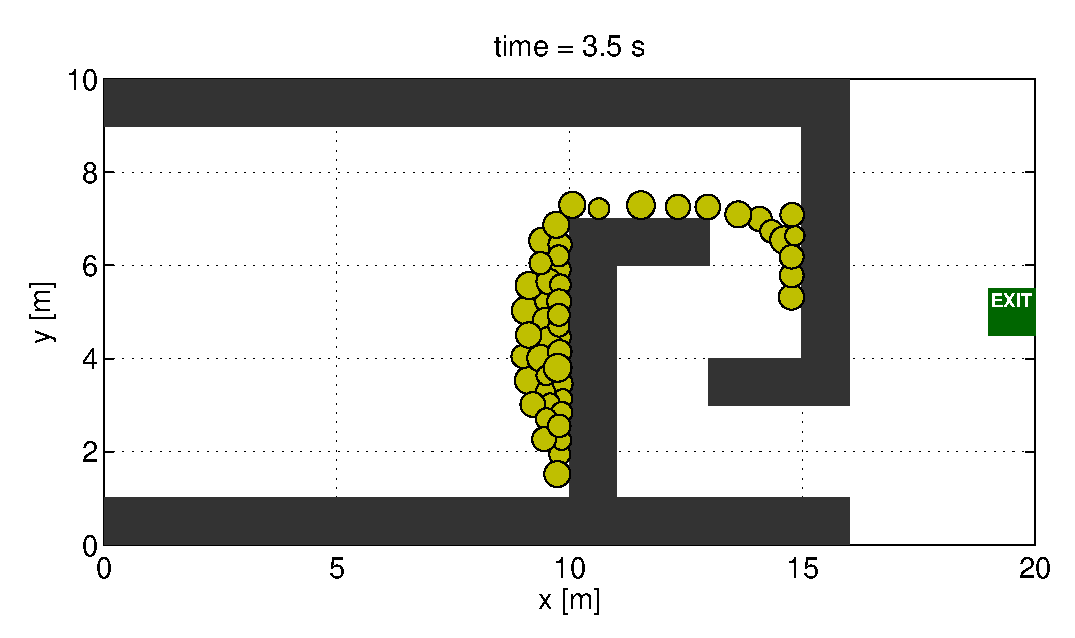
\includegraphics[width=0.6\textwidth]
	{figures/Model2_direct_1b_000350.eps}
	\qquad
	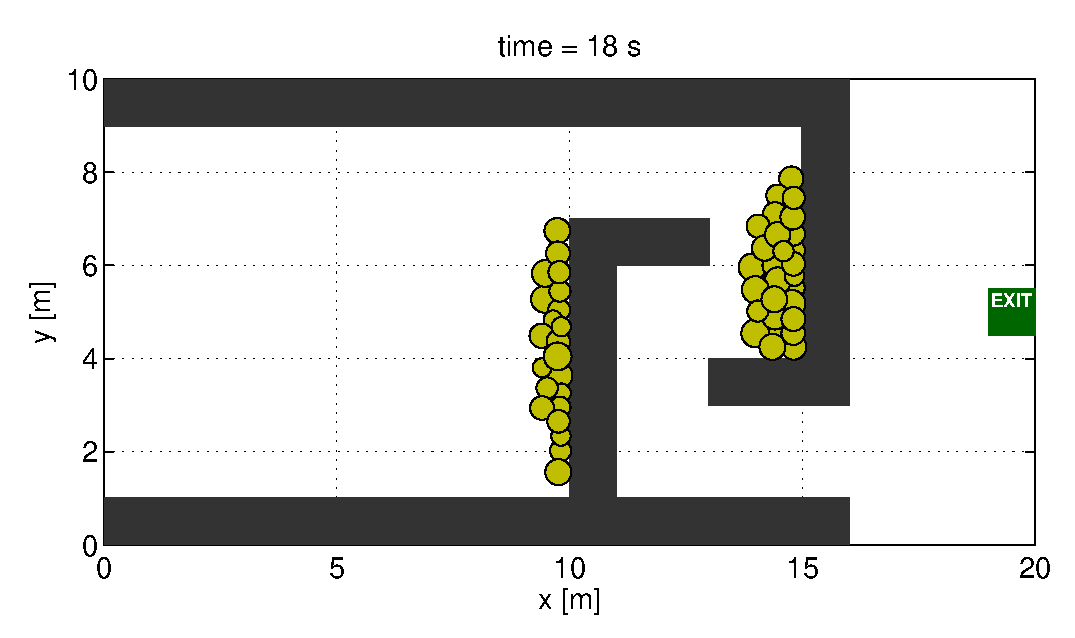
\includegraphics[width=0.6\textwidth]
	{figures/Model2_direct_1b_001800.eps}
	\caption{Time evolution of model with direct exit force formulation for a pedestrian flow around complicated architecture. Initial setup (top), agents arriving at the barrier walls and accumulating  (middle) and agents getting stuck and not able to move around an obstacle at the end of the simulation (bottom).}
	\label{fig:simple3}
	\end{center}
\end{figure}

The walls are placed in a way that the pedestrians have to move around corners and even away from the exit to finally arrive there. This is not straight forward and a simple exit force formulation is not able to describe the pedestrian flow in such a case (Fig.~\ref{fig:simple3}). The Agents get captured by obstacles with no direct passage towards the exit and are not able to leave such a place. 

The more elaborated shortest path formulation, on the other hand, can describe such a more complicated pedestrian flow in a realistic manner (Fig.~\ref{fig:simple4}). The agents are able to see all possible passages towards an exit in the whole model and are therefore able to choose the fastest way.

\begin{figure}
	\begin{center}
	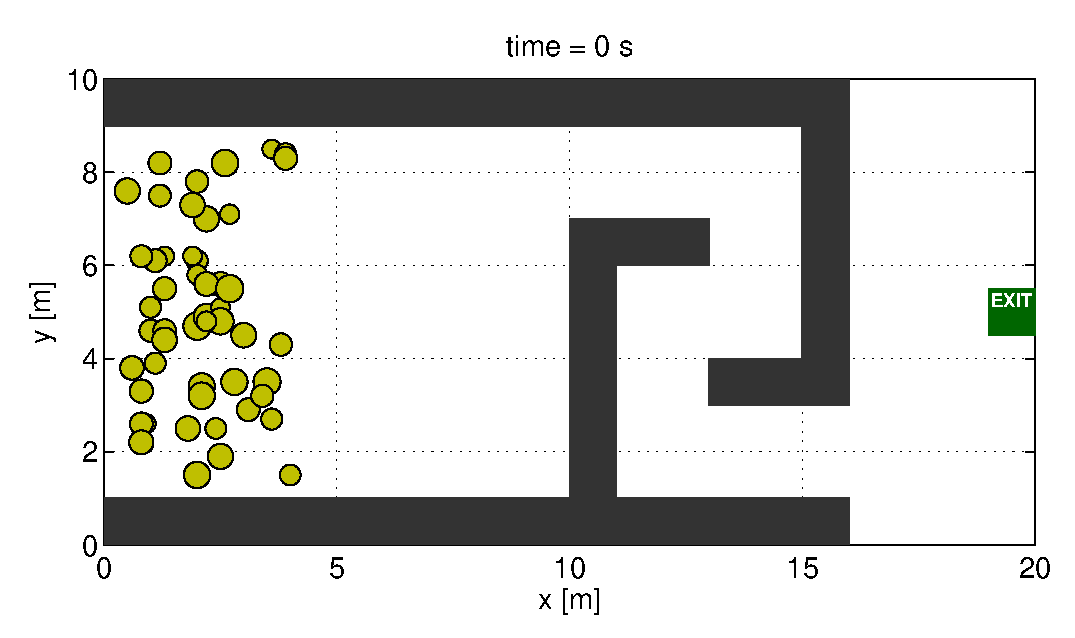
\includegraphics[width=0.6\textwidth]
	{figures/Model2_fastest_1_000000.eps}
	\qquad
	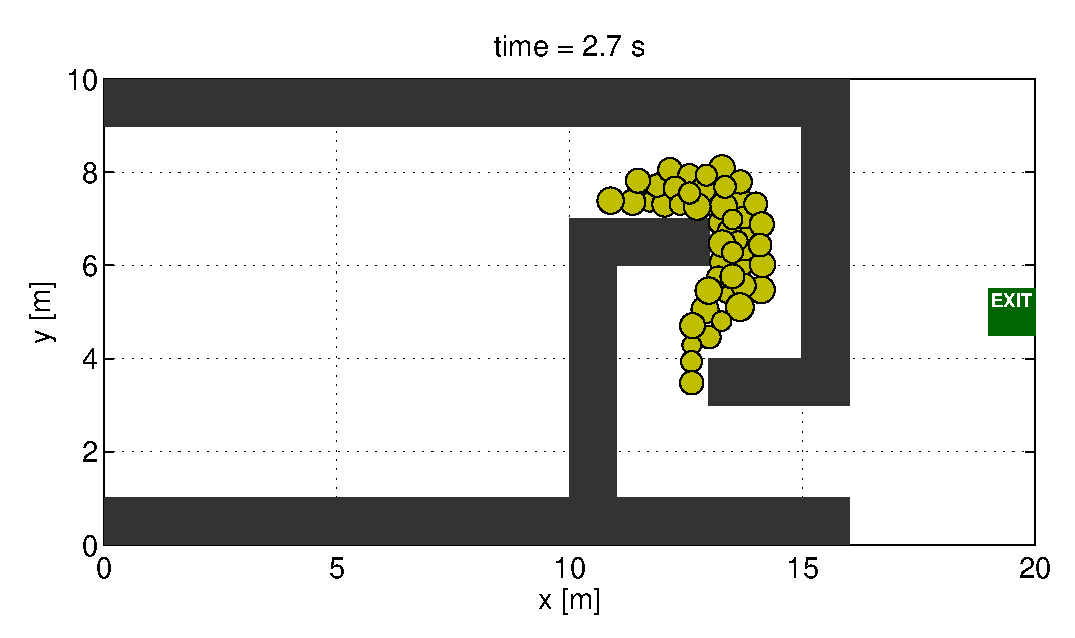
\includegraphics[width=0.6\textwidth]
	{figures/Model2_fastest_1_000270.eps}
	\qquad
	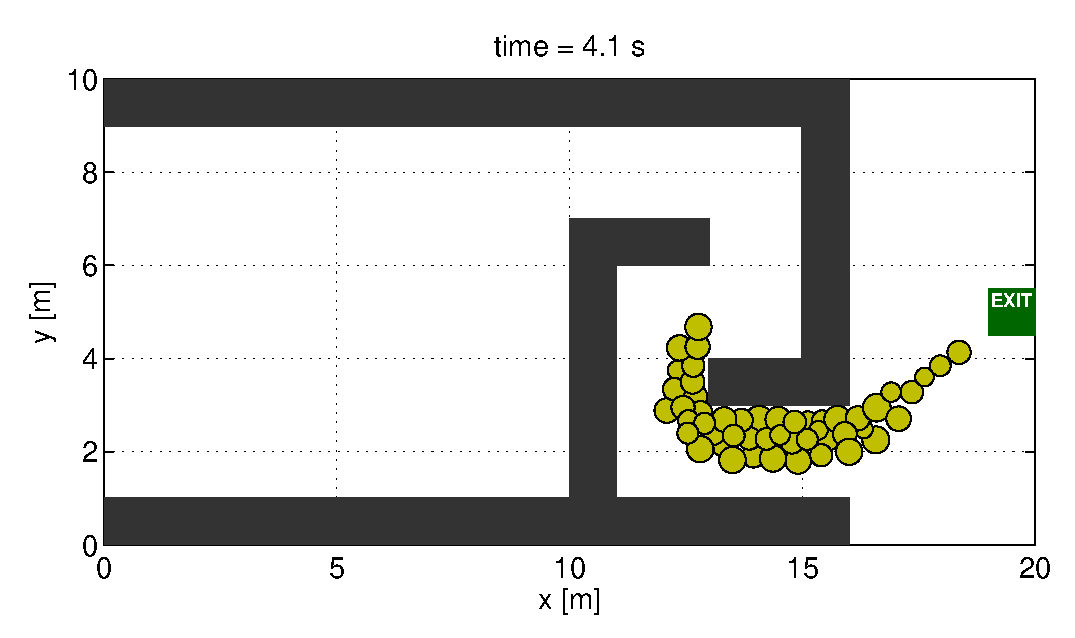
\includegraphics[width=0.6\textwidth]
	{figures/Model2_fastest_1_000410.eps}
	\caption{Time evolution of model including shortest path formulation for a pedestrian flow around complicated architecture. Initial setup (top), agents moving closely around corners (middle) and agents able to move around obstacles in the fastest way and arriving the exit at the end of the simulation (bottom).}
	\label{fig:simple4}
	\end{center}
\end{figure}

\subsection{Simple evacuation bottleneck: Two exits}

As we saw in the one-exit models, the shortest path formalism led to a more realistic behaviour of the agents. In a second step, we now extended the model by introducing one additional exit, leaving out the additional obstacles. In a first step, we used the shortest path procedure to determine the desired direction of the agent. As this did not lead to the desired agent behaviour (see Section~\ref{sec:two_exits1}), we had to extend the shortest path procedure by additionally taking agents into account (the procedure is described in Section~\ref{sec:implementation}). This led to a significant improvement in agent behaviour. As we additionally have to deal with topography in our model, we then introduced a small topography in our model to assess its effect on agent behaviour. In the three following subsection, we shortly show and discuss the results of the different setups.

\subsubsection{Shortest path exit force}\label{sec:two_exits1}

Here, the exit direction of the agents is given by the shortest path algorithm, which has proven to yield better results compared to the direct path approach. Instead of having one gap in the wall as before, we now have two gaps in the wall. Additionally, the exit was switched slightly towards the lower gap. This makes the lower gap more preferable, since the path to the exit through this gap is shorter.

As one can see in Fig.~\ref{fig:two_exits1}, the shortest path algorithm results in a rather unrealistic behaviour of the agents: Instead of opting for the upper gap in case the lower gap is blocked by other agents, all agents choose the lower gap.

\begin{figure}
	\centering
	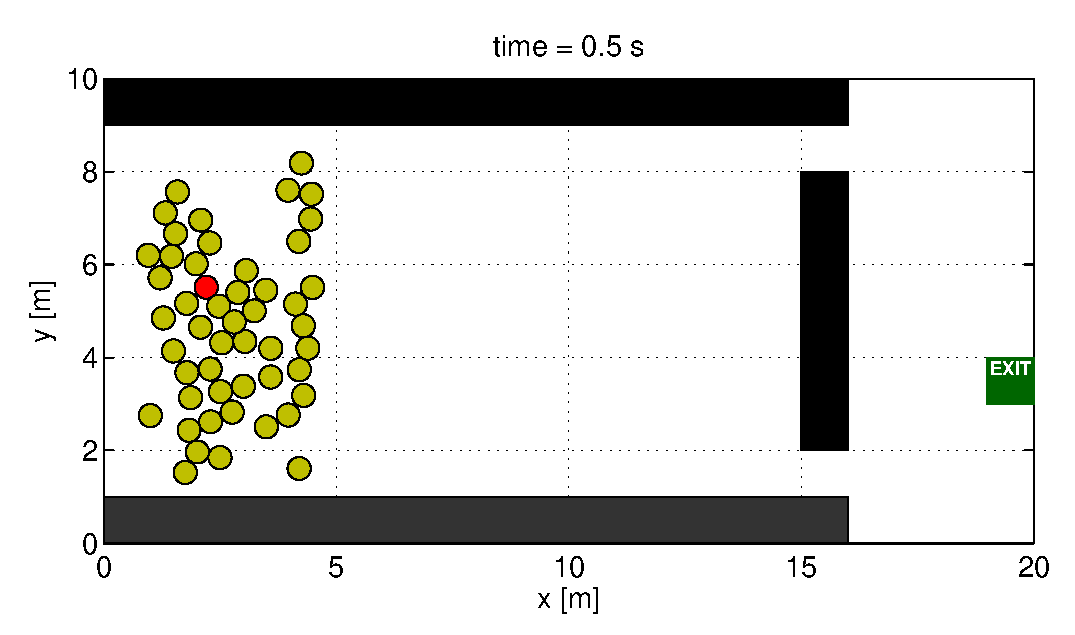
\includegraphics[width=0.6\textwidth]{figures/TwoExitsShortestPath_000050.eps}
	\qquad
	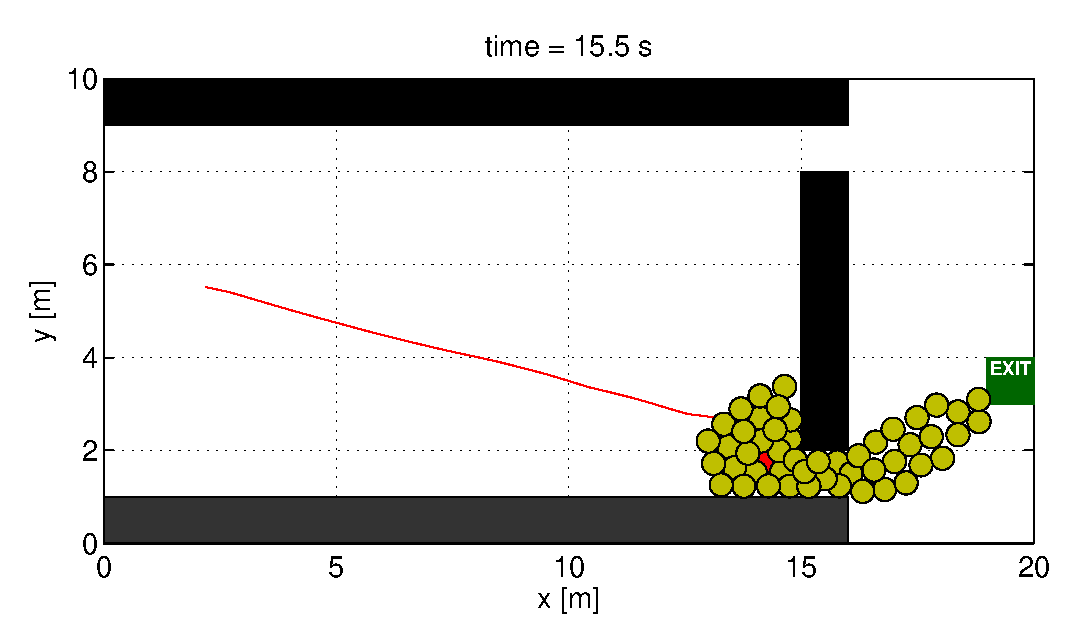
\includegraphics[width=0.6\textwidth]{figures/TwoExitsShortestPath_001550.eps}
	\qquad
	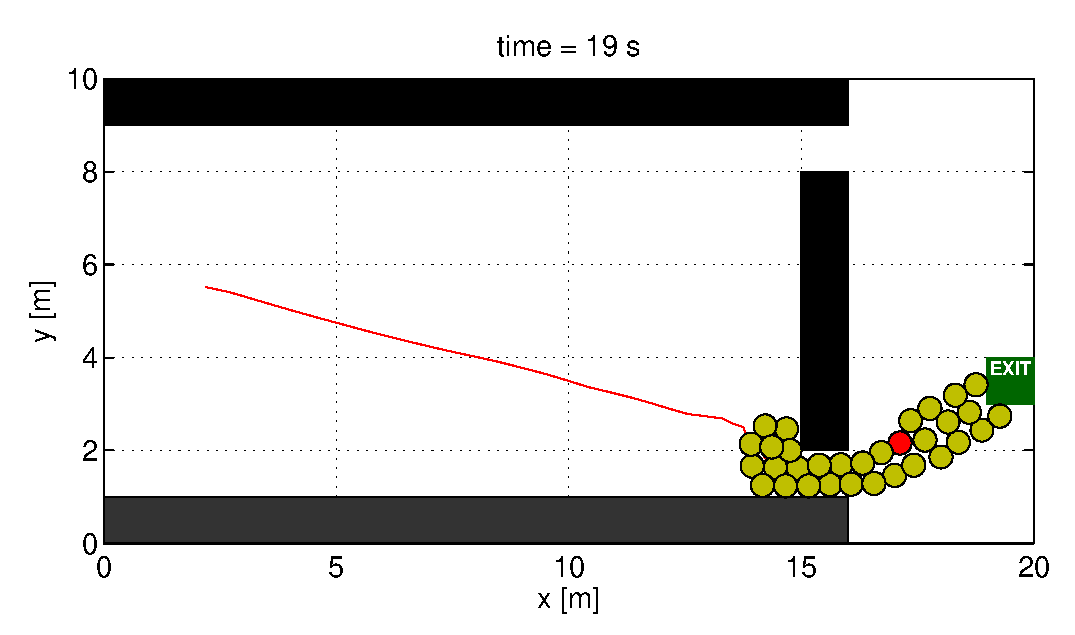
\includegraphics[width=0.6\textwidth]{figures/TwoExitsShortestPath_001900.eps}
	\caption{Snapshots of the time evolution of a simple two-exit model using the shortest path algorithm to determine the exit direction. As can be seen, the simple shortest path formalism doesn't work in a realistic manner, since all the agents opt for the closest exit regardless of other agents blocking the way. For a better illustration, we chose one agent (named Don) and plot his path through the model domain. As one can see, Don never changes his direction on the way to the exit.}
	\label{fig:two_exits1}
\end{figure}

This behaviour is clearly not what one could observe in reality, since at least some agents would prefer the upper gap and reach the exit significantly faster than in our simulation. We therefore had to adjust the shortest path procedure to account for agents blocking the way.
\subsubsection{Shortest path exit force with agents taken into account}
In the second simulation, we used the extended shortest path procedure to determine the exit direction of the agents. We tried different combinations of the sensitivity of the agents to other agents blocking the way. The (in our opinion) best results were obtained when we reduced the estimated velocity at a node by a factor of 2.5. In Fig.~\ref{fig:two_exits2}, it can be seen that the behaviour of the agents is much more realistic than before. In this simulation, agents frequently re-decide on the path to be taken and change from the lower to the upper gap or vice versa if either of those gaps is blocked.

\begin{figure}
	\centering
	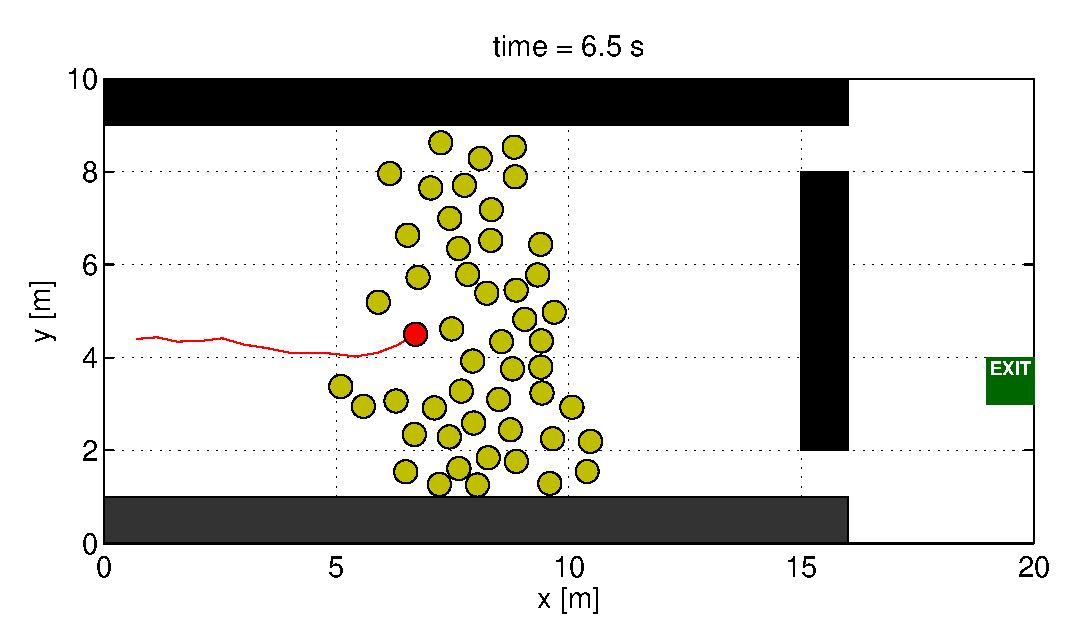
\includegraphics[width=0.6\textwidth]{figures/TwoExitsShortestPathWithAgents_000650.eps}
	\qquad
	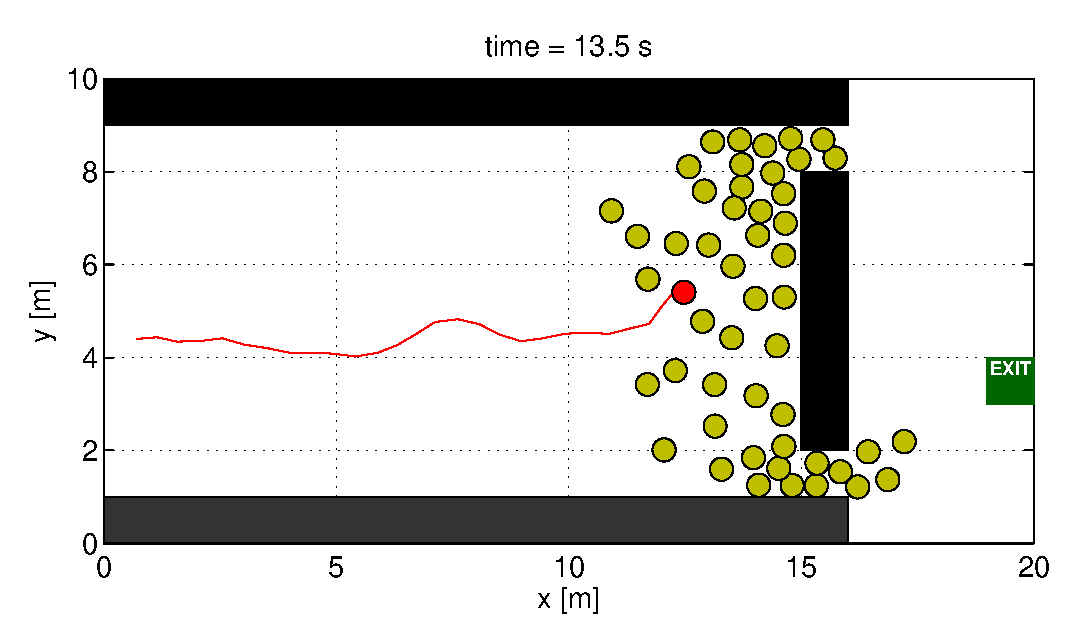
\includegraphics[width=0.6\textwidth]{figures/TwoExitsShortestPathWithAgents_001350.eps}
	\qquad
	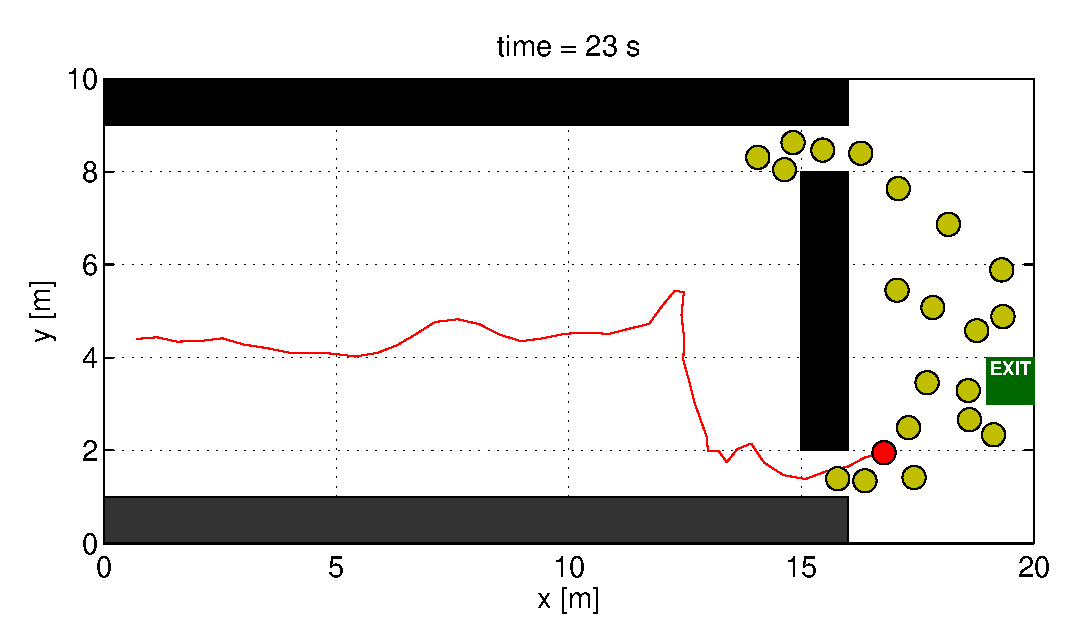
\includegraphics[width=0.6\textwidth]{figures/TwoExitsShortestPathWithAgents_002300.eps}
	\caption{Snapshots of the time evolution of a simple two-exit model using the shortest path algorithm to determine the exit direction. In this case, agents blocking the way to the exit are taken into account. This enables the agents to redecide on the path taken to the exit depending on the agent density in between. The path of our example agent Don clearly shows this process. At first, Don chooses a path that keeps him in between both exits due to the agents in front of him. Then, as crowding at the lower exit occurs, he decides to go towards the upper exit, but then redecides as the lower exit becomes less crowded again.}
	\label{fig:two_exits2}
\end{figure}

\subsubsection{Shortest path exit force with agents and topography taken into account}

In this last simulation, we tested the influence of topography on agent behaviour. For this reason, we introduced a slight topography in our model. The topography is essentially a two-dimensional Gaussian curve, which is given by the equation:

\begin{equation}
	z(x,y) = A\exp \left(- \frac{\left(x-x_0\right)^2}{2\sigma_x} + \frac{\left(y-y_0\right)^2}{2\sigma_y}\right)
\end{equation}

In this simulation, we chose $A = 1 $ m, $x_0 = 10$ m, $y_0 = 5$ m, $\sigma_x = 15$ m and $\sigma_y = 6$ m.

\subsection{Evacuation of a beach in the case of a tsunami event}

\begin{figure}
	\centering
	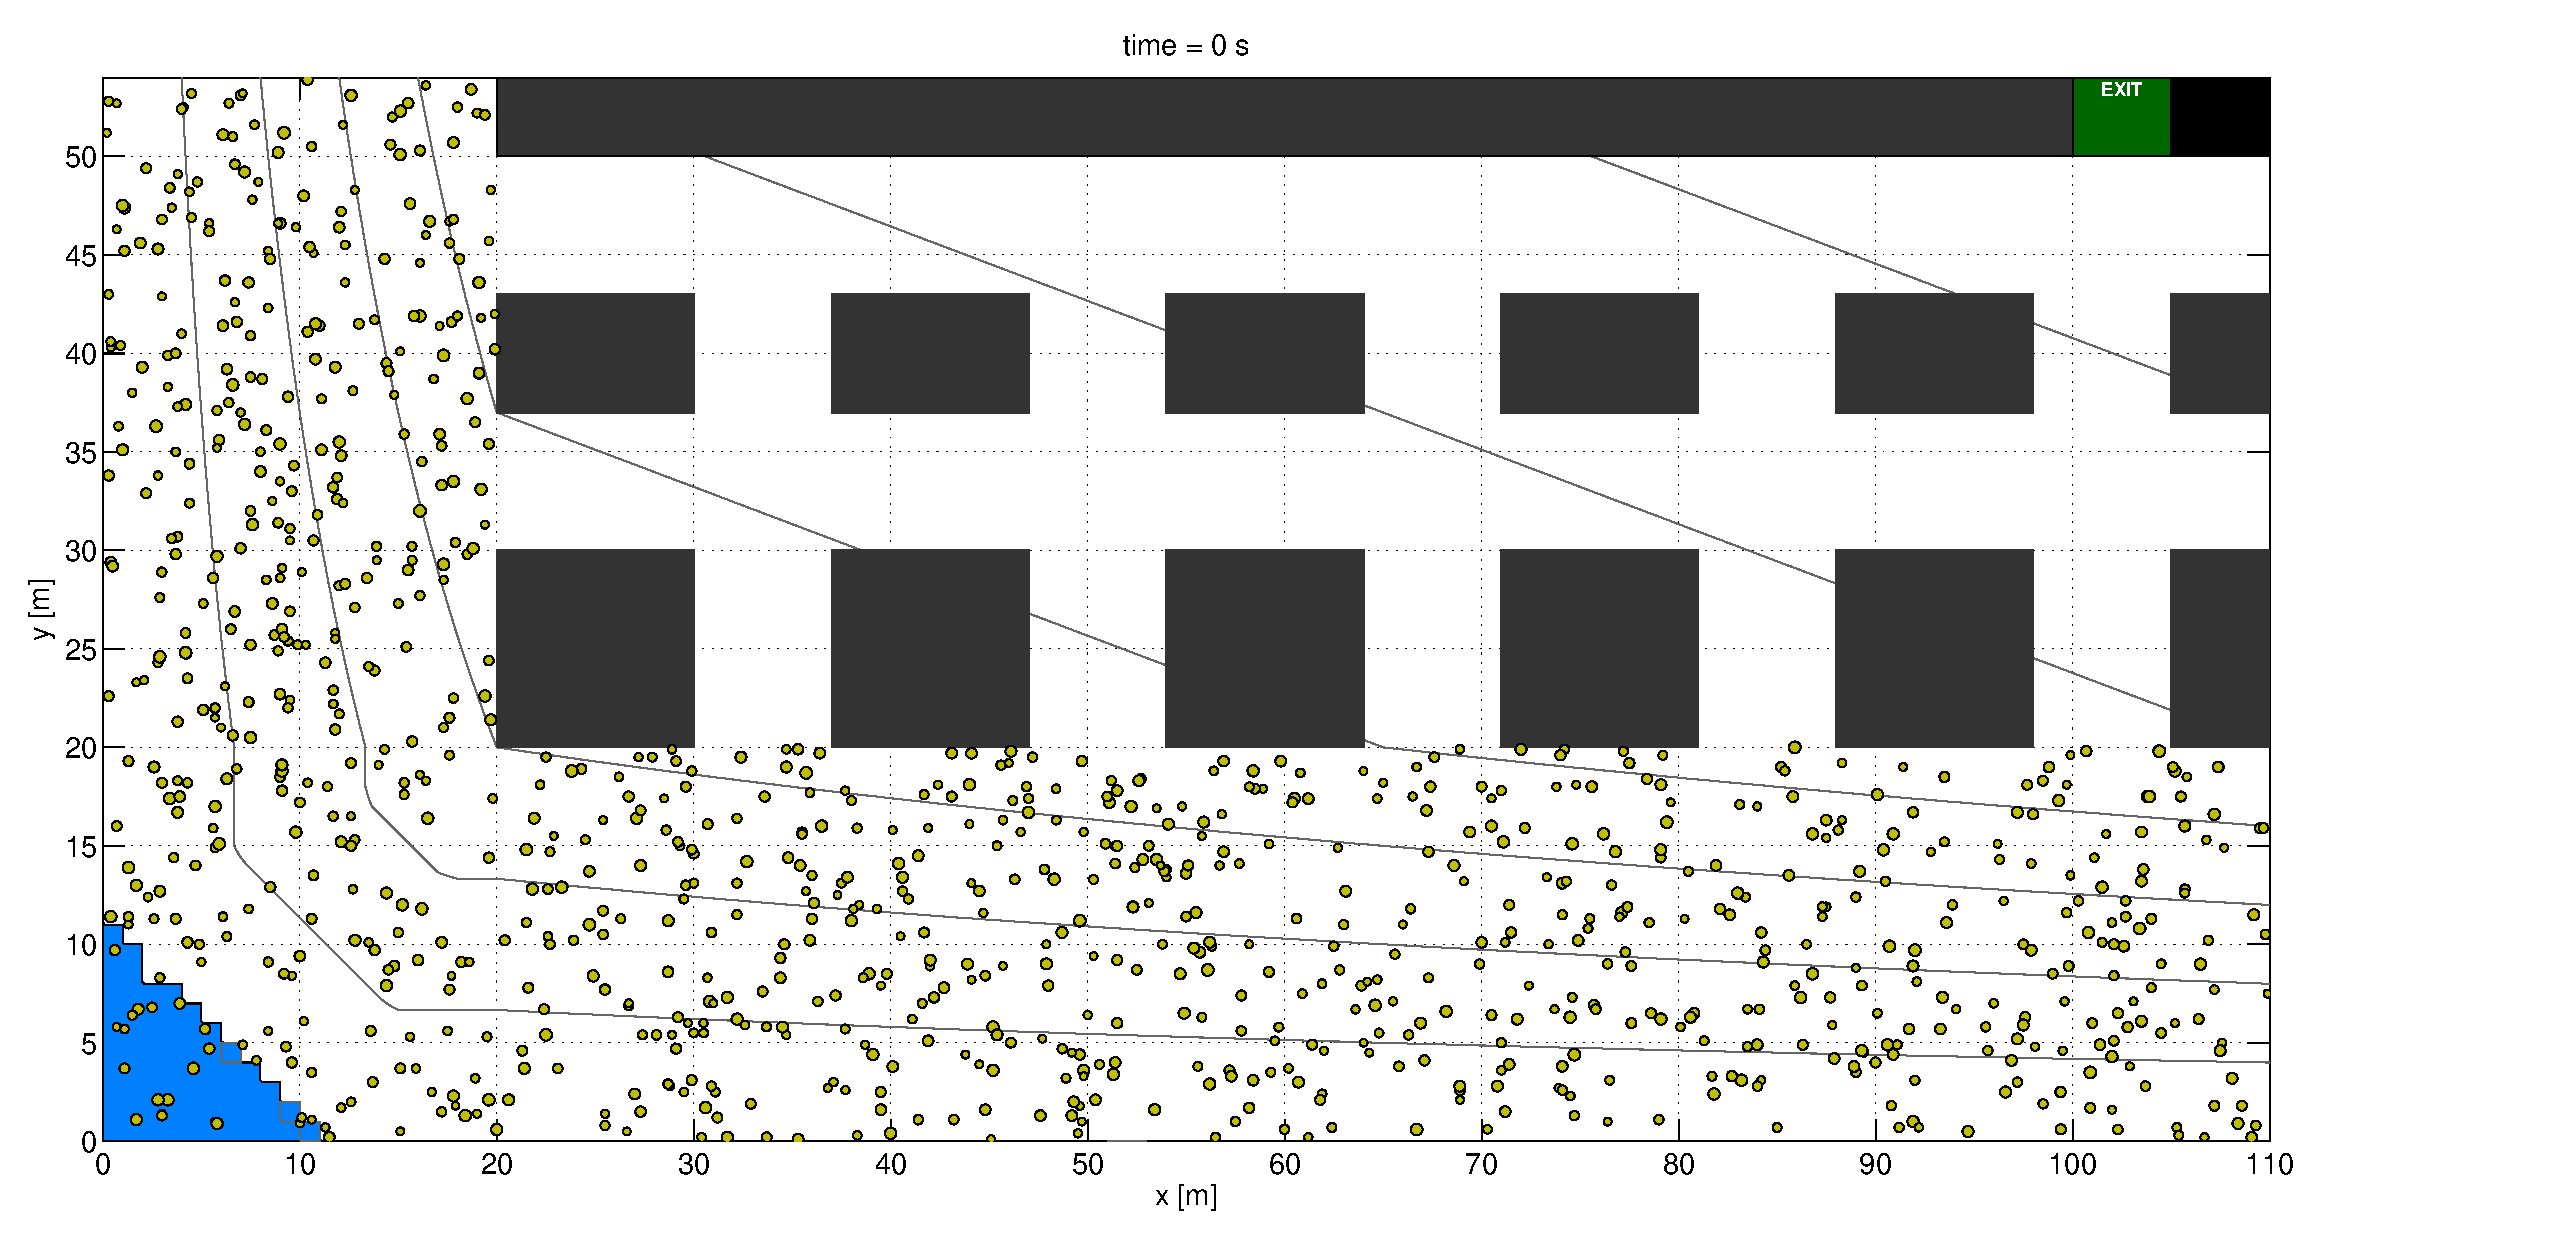
\includegraphics[width=1.1\textwidth]{figures/BeachEvacuationOneExitStreetWidth7_Flood0_1_000000.eps}
		\qquad
	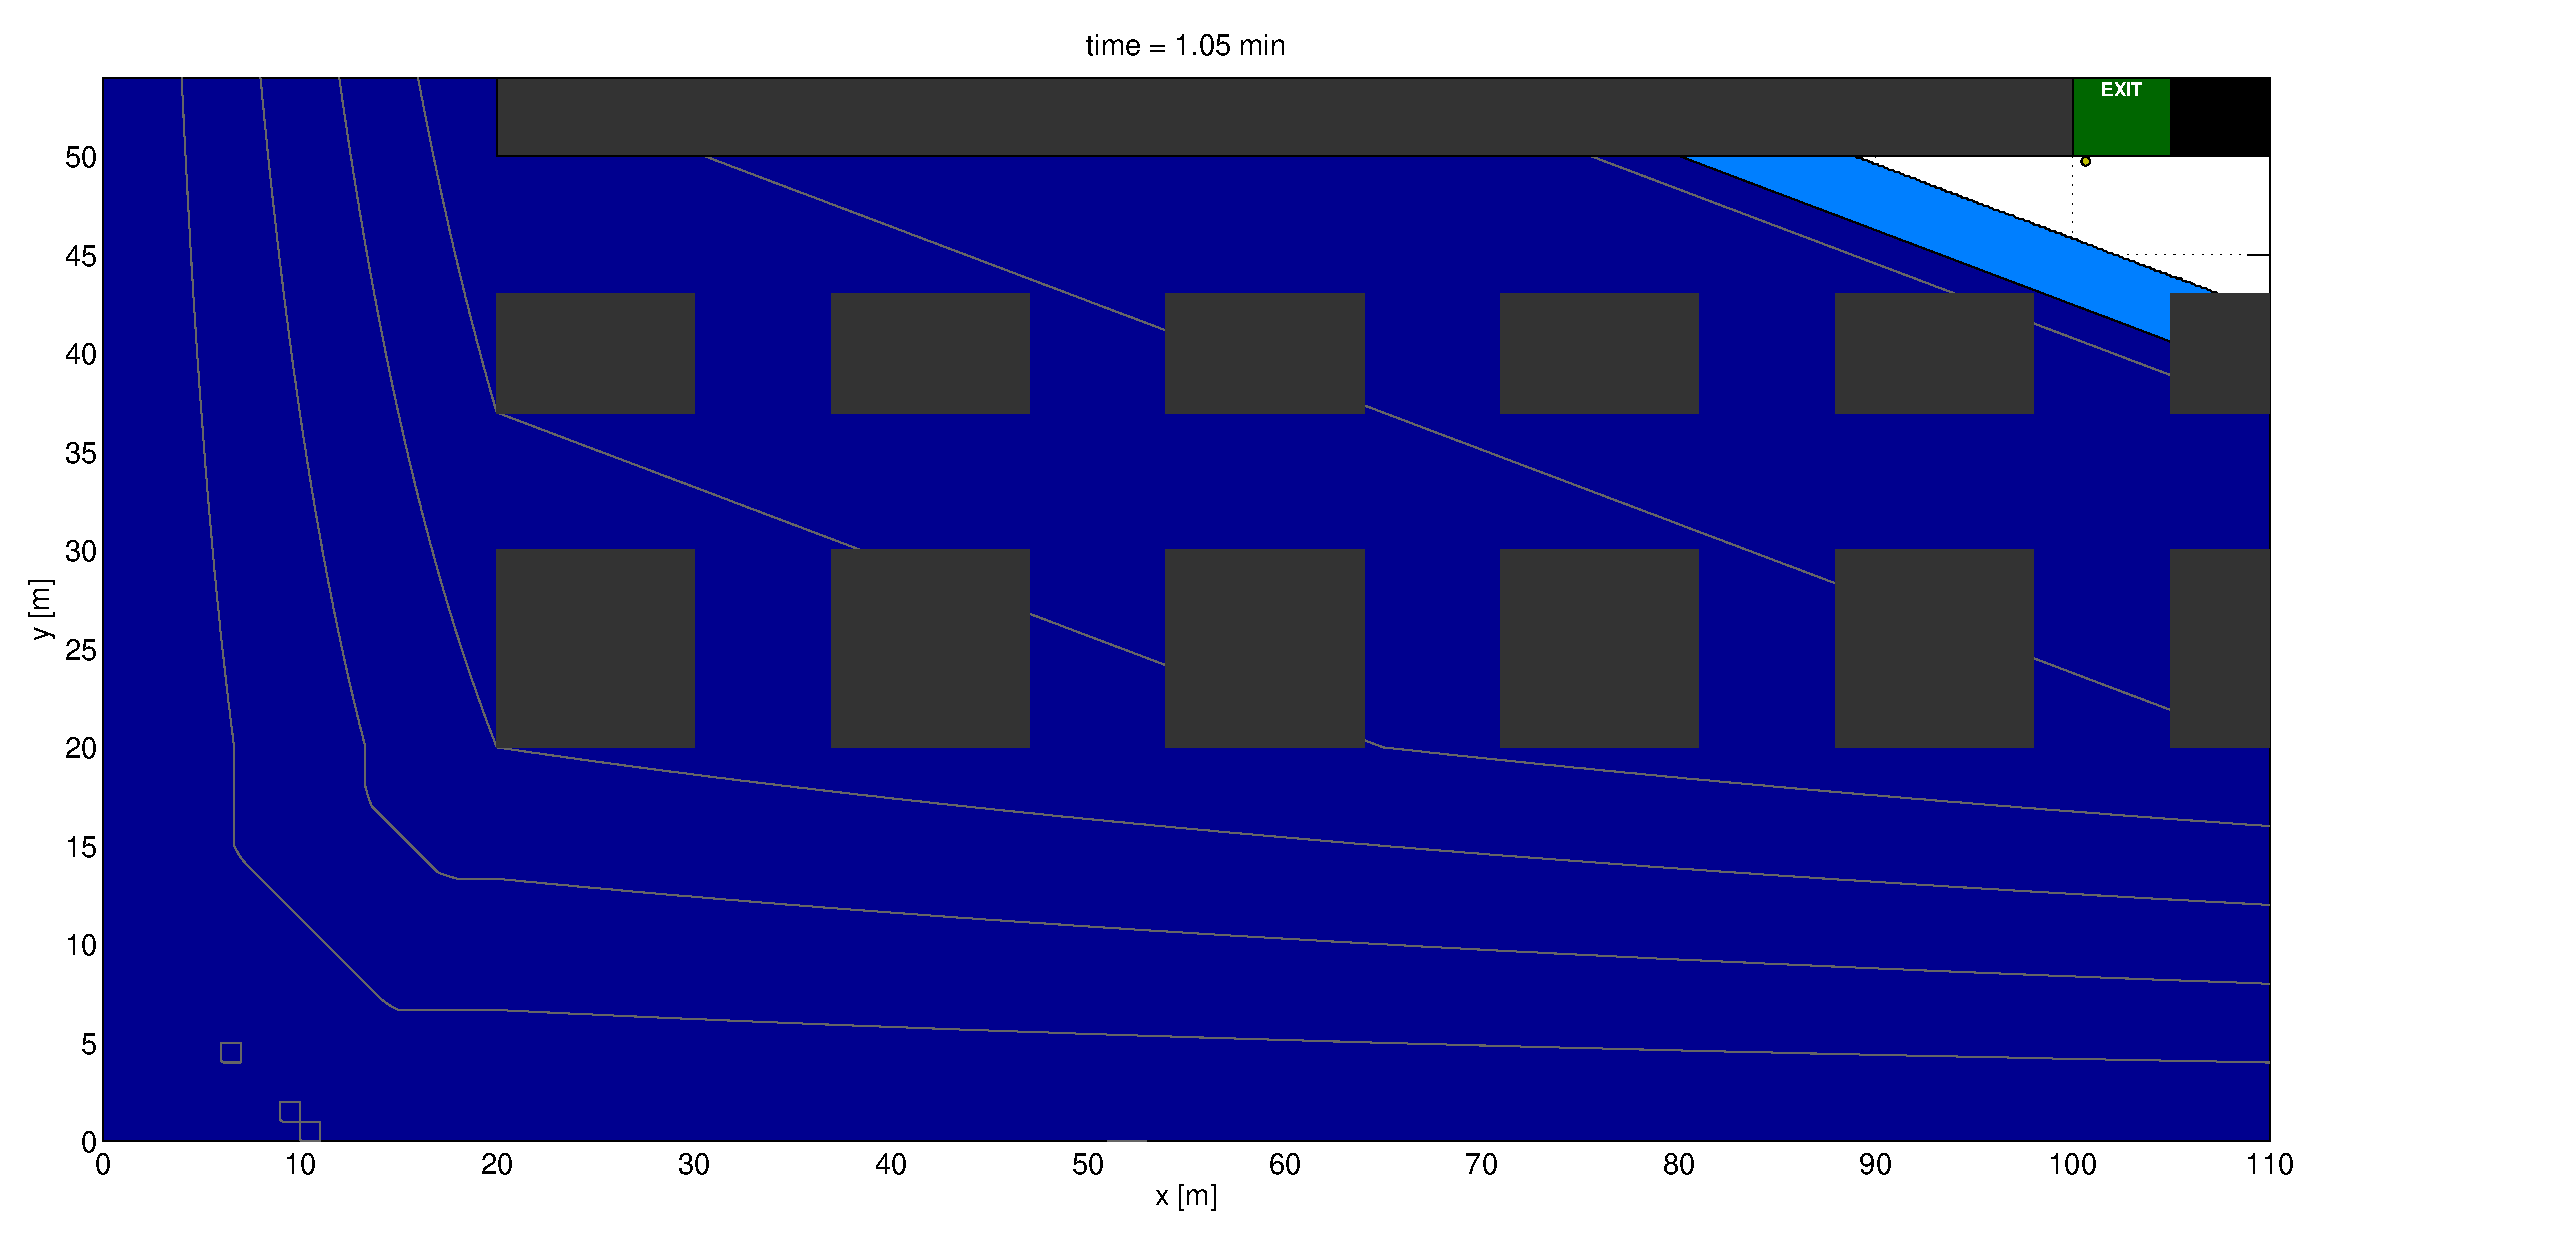
\includegraphics[width=1.1\textwidth]{figures/BeachEvacuationOneExitStreetWidth7_Flood0_1_006300.eps}
	\caption{Initial condition of the beach evacuation model: 1000 pedestrians (yellow circles) swimming or lying in the sun (top). Final stage of evacuation model: last surviving pedestrian arrives at exit just before the flood reaches him. Black squares indicating beach houses or anti-flood wall, green square is the exit, grey contours indicating topography and blue contour indicates water covered surface for shallow (cyan) and deep water (dark blue), respectively.}
	\label{fig:beach_initial}
\end{figure}

Fig.~\ref{fig:beach_initial} shows the initial model setup that consists of $55\times110$ m wide box, several beach houses and a anti-flood wall in the back including a relatively wide exit. Topography is included in this setup shown by the topography contours. This is needed for a flood to rise over time until the water reaches the only exit of the model. One thousand people are initially placed at the beach close to the water (or in the water). At the model start, the flood starts to rise and the people immediately start to panically escape the beach area towards the exit. The beach houses in between hinder them (depending on the model setup) to do so in a sufficiently short time. The goal of this setup is to evaluate the escape possibilities from the beach depending on the width of the streets between each house parcel. Therefore we here present four different models using different parcel spacings.

\begin{figure}
	\centering
	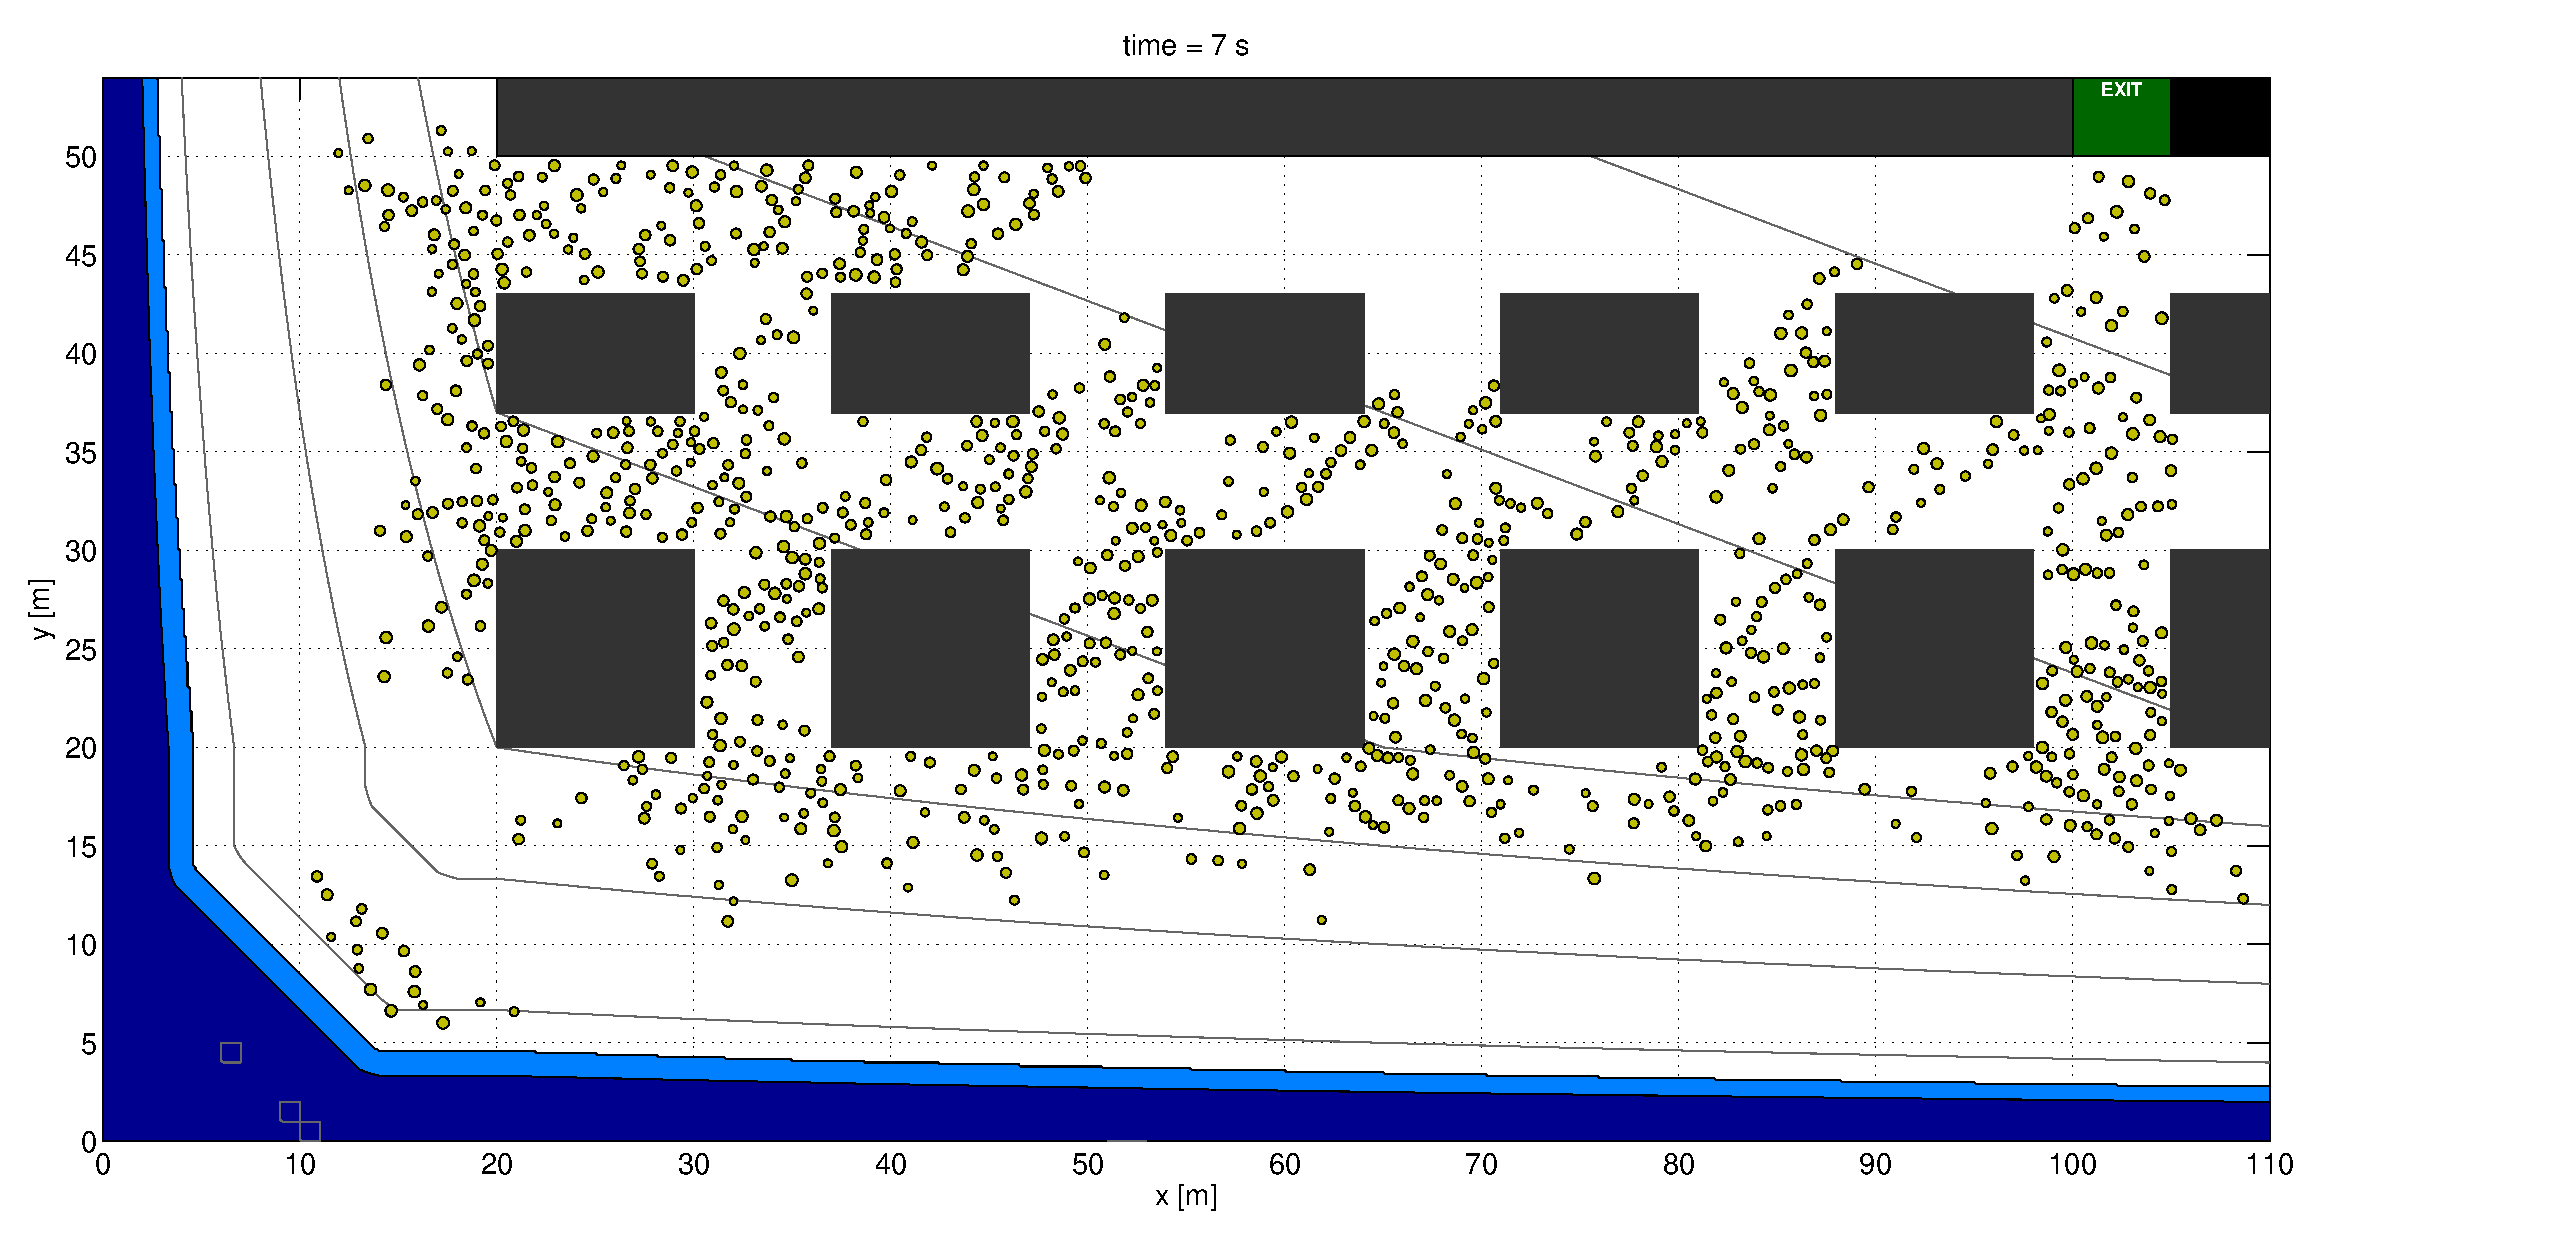
\includegraphics[width=1.1\textwidth]{figures/BeachEvacuationOneExitStreetWidth7_Flood0_1_000700.eps}
	\qquad
	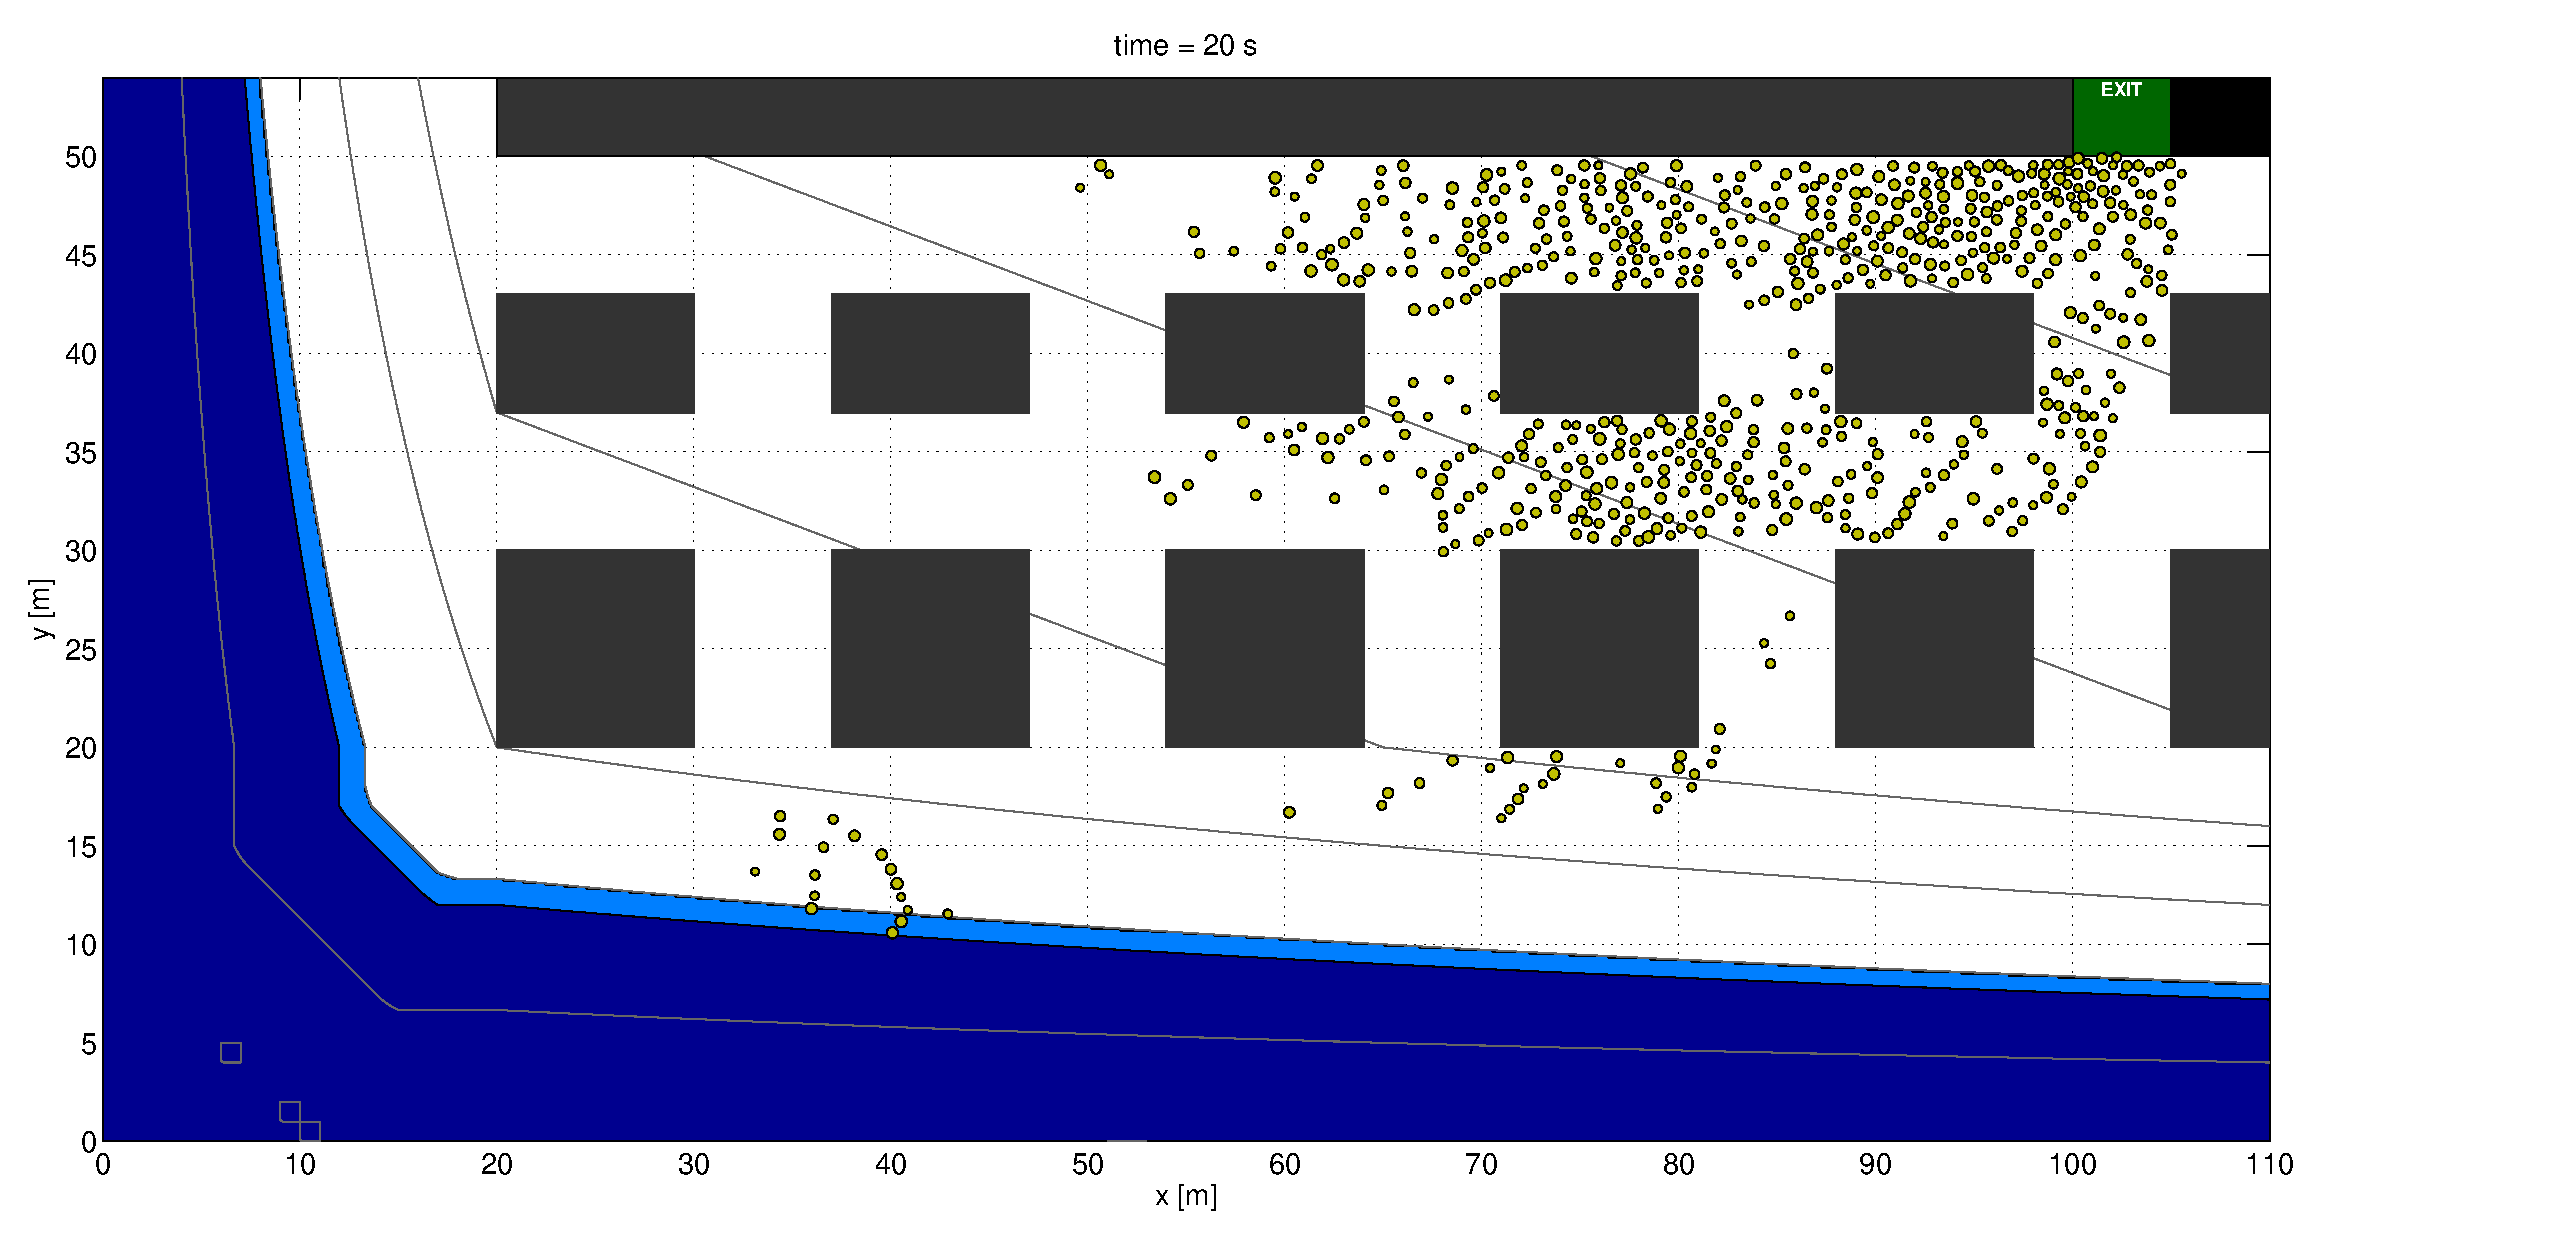
\includegraphics[width=1.1\textwidth]{figures/BeachEvacuationOneExitStreetWidth7_Flood0_1_002000.eps}
	\caption{Wide beach house setup: different time steps show the approach of the flood and the escaping pedestrians.}
	\label{fig:beach_1}
\end{figure}

Fig.~\ref{fig:beach_1} shows the model evolution using a wide parcel spacing of 7 m. In this experiment, pedestrians do not have problems in escaping the rising flood: Their escape path is very easy and thus also sufficiently short. People do not accumulate to much, because there are no dramatic bottlenecks.

\begin{figure}
	\centering
	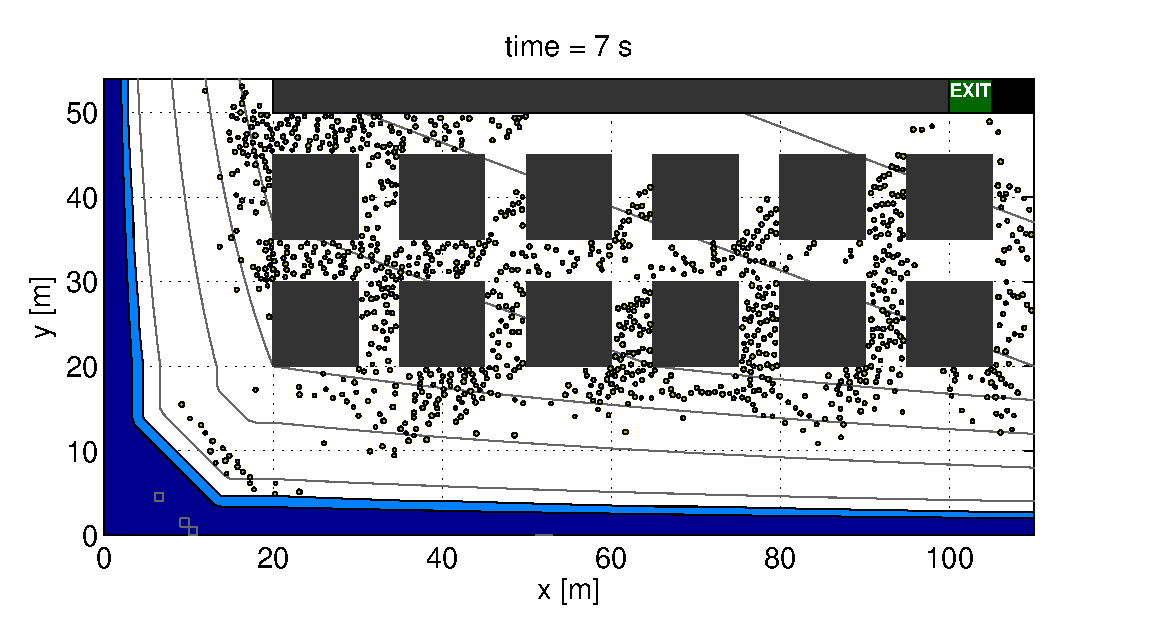
\includegraphics[width=1.1\textwidth]{figures/BeachEvacuationOneExitStreetWidth5_Flood0_1_000700.eps}
	\qquad
	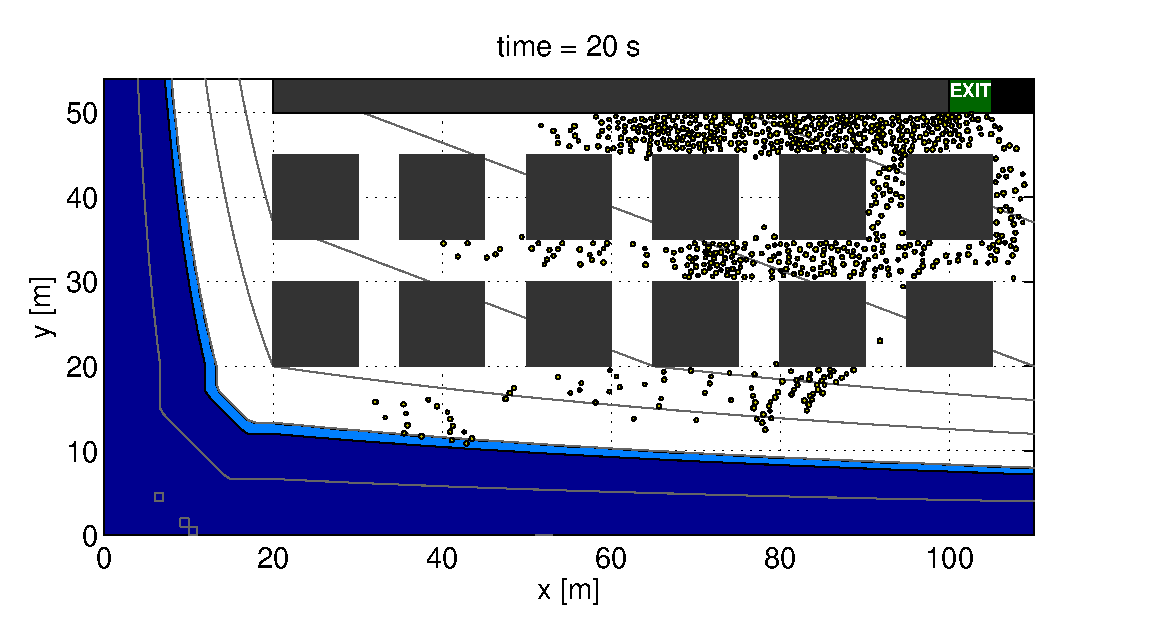
\includegraphics[width=1.1\textwidth]{figures/BeachEvacuationOneExitStreetWidth5_Flood0_1_002000.eps}
	\caption{Intermediate beach house setup: different time steps show the approach of the flood and the escaping pedestrians.}
	\label{fig:beach_2}
\end{figure}

A slightly denser setup is shown in Fig.~\ref{fig:beach_2}. The spacing between two adjacent parcels is here 5 m wide. People again seem to be able to escape well.

\begin{figure}
	\centering
	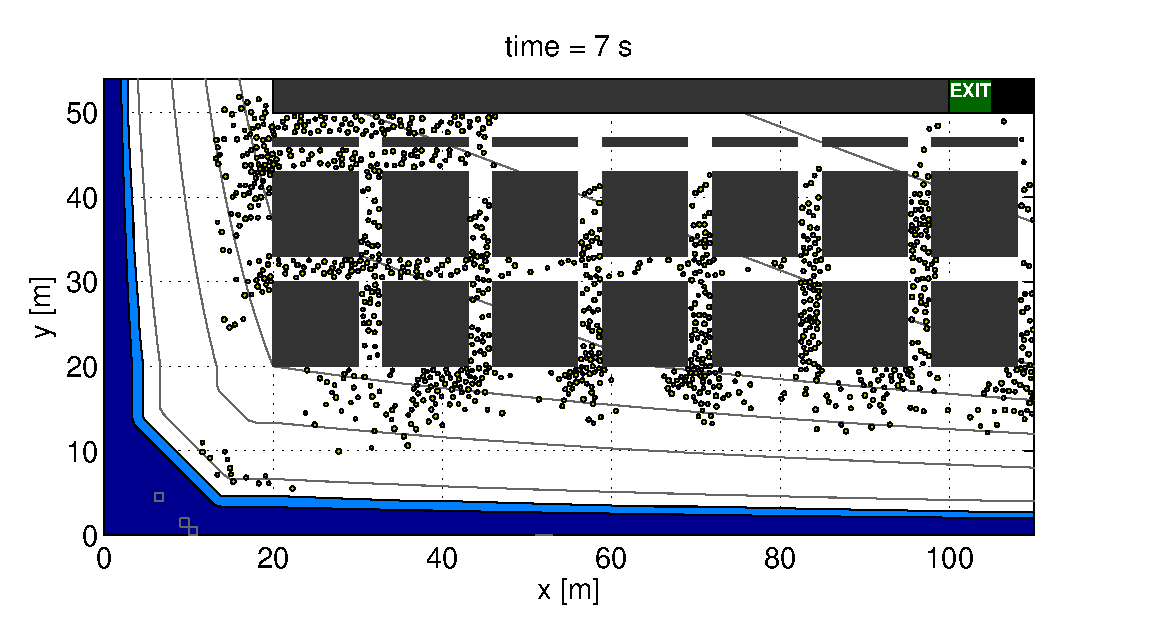
\includegraphics[width=1.1\textwidth]{figures/BeachEvacuationOneExitStreetWidth3_Flood0_1_000700.eps}
	\qquad
	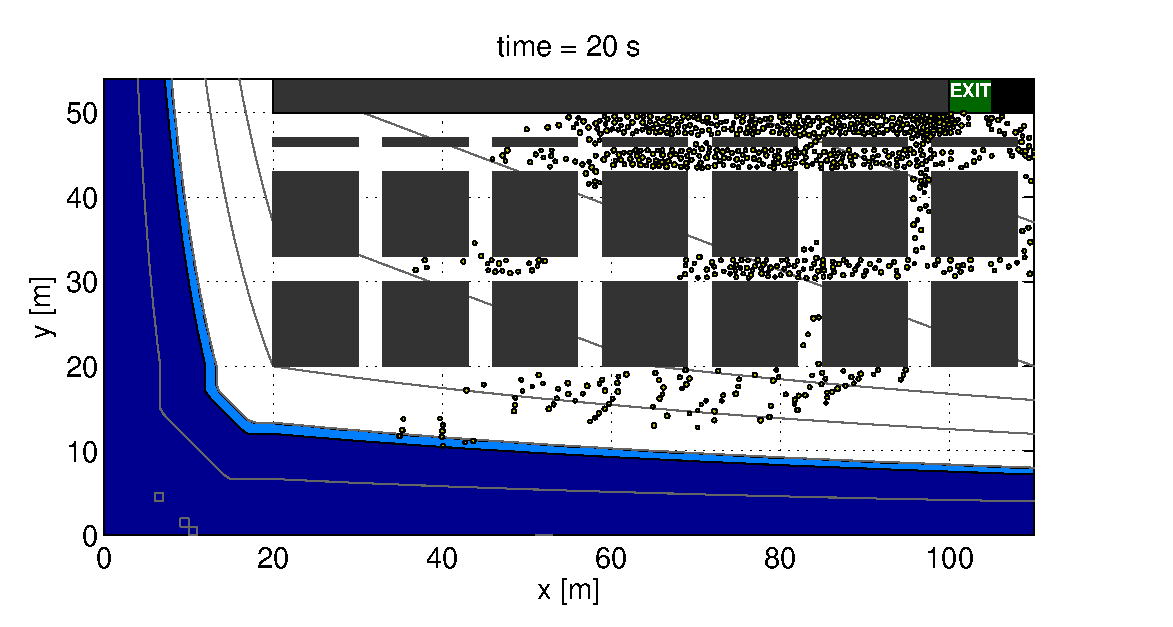
\includegraphics[width=1.1\textwidth]{figures/BeachEvacuationOneExitStreetWidth3_Flood0_1_002000.eps}
	\caption{Narrow beach house setup: different time steps show the approach of the flood and the escaping pedestrians.}
	\label{fig:beach_3}
\end{figure}

Fig.~\ref{fig:beach_3} presents an experiment with a narrow 3 m spacing between each house parcel. The pedestrians coming from the wide beach start to accumulate slightly at the house fronts in order to escape through the narrow paths. This slightly reduces the escape efficiency of this model.

\begin{figure}
	\centering
	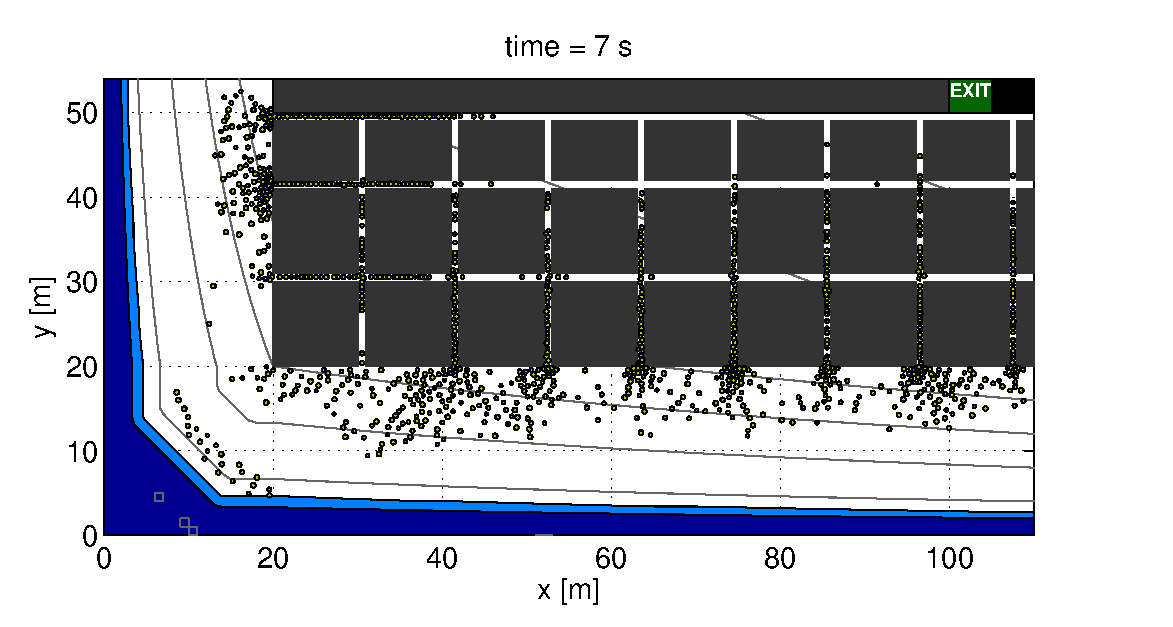
\includegraphics[width=1.1\textwidth]{figures/BeachEvacuationOneExitStreetWidth1_Flood0_1_000700.eps}
	\qquad
	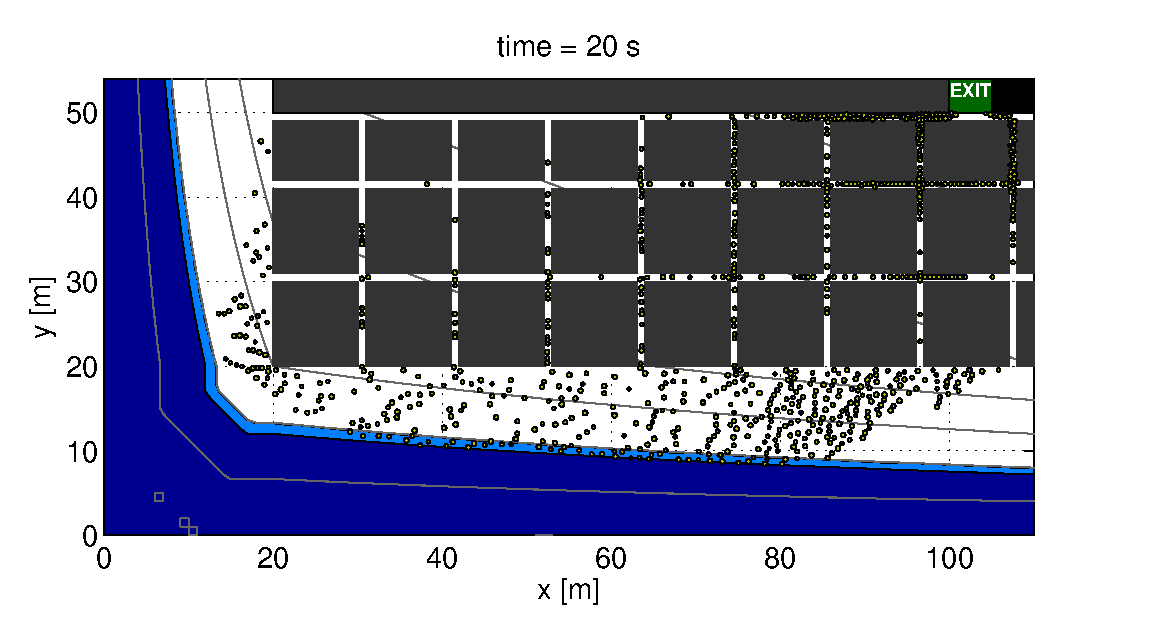
\includegraphics[width=1.1\textwidth]{figures/BeachEvacuationOneExitStreetWidth1_Flood0_1_002000.eps}
	\caption{Very narrow beach house setup: different time steps show the approach of the flood and the escaping pedestrians.}
	\label{fig:beach_4}
\end{figure}

Finally, the model setup with the narrowest house spacing (1 m between adjacent parcels) is shown in Fig.~\ref{fig:beach_4}. People now dramatically start to accumulate and the entering of the streets from the beach starts to become a bottleneck. Since the pedestrians are sensitive to the accumulation of a lot of people, they start to re-decide their exit path and try to find other ways out. This leads to a dense flow of people running on the beach parallel to the beach front until they eventually decide to head into a narrow street. This effectively hinders fast evacuation and hence, many people are caught by the rising water.

\begin{figure}
	\centering
	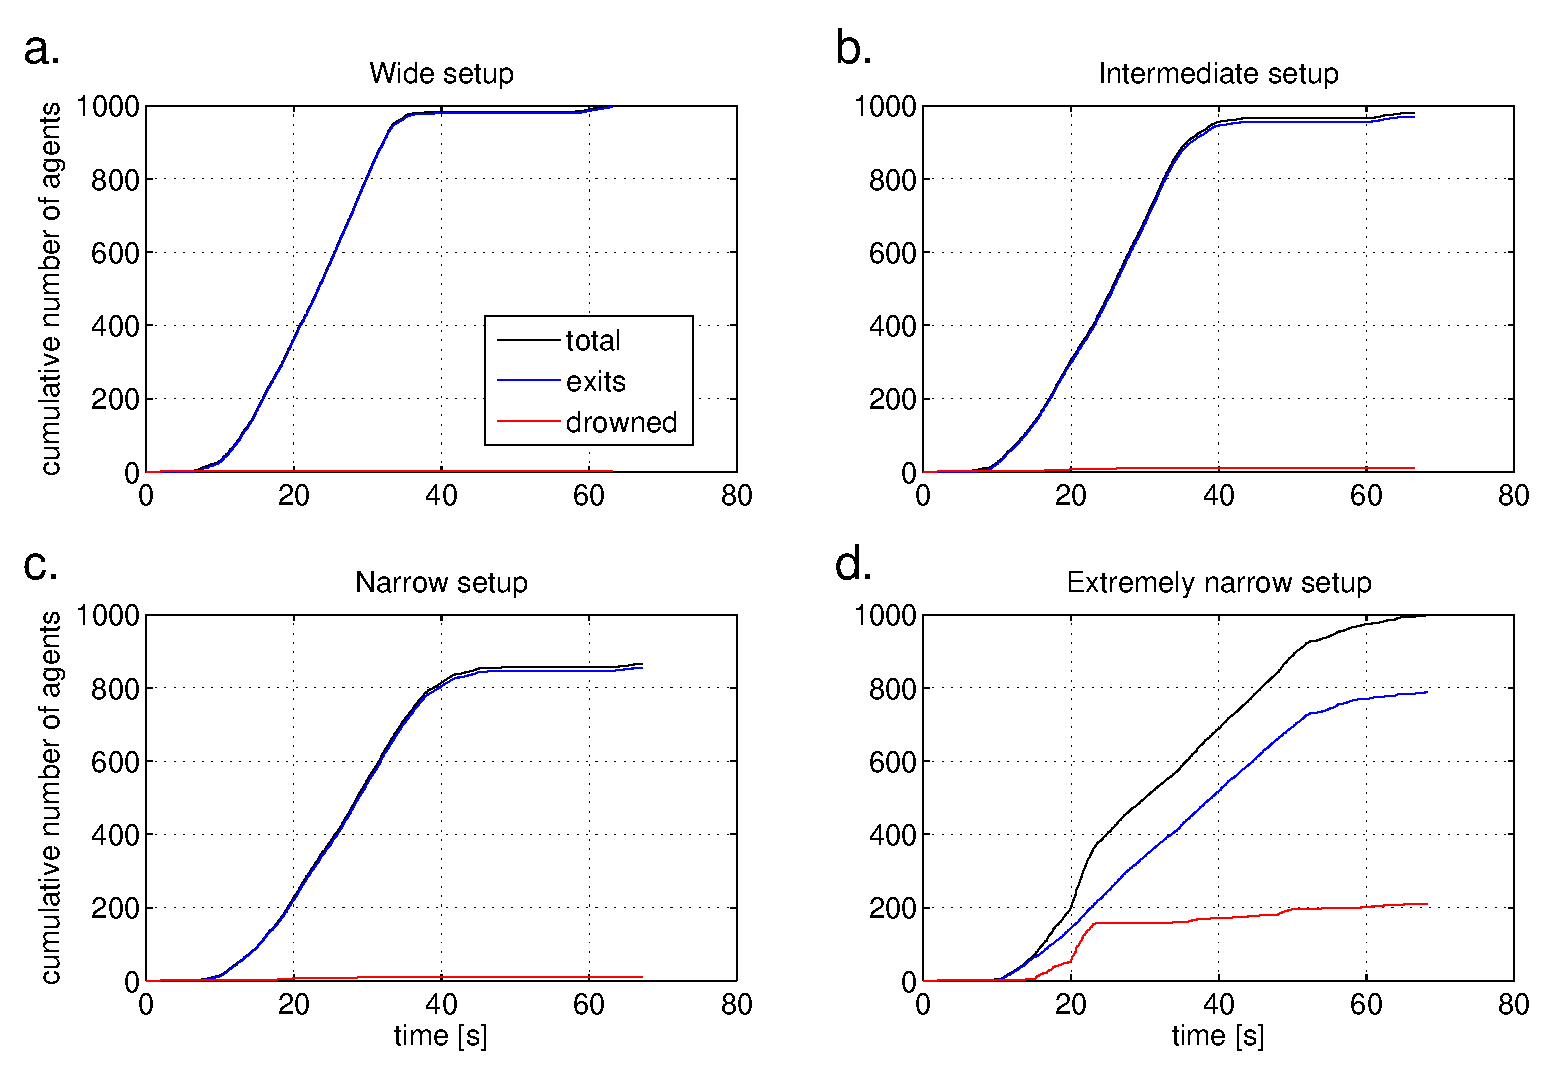
\includegraphics[width=1.1\textwidth]{figures/AnalysisMULTI_BeachEvacuationOneExitStreetWidth1_Flood0_1.eps}
	\caption{Escape efficiency for the different model setups. (a) Wide model setup with a street width of 7 m, (b) intermediate model setup with a street width of 5 m, (c) narrow model setup with a street width of 3 m and (d) extremely narrow model setup with a street width of 1 m. Curves show cumulative amount of people arrived at the exit (blue) or drowned in the flood (red) and the total of both (black).}
	\label{fig:analysis_1}
\end{figure}

To decide on the amount of buildings per beach area it is useful to look at the number of people that are able to exit the area in a sufficient short amount of time. This is done in Fig.~\ref{fig:analysis_1}, where the cumulative amount of people is plotted that are either able to exit the model domain or that are caught by the flood. Important is here the number of persons that are able to leave in a certain amount of time. The values are marked in Fig.~\ref{fig:analysis_1}, which shows decreasing values from 41 exits per time down to 18 exits per time by increasing the density of the house parcels. The amount of exits per time in the very dense model is so low, that a dramatical amount of people are drowned in the flood.

This leads us to the conclusion that the house parcel spacing needs to be larger than 1 m and can be as narrow as 3 m to guarantee economical prosperity that goes along with tourist savety.


\section{Summary and Outlook}

In this work we present an efficient numerical code that solves pedestrian flow and panic behaviour for large scale model setups as well as for a big number of agents. The model accuracy is benchmarked using a set of small model setups. Finally, the code is used give guidance in deciding about the beach house parcel spacing close to a beach. This is done by considering a possible flooding (i.e. rise of water level) and the subsequently upcoming escape panic. Parcel spacings of 3 m are shown to be sufficient, whereas a spacing of only 1 m leads to many dead people caused by the flood.

Still there are numerical issues which might be solved in future. The shortest path formulation that takes the position of the agents into account might be improved. It is not realistic, that one agent knows the positions of all the other pedestrians in the whole model domain, nor will he be able to decide physically correct on the shortest path in reality. On the other hand, numerical experiments like those presented in this study have to be taken into account in a decision process rather than considered as true nature. Thus, numerical models in social study might prevent many dramatic events in future and possibly already have done so.

\section{References}

\bibliographystyle{plainnat}
\bibliography{socialmodelling}


\begin{appendix}
\section{Code structure and source code}
In fig.\ref{fig:EscapePanic}., the basic structure of our code is shown. We split the code description in several different parts to provide a bit more readability. In principle, we tried to put most of the computations in separate functions. The input data and parameters necessary to run the simulation are all set in a separate input file, which then calls the actual simulation function. Rather than plotting the results "on the fly", the necessary data is saved regularly. Visualization is done in an postprocessing step.
\subsection{Input file}\label{sec:input_file}
In our input file, the user can set all the parameters that are needed. In tab.\ref{tab:input} and \ref{tab:input2}, we list all parameters that can be varied in the code, the  parameters we used and their effect.

\begin{table}
\begin{tabular}{l l l}
\hline
\textbf{Input parameter} & \textbf{value} & \textbf{meaning/effect}\\  
\hline
Parameter.Foldername & 'test' & name of the output folder\\
Parameter.Save & boolean & save output files or not\\
Parameter.SaveTimeStep & 10 & saves output every $n$ timesteps\\
Parameter.Resolution & 0.1 & resolution of the regular grid \\
Parameter.maxtime & 10 &maximum simulation time (in min)\\
Parameter.dt & 0.01 & simulation timestep\\
Parameter.nagent & 20-1000 & number of agents\\
Parameter.AgentSetup &random,given,load& determines the initial agent location\\
Parameter.m & 80 & agent mass in kg\\
Parameter.m\_pert & 10 & agent mass perturbation\\
Parameter.v & 5 & agent max velocity in m/s\\
Parameter.v\_pert & 5 & velocity perturbation\\
Parameter.t\_acc & 0.5 & acceleration time in s\\
Parameter.AgentSize & 0.25 & agent radius in m\\
Parameter.AgentSize\_pert & 0.05 & agent radius perturbation\\ 
Parameter.BoxSize\_pert & 5 & box size around agent\\ 
Parameter.PhysicalForces & boolean & switch physical forces on/off\\
Parameter.Tangential & boolean & switch tangential forces on/off\\
Parameter.k & 1.2e5 & phys. normal force prefactor\\
Parameter.kappa & 2.4e5 & phys. tangential force prefactor\\
Parameter.SocialForces & boolean & switch social forces on/off\\
Parameter.pert\_social & 0.05 & percentage of social force perturbation\\
Parameter.A & 2e3 & social force prefactor\\
Parameter.B & 0.08 & social force exponential factor\\
Parameter.ExitFactor & 1  & exit force prop. factor \\
Parameter.ExitForce & constant,proportional & constant or proportional exit force\\

\hline

\hline
\end{tabular}
\label{tab:input}
\caption{Input parameters for EscapePanic.m Part 1}
\end{table}


\begin{table}
\begin{tabular}{l l l}
\hline
\textbf{Input parameter} & \textbf{value} & \textbf{meaning/effect}\\  
\hline
Parameter.WithFlood & boolean & switch flooding on/ off\\
Parameter.z0\_flood & 0 & initial water height\\
Parameter.dzdt\_flood & 0.1 & rising rate\\
Parameter.dangerousDepth & 0.2 & if water depth is greater, agents drown\\
Parameter.FloodSpeed & $v_0/2$ & max velocity of agents in water\\
Parameter.A\_flood & 5e2 & social force parameter for flood\\
Parameter.B\_flood & 0.08 & social force parameter for flood\\ 
Parameter.DirectExitPath & boolean & use direct exit direction or not?\\
Parameter.orig\_sensitivity & 1 & sensitivity of agent to exit direction\\
& & without agents\\
Parameter.agent\_sensitivity & 2.5 & sens. of agents to others in the way\\
Parameter.topo\_sensitivity & 1 & not used anymore\\
Parameter.decision\_time & 0.05 & recompute shortest path after this time\\
Parameter.WithAgents & boolean & take agents into account?\\
Parameter.WithTopo & boolean & take topo into account?\\
Parameter.Enlarge & 0.3 & building enlargement \\
Parameter.Topo\_name & none,name & topo file to be used\\
Parameter.slope\_f & 3.5&factor for slope-dependent vel.\\
Parameter.slope\_crit & 0.05 & factor for slope-dependent vel.\\
Parameter.xmin & 0 & domain boundaries\\
Parameter.xmax & 20 - 50\\
Parameter.ymin & 0 \\
Parameter.ymax & 10-150\\

\hline

\hline
\end{tabular}
\label{tab:input2}
\caption{Input parameters for EscapePanic.m Part 2}
\end{table}
\begin{landscape}
\lstset{basicstyle=\footnotesize\ttfamily}
    
\begin{lstlisting}[breaklines]
%=================================
%
%       RUN ESCAPE PANIC
% 
%=================================
% Marcel Thielmann & Fabio Crameri

clear
%--------------------------------------------------------------------------
% run name
Parameter.Foldername        = 'test1';      % Run name
Parameter.Save              = logical(1);   % switch for saving output
Parameter.SaveTimeStep      = 200;          % saves every PlotTimeStep


%--------------------------------------------------------------------------
% numerical parameter
Parameter.resolution        = 0.1;          % resolution in [m]

Parameter.maxtime           = 3;            % maximum time to run in [min]
Parameter.dt                = 0.01;         % time step in [s]


%--------------------------------------------------------------------------
% number of agents
Parameter.nagent            = 50;           % number of agents

% agent parameters (can be perturbed with a random perturbation)
Parameter.AgentSetup        = 'random';     % 'random' 'given' 'load'
Parameter.m                 = 80;           % mass in kg
Parameter.m_pert            = 10;

Parameter.v0                = 1;            % maximal/desired velocity [m/s]
Parameter.v0_pert           = 0;   

Parameter.t_acc             = 0.5;        	% acceleration time in [s]

Parameter.AgentSize         = 0.25;         % agent radius
Parameter.AgentSize_pert    = 0.05; 

Parameter.BoxSize           = 5;            % agent box size


%--------------------------------------------------------------------------
% physical forces parameters (Helbing,2000)
Parameter.PhysicalForces    = true;
Parameter.Tangential        = false;
Parameter.k                 = 1.2e5;        %1.2e5 [Helbing 2000]
Parameter.kappa             = 2.4e5;        %2.4e5 [Helbing 2000]

% social force parameters
Parameter.SocialForces      = true;
Parameter.pert_social       = 0.0;          % maximal amplitude factor of social agent forces perturbation e.g. 0.05
Parameter.A                 = 2e3;          %[N]  [2e3 Helbing 2000]
Parameter.B                 = 0.08;         %[m]  [0.08 Helbing 2000]

Parameter.ExitForce         = 'constant';   %'constant' or 'proportional'
Parameter.ExitFactor        = 1;            %for adjusting strength of constant exit force field ...
                                            % absolute value if ExitForce='constant'


%--------------------------------------------------------------------------
% shortest path computation
Parameter.DirectExitPath    = false;     	% fast marching algorithm (false); direct exit line (true)

Parameter.orig_sensitivity	= 1;            % best to leave this fixed
Parameter.agent_sensitivity	= 2.5;            % how much are agents taken into account when computing the shortest path? [0: not taken into account - high value: taken into account]
Parameter.topo_sensitivity 	= 1;            % sensitivity of agents to topography

Parameter.decision_time   	= 0.05;         % after which time does an agent redecide on its path?

Parameter.WithAgents        = false;        % true or false, determines if agents are taken into account for shortest path computation
Parameter.WithTopo          = true;        % true or false, determines if topography is taken into account for shortest path computation

Parameter.Enlarge           = 0.2;          % enlarge buildings for shortest path formulation



%--------------------------------------------------------------------------
% flooding
Parameter.WithFlood         = true;        % true or false, determines if flood is taken into account for shortest path computation

Parameter.z0_flood          = 0;            % [m]
Parameter.dzdt_flood        = 0.01;         % rising speed of flood [m/s]
Parameter.dangerousDepth    = 0.2;          % [m]
Parameter.FloodSpeed        = Parameter.v0/2; % agents speed in shallow water [m/s]

Parameter.A_flood           = 5e2;          %[N]
Parameter.B_flood           = 0.08;         %[m]


%--------------------------------------------------------------------------
% topography
Parameter.Topo_name         = 'none';       % topography file to be loaded (if there is none, use 'none'), to set it off use 'off'

% parameters for slope-dependent velocity
Parameter.slope_f           = 3.5;
Parameter.slope_crit        = 0.05;


%--------------------------------------------------------------------------
% model domain
Parameter.xmin              = 0;
Parameter.xmax              = 20;
Parameter.ymin              = 0;
Parameter.ymax              = 10;

% create building list (if not given)
BuildingList                = [                 % coordinates of building xmin xmax ymin ymax
                                0 16 0 1        % boundary wall
                                0 16 9 10       % boundary wall
                                15 16 3 9       % top barriere
                                10 11 1 7       % bottom barriere
                                            ];
        
% create exit list (if not given)
ExitList                    = [                 % coordinates of exits: xmin xmax ymin ymax
                                19 20 4.5 5.5
                                            ];
       
% create starting area map for agents
StartingList                = [             	% coordinates of start area: xmin xmax ymin ymax
                                0.5 4 1.5 8.5
                                            ];
       
                                        
%--------------------------------------------------------------------------
%plotting parameters
Plotting.PlotEvolution      = true;             % direct plotting
Parameter.PlotTimeStep      = 50;               % plots every PlotTimeStep

Plotting.Marking            = 'none';           % 'none', 'number', 'smiley'
Plotting.FontSize           = 14;
Plotting.Color              = 'y';           % agents color: 'y' or [0 1 0]






%---------------------------------------
% test map
%---------------------------------------
% TestMap(Parameter,BuildingList,ExitList);      
       
%---------------------------------------
% run simulation
%---------------------------------------
EscapePanic(Parameter,BuildingList,ExitList,StartingList,Plotting);

\end{lstlisting}





\end{landscape}

\subsection{Beach evacution runs: Input file}\label{sec:input_file}
For the beach evacuation runs, we used two functions to create the building list and the topography. In the following, we list one example input file for the beach runs and the two additional functions.
\begin{landscape}
\lstset{basicstyle=\footnotesize\ttfamily}
    
\begin{lstlisting}[breaklines]
%=================================
%
%      This is BeachRun1.m
% 
%=================================
% Marcel Thielmann & Fabio Crameri

clear


%--------------------------------------------------------------------------
% run name
Parameter.Foldername        = 'BeachEvacuationOneExitStreetWidth5';      % Run name
Parameter.Save              = logical(1);   % switch for saving output
Parameter.SaveTimeStep      = 10;          % saves every PlotTimeStep

%--------------------------------------------------------------------------
% setup parameters
StreetWidth = 5;
BuildingWidthX = 10;
BuildingWidthY = 10;
BeachWidth = 20;
BeachHeight = 3;
MaxElevation = 7;

%--------------------------------------------------------------------------
% numerical parameter
Parameter.resolution        = 0.1;          % resolution in [m]

Parameter.maxtime           = 10;            % maximum time to run in [min]
Parameter.dt                = 0.01;         % time step in [s]


%--------------------------------------------------------------------------
% number of agents
Parameter.nagent            = 500;           % number of agents

% agent parameters (can be perturbed with a random perturbation)
Parameter.AgentSetup        = 'random';     % 'random' 'given' 'load'
Parameter.m                 = 80;           % mass in kg
Parameter.m_pert            = 10;

Parameter.v0                = 5;            % maximal/desired velocity [m/s]
Parameter.v0_pert           = 1;   

Parameter.t_acc             = 0.5;        	% acceleration time in [s]

Parameter.AgentSize         = 0.25;         % agent radius
Parameter.AgentSize_pert    = 0.05; 

Parameter.BoxSize           = 5;            % agent box size

%--------------------------------------------------------------------------
% physical forces parameters (Helbing,2000)
Parameter.PhysicalForces    = true;
Parameter.Tangential        = false;
Parameter.k                 = 1.2e5;        %1.2e5 [Helbing 2000]
Parameter.kappa             = 2.4e5;        %2.4e5 [Helbing 2000]

% social force parameters
Parameter.SocialForces      = true;
Parameter.pert_social       = 0.0;          % maximal amplitude factor of social agent forces perturbation e.g. 0.05
Parameter.A                 = 2e3;          %[N]  [2e3 Helbing 2000]
Parameter.B                 = 0.08;         %[m]  [0.08 Helbing 2000]
Parameter.ExitFactor        = 1;            %for adjusting strength of constant exit force field
Parameter.ExitForce = 'constant';

%--------------------------------------------------------------------------
% flooding
Parameter.WithFlood         = true;        % true or false, determines if flood is taken into account for shortest path computation

Parameter.z0_flood          = 0;            % [m]
Parameter.dzdt_flood        = 0.01;         % rising speed of flood [m/s]
Parameter.dangerousDepth    = 0.2;          % [m]
Parameter.FloodSpeed        = Parameter.v0/2; % agents speed in shallow water [m/s]

Parameter.A_flood           = 5e2;          %[N]
Parameter.B_flood           = 0.08;         %[m]

%--------------------------------------------------------------------------
% shortest path computation
Parameter.DirectExitPath    = false;     	% fast marching algorithm (false); direct exit line (true)

Parameter.orig_sensitivity	= 1;            % best to leave this fixed
Parameter.agent_sensitivity	= 2.5;            % how much are agents taken into account when computing the shortest path? [0: not taken into account - high value: taken into account]
Parameter.topo_sensitivity 	= 1;            % sensitivity of agents to topography

Parameter.decision_time   	= 0.05;         % after which time does an agent redecide on its path?

Parameter.WithAgents        = true;        % true or false, determines if agents are taken into account for shortest path computation
Parameter.WithTopo          = false;        % true or false, determines if topography is taken into account for shortest path computation

Parameter.Enlarge           = 0.3;          % enlarge buildings for shortest path formulation


%--------------------------------------------------------------------------
% topography
Parameter.Topo_name         = 'BeachTopo';       % topography file to be loaded (if there is none, use 'none')

% parameters for slope-dependent velocity
Parameter.slope_f           = 3.5;
Parameter.slope_crit        = 0.05;


%--------------------------------------------------------------------------
% model domain
Parameter.xmin              = 0;
Parameter.xmax              = 150;
Parameter.ymin              = 0;
Parameter.ymax              = 54;

% create building list (if not given)


% create buildings on beach
x_min_build = Parameter.xmin + BeachWidth;
x_max_build = Parameter.xmax;
y_min_build = Parameter.ymin + BeachWidth;
y_max_build = Parameter.ymax-StreetWidth-4; % leave 4 meters for "dam"
DomainWidth = x_max_build-x_min_build;
DomainHeight = y_max_build-y_min_build;
BuildingList = SetBuildings(DomainWidth,DomainHeight,StreetWidth,BuildingWidthX,BuildingWidthY); % for beach houses

% shift building list values by real min values
BuildingList(:,1:2) = BuildingList(:,1:2) + x_min_build;
BuildingList(:,3:4) = BuildingList(:,3:4) + y_min_build;

BuildingList                = [ BuildingList                % coordinates of building xmin xmax ymin ymax
                                BeachWidth 100 Parameter.ymax-4 Parameter.ymax        % boundary wall
                                105 180 Parameter.ymax-4 Parameter.ymax       % boundary wall
                                185 200 Parameter.ymax-4 Parameter.ymax
                                
                                            ];
        
% create exit list (if not given)
ExitList                    = [                 % coordinates of exits: xmin xmax ymin ymax
                                100 105 Parameter.ymax-4 Parameter.ymax
                                180 185 Parameter.ymax-4 Parameter.ymax
                                            ];
       
% create starting area map for agents
StartingList                = [             	% coordinates of start area: xmin xmax ymin ymax
                                0 BeachWidth Parameter.ymin Parameter.ymax
                                0 Parameter.xmax Parameter.ymin BeachWidth
                                            ];
       
                                        
%--------------------------------------------------------------------------
%plotting parameters
Plotting.PlotEvolution      = false;             % direct plotting
Parameter.PlotTimeStep      = 100;               % plots every PlotTimeStep

Plotting.Marking            = 'none';           % 'none', 'number', 'smiley'
Plotting.FontSize           = 14;
Plotting.Color              = 'y';           % agents color: 'y' or [0 1 0]


%---------------------------------------
% test map
%---------------------------------------
% TestMap(Parameter,BuildingList,ExitList);
if ~strcmp(Parameter.Topo_name,'none')
    CreateTopo;
    save(Parameter.Topo_name,'XTopo','YTopo','ZTopo');
end
%---------------------------------------
% run simulation
%---------------------------------------
EscapePanic(Parameter,BuildingList,ExitList,StartingList,Plotting);

\end{lstlisting}





\lstset{basicstyle=\footnotesize\ttfamily}
    
\begin{lstlisting}[breaklines]
%=======================================
% This is CreateTopo.m
%=======================================


% function [XTopo,YTopo,ZTopo] = CreateTopo(Parameter,BeachWidth,BeachHeight,MaxElevation)

% Create topography

[XTopo,YTopo] = meshgrid(Parameter.xmin:Parameter.xmax,Parameter.ymin:Parameter.ymax);

% create building topo
DomainWidth = (Parameter.xmax-Parameter.xmin)-BeachWidth;
DomainHeight = (Parameter.ymax-Parameter.ymin)-BeachWidth;

mx = (MaxElevation-BeachHeight)/DomainWidth;
my = (MaxElevation-BeachHeight)/DomainHeight;

[x_bt,y_bt] = meshgrid(0:DomainWidth,0:DomainHeight);

z_bt = mx*x_bt + my*y_bt + BeachHeight;

x_bt = x_bt + BeachWidth;
y_bt = y_bt + BeachWidth;


x1 = Parameter.xmin:Parameter.xmax;
y1 = 0*x1;
z1 = 0*x1;

y2 = Parameter.ymin:Parameter.ymax;
x2 = 0*y2;
z2 = 0*y2;

x = [x_bt(:);x1';x2'];
y = [y_bt(:);y1';y2'];
z = [z_bt(:);z1';z2'];

z = max(-0.4,z);

ZTopo = 0*XTopo;
ZTopo(:) = griddata(x,y,z,XTopo,YTopo);
    
\end{lstlisting}

\lstset{basicstyle=\footnotesize\ttfamily}
    
\begin{lstlisting}[breaklines]
%=================================================
% This is SetBuildings.m
%=================================================


% function to generate the building list for the beach setup
function BuildingList = SetBuildings(DomainWidth,DomainHeight,StreetWidth,BuildingWidthX,BuildingWidthY)



% x-direction
i = 1;
x_min_vec(i) = 0;
x_max_vec(i) = x_min_vec(i)+BuildingWidthX;

while x_min_vec(i)<DomainWidth
    i=i+1;
    x_min_vec(i) = x_min_vec(i-1)+BuildingWidthX+StreetWidth;
    x_max_vec(i) = x_max_vec(i-1)+BuildingWidthX+StreetWidth;
    
    
    
    if x_max_vec(i) > DomainWidth
        x_max_vec(i) = DomainWidth;
    end
end

if x_min_vec(end) >= x_max_vec(end)
    x_min_vec(end) = [];
    x_max_vec(end) = [];
end
% y-direction

i = 1;
y_min_vec(i) = 0;
y_max_vec(i) = y_min_vec(i)+BuildingWidthY;

while y_min_vec(i)<DomainHeight
    i=i+1;
    y_min_vec(i) = y_min_vec(i-1)+BuildingWidthY+StreetWidth;
    y_max_vec(i) = y_max_vec(i-1)+BuildingWidthY+StreetWidth;
    if y_max_vec(i) > DomainHeight
        y_max_vec(i) = DomainHeight;
    end
end
if y_min_vec(end) >= y_max_vec(end) 
    y_min_vec(end) = [];
    y_max_vec(end) = [];
end


[XMIN,YMIN] = meshgrid(x_min_vec,y_min_vec);
[XMAX,YMAX] = meshgrid(x_max_vec,y_max_vec);


BuildingList = [XMIN(:) XMAX(:) YMIN(:) YMAX(:)];

\end{lstlisting}
\end{landscape}
\subsection{Simulation function}
The simulation function that is called by the input file runs the entire simulation, saves the output and plots intermediate results if desired. Before entering the time loop, a number of actions is performed (see fig.\ref{fig:pre-loop}). The computation of all forces that do not change throughout the simulation is done here. After the pre-loop stage, we enter the time loop. In here, we perform a number of computations for all agents, before entering an agent loop, in which we compute individual and agent-specific parameters (see fig.\ref{fig:EscapePanic}). After completing the time loop, some parameters for later analysis are save and the function exits. 

Source code files are listed in the order of their appearance.
\begin{landscape}

\lstset{basicstyle=\footnotesize\ttfamily}
    
    \begin{lstlisting}[breaklines]
%=================================
%          ESCAPE PANIC
%       including flooding
%=================================
% Marcel Thielmann & Fabio Crameri

function [AGENT] = EscapePanic(Parameter,BuildingList,ExitList,StartingList,Plotting)

% if nargin == 0
%     clear;
%     **************************************************
%     Marcels:
%     TwoExitsStandardSetup;
%     **************************************************
%     Fabios:
%     [Parameter,BuildingList,ExitList,StartingList,Plotting] = SetupModel;
%     **************************************************
% end


% workflow control
PlotSetup       = false;
PlotEvolution   = Plotting.PlotEvolution;

DirectExitPath  = Parameter.DirectExitPath;
WithAgents      = Parameter.WithAgents;
WithTopo        = Parameter.WithTopo;
WithFlood       = Parameter.WithFlood;
Z_flood         = Parameter.z0_flood;    dzdt_flood = Parameter.dzdt_flood;
dangerousDepth  = Parameter.dangerousDepth;

%==========================================================================
% add necessary paths
%==========================================================================
addpath ../DecisionStrategy/
addpath ../WallForces/
addpath ../Plotting/
addpath ../kdtree_alg_OSX/
addpath ../FastMarching_version3b, add_function_paths();

%==========================================================================
% initialize grid
%==========================================================================
resolution          = Parameter.resolution;
xmin                = Parameter.xmin;
xmax                = Parameter.xmax;
ymin                = Parameter.ymin;
ymax                = Parameter.ymax;

xvec                = xmin:resolution:xmax;
yvec                = ymin:resolution:ymax;
[X_Grid,Y_Grid]     = meshgrid(xvec,yvec);

% set topography
if (strcmp(Parameter.Topo_name,'none') && WithTopo)
    A = 2;
    x0 = 10;
    y0 = 5;
    sigma_x = 15;
    sigma_y = 6;
    Z_Grid = A.*exp(-1*( (X_Grid-x0).^2/2/sigma_x     + (Y_Grid-y0).^2/2/sigma_y ));
elseif (strcmp(Parameter.Topo_name,'none') && ~WithTopo) || strcmp(Parameter.Topo_name,'off')
    Z_Grid = 0.*X_Grid;
else
    load(Parameter.Topo_name);
    Z_Grid = interp2(XTopo,YTopo,ZTopo,X_Grid,Y_Grid);
end

% saves setup
if Parameter.Save
    filestem = ['../+output/',Parameter.Foldername];
    if ~exist(filestem,'dir'); mkdir(filestem); end

    save(['../+output/',Parameter.Foldername,'/Setup.mat'])
end

% compute topography gradient
[Gradient_x,Gradient_y] = gradient(Z_Grid,resolution,resolution);

%convert time
maxtime         = Parameter.maxtime*60; %[min] => [s]
decision_step   = round(Parameter.decision_time/Parameter.dt);

%---------------------------------------
% create starting area map for agents
%---------------------------------------
StartingList(find(StartingList(:,1)>=xmax),:) = []; %if set fully outside domain: remove it!
StartingList(find(StartingList(:,3)>=ymax),:) = []; %if set fully outside domain: remove it!
StartingList(find(StartingList(:,2)>xmax),2) = xmax; %adjust to domain boundary
StartingList(find(StartingList(:,4)>ymax),2) = ymax; %adjust to domain boundary

StartArea = logical(X_Grid*0);
% add buildings to map
for i=1:size(StartingList,1)
    StartArea(X_Grid>=StartingList(i,1) & X_Grid<=StartingList(i,2) & Y_Grid>=StartingList(i,3) & Y_Grid<=StartingList(i,4)) = true;
end

%---------------------------------------
% create boundary map for later use
%---------------------------------------
BoundaryMap = zeros(size(yvec,2),size(xvec,2));
BoundaryMap(1,:)=1; BoundaryMap(size(yvec,2),:)=1; BoundaryMap(:,1)=1; BoundaryMap(:,size(xvec,2))=1;

%---------------------------------------
% create building map for later use
%---------------------------------------
BuildingList(find(BuildingList(:,1)>=xmax),:) = []; %if building fully outside domain: remove it!
BuildingList(find(BuildingList(:,3)>=ymax),:) = []; %if building fully outside domain: remove it!
BuildingList(find(BuildingList(:,2)>xmax),2) = xmax; %adjust building to domain boundary
BuildingList(find(BuildingList(:,4)>ymax),2) = ymax; %adjust building to domain boundary

BuildingMap = logical(X_Grid*0);  BuildingMap_sp = BuildingMap;
% add buildings to map
for i=1:size(BuildingList,1)
    BuildingMap(X_Grid>=BuildingList(i,1) & X_Grid<=BuildingList(i,2) & Y_Grid>=BuildingList(i,3) & Y_Grid<=BuildingList(i,4)) = true;
    %for shortest path formulation:
    BuildingMap_sp(X_Grid>=(BuildingList(i,1)-Parameter.Enlarge) & X_Grid<=(BuildingList(i,2)+Parameter.Enlarge) ...
        & Y_Grid>=(BuildingList(i,3)-Parameter.Enlarge) & Y_Grid<=(BuildingList(i,4)+Parameter.Enlarge) ) = true;
end

%-----------------------------------------------------------------
% create exit map for later use and compute center point of exits
%-----------------------------------------------------------------
ExitList(find(ExitList(:,1)>=xmax),:)   = []; %if exit fully outside domain: remove it!
ExitList(find(ExitList(:,3)>=ymax),:)   = []; %if exit fully outside domain: remove it!
ExitList(find(ExitList(:,2)>xmax),2)    = xmax; %adjust exit to domain boundary
ExitList(find(ExitList(:,4)>ymax),2)    = ymax; %adjust exit to domain boundary

ExitMap = logical(X_Grid*0);
for i=1:size(ExitList,1)
    ExitMap(X_Grid>=ExitList(i,1) & X_Grid<=ExitList(i,2) & Y_Grid>=ExitList(i,3) & Y_Grid<=ExitList(i,4)) = true;
end

%----------------------------------------------------
% create flood map
%----------------------------------------------------
%compute height
Z_flood_deep = Z_flood - dangerousDepth;

%create floodmap
FloodMap = logical(X_Grid*0); FloodMap_deep = FloodMap;
FloodHeightMap = ones(size(Z_Grid))*Z_flood;
FloodMap(FloodHeightMap>Z_Grid) = 1;
FloodHeightMap_deep = ones(size(Z_Grid))*Z_flood_deep;
FloodMap_deep(FloodHeightMap_deep>Z_Grid) = 1;

% initialize agents
nagent  = Parameter.nagent;
AGENT   = InitializeAgents(nagent,Parameter);

% create random agent distribution
if strcmp(Parameter.AgentSetup,'random')
    AGENT   = CreateInitialAgentDistribution(nagent,AGENT,X_Grid,Y_Grid,BuildingMap,BoundaryMap,StartArea,ExitMap);
elseif strcmp(Parameter.AgentSetup,'given')
    cell_array = num2cell(AgentX);
    [AGENT(1:nagent).LocX]      = cell_array{:};
    cell_array = num2cell(AgentY);
    [AGENT(1:nagent).LocY]      = cell_array{:};
elseif strcmp(Parameter.AgentSetup,'load')
    load(Parameter.AgentLocationFile);
    cell_array = num2cell(AgentX);
    [AGENT(1:nagent).LocX]      = cell_array{:};
    cell_array = num2cell(AgentY);
    [AGENT(1:nagent).LocY]      = cell_array{:};
end

%----------------------------------------------------
% building locations
%----------------------------------------------------
x_Buildings = X_Grid(BuildingMap);
y_Buildings = Y_Grid(BuildingMap);

%----------------------------------------------------
% compute forces from buildings (static)
%----------------------------------------------------
[ArchForce,ArchD,ArchDirX,ArchDirY] = ArchitectureForceV2(X_Grid,Y_Grid,BuildingMap,Parameter,resolution);




%----------------------------------------------------
% compute shortest path to exit
%----------------------------------------------------
BuildingMap_boundary = zeros(size(BuildingMap)); BuildingMap_boundary(BuildingMap~=BuildingMap_sp) = 1;
if (~DirectExitPath && ~WithTopo)
    % compute shortest path without topography with fast marchng algorithm
    [Dgradx,Dgrady,D_orig] = ComputeShortestPathGlobal(FloodMap,FloodMap_deep,BuildingMap,BuildingMap_boundary,ExitMap,X_Grid,Y_Grid,Parameter);
elseif (~DirectExitPath && WithTopo)
    % compute shortest path without topography with fast marchng algorithm
    [~,~,D_orig] = ComputeShortestPathGlobal(FloodMap,FloodMap_deep,BuildingMap,BuildingMap_boundary,ExitMap,X_Grid,Y_Grid,Parameter);
    % compute shortest path with topography with fast marchng algorithm
    [Dgradx,Dgrady,D_orig] = ComputeShortestPathGlobalTopo(FloodMap,FloodMap_deep,BuildingMap,BuildingMap_boundary,ExitMap,X_Grid,Y_Grid,Z_Grid,D_orig,Gradient_x,Gradient_y,Parameter);
elseif DirectExitPath
    % compute exit direction directly
    [Dgradx,Dgrady] = ComputeShortestPathGlobalDirect(BuildingMap,ExitMap,X_Grid,Y_Grid,Parameter.v0,Parameter.resolution);
end

%----------------------------------------------------
% plot setup
%----------------------------------------------------
if PlotSetup
    % plot setup
    figure(1),clf
    set(cla,'FontSize',Plotting.FontSize)
    hold on
    % plot buildings
    PlotBuildings(BuildingList,'r','');
    PlotBuildings(ExitList,'g','Exit');
    % plot agents
    PlotAgents(AGENT,Plotting);
    axis equal
    axis([min(X_Grid(:)) max(X_Grid(:)) min(Y_Grid(:)) max(Y_Grid(:))])
    box on
    title('time = 0.00 min')
    xlabel('x [m]')
    ylabel('y [m]')
end

%----------------------------------------------------
% save data (INITIAL SETUP)
%----------------------------------------------------
if Parameter.Save
    filestem = ['../+output/',Parameter.Foldername];
    if ~exist(filestem,'dir'); mkdir(filestem); end
    filename_full = [filestem,'/',Parameter.Foldername,'_',num2str(0,'%5.6d')];
    save(filename_full,'AGENT')
end

%setup analysis variable
%Analysis = [num/name startPosX startPosY ExitTime Status]
%                                       Status:	:   1:  'alive' still running
%                                                   2:  'survived' reached exit
%                                                   3:  'killed' e.g. by flood
Analysis        = zeros(nagent,5)*NaN;
Analysis(:,1)   = [AGENT.name]';
Analysis(:,2)   = [AGENT.LocX]';
Analysis(:,3)   = [AGENT.LocY]';
Analysis(:,5)   = 1;



%==========================================================================
% time loop
time=0; itime=0;
while (time <= maxtime && size(AGENT,2)>0)
    time = time+Parameter.dt;     %actual time [s]
    itime = itime+1;    %nr. timesteps
    disp('*****************************************')
    disp(['timestep ',num2str(itime),':    time = ',num2str(time/60),' min'])

    if sum(isnan([AGENT.LocX]))
        error('NaN');
    end

    %----------------------------------------------------
    % interpolate z-level Agent
    %----------------------------------------------------
    agent_Locz = interp2(X_Grid,Y_Grid,Z_Grid,[AGENT.LocX],[AGENT.LocY],'*linear');
    dummy                     	= num2cell(agent_Locz);
    [AGENT(1:nagent).LocZ]  	= dummy{:};

    %----------------------------------------------------
    % compute flooding
    %----------------------------------------------------
    if WithFlood
        %compute height
        Z_flood  = Z_flood + dzdt_flood*Parameter.dt;
        Z_flood_deep = Z_flood - dangerousDepth;

        %create floodmap
        FloodMap = logical(X_Grid*0); FloodMap_deep = FloodMap;
        FloodHeightMap = ones(size(Z_Grid))*Z_flood;
        FloodMap(FloodHeightMap>Z_Grid) = 1;
        FloodHeightMap_deep = ones(size(Z_Grid))*Z_flood_deep;
        FloodMap_deep(FloodHeightMap_deep>Z_Grid) = 1;

        % compute forces from flood
        if (Z_flood>min(min(Z_Grid))) % for shallow part
            [FloodForce,~,FloodDirX,FloodDirY] = f_FloodForce(X_Grid,Y_Grid,FloodMap,Parameter,resolution);
            % compute forces from flood (2nd part) on all agents
            % and interpolate it to the agent
            [FxSocialFlood,FySocialFlood] = ComputeSocialForcesStatic_flood(AGENT,X_Grid,Y_Grid,FloodForce,FloodDirX,FloodDirY,Parameter);
            dummy                                 = num2cell(FxSocialFlood);
            [AGENT(1:nagent).FxSocialFlood]       = dummy{:};
            dummy                                 = num2cell(FySocialFlood);
            [AGENT(1:nagent).FySocialFlood]       = dummy{:};
        end
        if (Z_flood_deep>min(min(Z_Grid))) % for deep part
            [FloodForce_deep,~,FloodDirX_deep,FloodDirY_deep] = f_FloodForce(X_Grid,Y_Grid,FloodMap_deep,Parameter,resolution);
            % compute forces from flood (2nd part) on all agents
            % and interpolate it to the agent
            [FxSocialFlood_deep,FySocialFlood_deep] = ComputeSocialForcesStatic_flood(AGENT,X_Grid,Y_Grid,FloodForce_deep,FloodDirX_deep,FloodDirY_deep,Parameter);
            dummy                             	= num2cell([AGENT(1:nagent).FxSocialFlood] + FxSocialFlood_deep);
            [AGENT(1:nagent).FxSocialFlood]     = dummy{:}; %add to shallow flood force
            dummy                              	= num2cell([AGENT(1:nagent).FySocialFlood] + FySocialFlood_deep);
            [AGENT(1:nagent).FySocialFlood]     = dummy{:}; %add to shallow flood force
        end
    end

    %----------------------------------------------------
    % compute kdtree of agents for later use
    %----------------------------------------------------
    ReferencePoints         = zeros(nagent,2);
    ReferencePoints(:,1)    = [AGENT(:).LocX];
    ReferencePoints(:,2)    = [AGENT(:).LocY];

    % generate tree
    tree =   kdtree(ReferencePoints);

    %----------------------------------------------------
    % compute forces from buildings (2nd part) on all agents
    % and interpolate it to the agent
    %----------------------------------------------------
    if Parameter.SocialForces
        [FxSocialWalls,FySocialWalls] = ComputeSocialForcesStatic(AGENT,X_Grid,Y_Grid,ArchForce,ArchDirX,ArchDirY,Parameter);
        dummy                                 = num2cell(FxSocialWalls);
        [AGENT(1:nagent).FxSocialWalls]       = dummy{:};
        dummy                                 = num2cell(FySocialWalls);
        [AGENT(1:nagent).FySocialWalls]       = dummy{:};
    else
        [AGENT(1:nagent).FxSocialWalls]       = deal(0);
        [AGENT(1:nagent).FySocialWalls]       = deal(0);
    end

    %----------------------------------------------------
    % compute direction field to exits on all agents
    % (just interpolate the precomputed field to the agents)
    %----------------------------------------------------
    if (~DirectExitPath && WithAgents)
        if (mod(itime,decision_step)==0 || itime==1)
            [Dgradx,Dgrady] = ComputeShortestPathGlobalWithAgents(BuildingMap,BuildingMap_boundary,...
                ExitMap,X_Grid,Y_Grid,D_orig,Dgradx,Dgrady,Gradient_x,Gradient_y,AGENT,nagent,Parameter);
        end
    elseif (~DirectExitPath && WithAgents && WithFlood)
        if (mod(itime,decision_step)==0 || itime==1)
            [Dgradx,Dgrady] = ComputeShortestPathGlobalWithAgentsFlood(FloodMap,FloodMap_deep,BuildingMap,BuildingMap_boundary,...
                ExitMap,X_Grid,Y_Grid,D_orig,Dgradx,Dgrady,Gradient_x,Gradient_y,AGENT,nagent,Parameter);
        end
    end

    xExitDirAgents = interp2(X_Grid,Y_Grid,Dgradx,[AGENT.LocX],[AGENT.LocY],'*linear');
    yExitDirAgents = interp2(X_Grid,Y_Grid,Dgrady,[AGENT.LocX],[AGENT.LocY],'*linear');

%     % normalize direction vector
%     dirtot         = sqrt(xExitDirAgents.^2+yExitDirAgents.^2);
%     xExitDirAgents = xExitDirAgents./dirtot;
%     yExitDirAgents = yExitDirAgents./dirtot;

    dummy = num2cell(xExitDirAgents);
    [AGENT(1:nagent).xExitDir]       = dummy{:};
    dummy = num2cell(yExitDirAgents);
    [AGENT(1:nagent).yExitDir]       = dummy{:};


    %----------------------------------------------------
    % agent loop
    iagent=0; nagent2 = nagent;
    for iagent = 1:nagent2
        x_agent         = AGENT(iagent).LocX;
        y_agent         = AGENT(iagent).LocY;
        agent_size      = AGENT(iagent).Size;
        velx_agent      = AGENT(iagent).VelX;
        vely_agent      = AGENT(iagent).VelY;

        %-------------------------------------------------
        % check if the agent is outside the domain
        %-------------------------------------------------
        if x_agent>xmax || x_agent<xmin || y_agent>ymax || y_agent<ymin
           error('fc: stupid agent outside domain!')
        end

        %-------------------------------------------------
        % get the agents that are in the "individual box" and compute the
        % distance to them
        %-------------------------------------------------
        [AGENT,x_others,y_others,others_size] = GetSurroundingAgents(iagent,AGENT,tree);

        [Normal,Tangent,DistanceToAgents,num_others] = ComputeDistanceToAgents(x_agent,y_agent,agent_size,x_others,y_others,others_size);

        if num_others >0
            % find agents that are too close
            indTooClose     = find(DistanceToAgents>=0);

            %----------------------------------------------------
            % compute social forces from other agents and apply a weighting
            % function to simulate that agents only have a reduced field of
            % vision
            %----------------------------------------------------
            if Parameter.SocialForces
                [FxAgentsSocial,FyAgentsSocial] = ComputeSocialForcesDynamic(Parameter,DistanceToAgents,Normal);
            else
                FxAgentsSocial = 0;
                FyAgentsSocial = 0;
            end

            %----------------------------------------------------
            % compute physical forces from other agents
            %----------------------------------------------------
            if (~isempty(indTooClose) && Parameter.PhysicalForces)
                surr_agents     = AGENT(iagent).SurroundingAgents;
                AgentTooClose   = surr_agents(indTooClose);
                DistTooClose    = DistanceToAgents(indTooClose);

                velx_others = AGENT(AgentTooClose).VelX;
                vely_others = AGENT(AgentTooClose).VelY;

                [FxPhysAgents,FyPhysAgents] = ComputePhysicalForceAgents(velx_agent,vely_agent,velx_others,vely_others,Parameter,DistTooClose,Normal(indTooClose,:),Tangent(indTooClose,:));
            else
                FxPhysAgents = 0;
                FyPhysAgents = 0;
            end
        else
            FxAgentsSocial = 0;
            FyAgentsSocial = 0;
            FxPhysAgents = 0;
            FyPhysAgents = 0;
        end

        %----------------------------------------------------
        % compute physical forces from walls
        %----------------------------------------------------
        if Parameter.PhysicalForces
            [FxPhysWall,FyPhysWall] = ComputePhysicalForceWalls(x_agent,y_agent,agent_size,velx_agent,vely_agent,x_Buildings,y_Buildings,Parameter);
        else
            FxPhysWall = 0;
            FyPhysWall = 0;
        end

        %----------------------------------------------------
        % assign forces to structure
        %----------------------------------------------------
        AGENT(iagent).FxPhysAgents   = sum(FxPhysAgents);
        AGENT(iagent).FyPhysAgents   = sum(FyPhysAgents);
        AGENT(iagent).FxPhysWall     = sum(FxPhysWall);
        AGENT(iagent).FyPhysWall     = sum(FyPhysWall);

        % add some random noise on the social force from other agents
        AGENT(iagent).FxSocialAgents = sum(FxAgentsSocial)*(1+ Parameter.pert_social*(-0.5+rand(1)) );
        AGENT(iagent).FySocialAgents = sum(FyAgentsSocial)*(1+ Parameter.pert_social*(-0.5+rand(1)) );
    end

    %----------------------------------------------------
    % compute exit force
    %----------------------------------------------------
    [AGENT] = ComputeExitForce(AGENT,Parameter,nagent);

    %----------------------------------------------------
    % check if agents in flood
    %----------------------------------------------------
    wet = [AGENT( [AGENT.LocZ]<=Z_flood ).num];
    if ~isempty(wet)
        for iwet=1:size(wet,2)
            AGENT(wet(1,iwet)).Status = 2; %wet
            AGENT(wet(1,iwet)).VMax = Parameter.FloodSpeed; %decrease max. speed by half VMax
        end
    end

    %----------------------------------------------------
    % move agents
    %----------------------------------------------------
    [AGENT] = MoveAgents(AGENT,X_Grid,Y_Grid,Gradient_x,Gradient_y,Parameter.dt,nagent,Parameter);

    %----------------------------------------------------
    % check if agents are inside walls and move them out
    %----------------------------------------------------
    AGENT = CheckAgentsInBuildings(AGENT,BuildingList,X_Grid,Y_Grid,ArchDirX,ArchDirY,ArchD);

    %----------------------------------------------------
    % remove successfull/dead agents
    %----------------------------------------------------
    %those who arrived in the exits
    for i=1:size(ExitList,1)
        successfull = [AGENT(  [AGENT.LocX]>=ExitList(i,1) & [AGENT.LocX]<=ExitList(i,2) ...
            & [AGENT.LocY]>=ExitList(i,3) & [AGENT.LocY]<=ExitList(i,4) ).num];
        %save time of agents exit
        Analysis([AGENT(successfull).name],4) = time; %in [s]
        Analysis([AGENT(successfull).name],5) = 2; %change status to 'survived'

        AGENT(successfull) = []; %remove agents
    end

    %remove agents outside model domain
    AGENT(   [AGENT.LocX]>xmax | [AGENT.LocX]<xmin ...
        | [AGENT.LocY]>=ymax | [AGENT.LocY]<ymin  ) = [];


    %remove agents in deep water
    drowned = [AGENT( [AGENT.LocZ]<=Z_flood_deep ).num];
    if ~isempty(drowned)
        %save time of agents exit
        Analysis([AGENT(drowned).name],4) = time; %in [s]
        Analysis([AGENT(drowned).name],5) = 3; %change status to 'drowned'

        AGENT(drowned) = []; %remove agents
    end


    nagent = size(AGENT,2); %update number of agents after removing some of them
    cell_array = num2cell(1:nagent); [AGENT(1:nagent).num] = cell_array{:}; %update correct numbering from 1:nagent


    %----------------------------------------------------
    % save data
    %----------------------------------------------------
    if Parameter.Save && mod(itime,Parameter.SaveTimeStep)==0
        filestem = ['../+output/',Parameter.Foldername];
        if ~exist(filestem,'dir'); mkdir(filestem); end

        filename_full = [filestem,'/',Parameter.Foldername,'_',num2str(itime,'%5.6d')];

        save(filename_full,'AGENT')
    end

    %----------------------------------------------------
    % plot
    %----------------------------------------------------
    if (PlotEvolution && mod(itime,Parameter.PlotTimeStep)==0)

        figure(1),clf
        set(cla,'FontSize',Plotting.FontSize)
        hold on
%        pcolor(X_Grid,Y_Grid,Z_Grid),shading flat, colorbar
%        quiver(X_Grid,Y_Grid,Dgradx,Dgrady,'b')
        contour(X_Grid,Y_Grid,double(FloodMap),[1 1],'b-'); %colorbar; colormap('winter');
        contourf(X_Grid,Y_Grid,double(FloodMap_deep),[1 1],'r-'); %colorbar; colormap('bone');
        % plot buildings
        PlotBuildings(BuildingList,'k','');
        PlotBuildings(ExitList,'g','Exit');
        % plot agents
        PlotAgents(AGENT,Plotting);

        % quiver([AGENT(1:nagent).LocX],[AGENT(1:nagent).LocY],[AGENT(1:nagent).xExitDir],[AGENT(1:nagent).yExitDir],'r')

        % quiver([AGENT.LocX],[AGENT.LocY],[AGENT.DirX],[AGENT.DirY],'r-')
        axis equal
        axis([min(X_Grid(:)) max(X_Grid(:)) min(Y_Grid(:)) max(Y_Grid(:))])
        box on
        title(['time = ',num2str(time,'%.2d'),' s'])
        xlabel('x [m]')
        ylabel('y [m]')
        %axis([AGENT(1).LocX-10 AGENT(1).LocX+10 AGENT(1).LocY-10 AGENT(1).LocY+10])

        pause(0.01)
    end
end

% saves analysis
if Parameter.Save
    save(['../+output/',Parameter.Foldername,'/Analysis.mat'],'Analysis')
end

%==========================================================================
\end{lstlisting}[


    


\lstset{basicstyle=\footnotesize\ttfamily}
    
    \begin{lstlisting}[breaklines]
%============================================
% This is InitializeAgents.m
%============================================

function AGENT = InitializeAgents(nagent,Parameter)

%==========================================================================
% initialize agents

% number and identifier
cell_array = num2cell(1:nagent);
[AGENT(1:nagent).name]      = cell_array{:};
[AGENT(1:nagent).num]       = cell_array{:};


% status
[AGENT(1:nagent).Status] 	= deal(1);   %[1: dry/ok  2: wet/ok]


% maximum velocity
v0          = Parameter.v0;
if isfield(Parameter,'v0_pert')
   v0_pert                  =  Parameter.v0_pert*2; % because only the amplitude is prescribed
   cell_array               =  num2cell(v0 + (rand(nagent,1)-0.5)*v0_pert);
   [AGENT(1:nagent).VMax]   =  cell_array{:};
else
    [AGENT(1:nagent).VMax]      = deal(v0);
end


% acceleration time
t_acc          = Parameter.t_acc;
if isfield(Parameter,'t_acc_pert')
   t_acc_pert                  =  Parameter.t_acc_pert*2;
   cell_array               =  num2cell(t_acc + (rand(nagent,1)-0.5)*t_acc_pert);
   [AGENT(1:nagent).t_acc]   =  cell_array{:};
else
    [AGENT(1:nagent).t_acc]      = deal(t_acc);
end


% mass
m          = Parameter.m;
if isfield(Parameter,'m_pert')
   m_pert                  =  Parameter.m_pert*2;
   cell_array               =  num2cell(m + (rand(nagent,1)-0.5)*m_pert);
   [AGENT(1:nagent).m]   =  cell_array{:};
else
    [AGENT(1:nagent).m]      = deal(m);
end


% agent radius
AgentSize          = Parameter.AgentSize;
if isfield(Parameter,'AgentSize_pert')
   AgentSize_pert                  =  Parameter.AgentSize_pert*2;
   cell_array               =  num2cell(AgentSize + (rand(nagent,1)-0.5)*AgentSize_pert);
   [AGENT(1:nagent).Size]   =  cell_array{:};
else
    [AGENT(1:nagent).Size]      = deal(AgentSize);
end

% agent box size
BoxSize          = Parameter.BoxSize;
if isfield(Parameter,'BoxSize_pert')
   BoxSize_pert                  =  Parameter.BoxSize_pert*2;
   cell_array               =  num2cell(BoxSize + (rand(nagent,1)-0.5)*BoxSize_pert);
   [AGENT(1:nagent).BoxSize]   =  cell_array{:};
else
    [AGENT(1:nagent).BoxSize]      = deal(BoxSize);
end


% agent velocity
[AGENT(1:nagent).Vel]       = deal(0); % initial velocity
[AGENT(1:nagent).VelX]      = deal(0); % initial velocity X
[AGENT(1:nagent).VelY]      = deal(0); % initial velocity Y

% direction vector
[AGENT(1:nagent).DirX]      = deal(1); % x-direction vector
[AGENT(1:nagent).DirY]      = deal(0); % y-direction vector

% force fields
[AGENT(1:nagent).FxPhysAgents]   = deal(0);
[AGENT(1:nagent).FyPhysAgents]   = deal(0);
[AGENT(1:nagent).FxPhysWall]     = deal(0);
[AGENT(1:nagent).FyPhysWall]     = deal(0);
[AGENT(1:nagent).FySocialAgents] = deal(0);
[AGENT(1:nagent).FySocialAgents] = deal(0);
[AGENT(1:nagent).FxSocialWalls]  = deal(0);
[AGENT(1:nagent).FySocialWalls]  = deal(0);
[AGENT(1:nagent).FxSocialFlood]  = deal(0);
[AGENT(1:nagent).FySocialFlood]  = deal(0);
[AGENT(1:nagent).xForceExit]     = deal(0);
[AGENT(1:nagent).yForceExit]     = deal(0);
[AGENT(1:nagent).LocX]           = deal(0);
[AGENT(1:nagent).LocY]           = deal(0);
[AGENT(1:nagent).LocZ]           = deal(0);


\end{lstlisting}
    

\lstset{basicstyle=\footnotesize\ttfamily}
    
\begin{lstlisting}[breaklines]
%=============================================
% This is ArchitectureForceV2.m
%=============================================

function [ArchForce,D,DirX,DirY] = ArchitectureForceV2(X_Grid,Y_Grid,Map,Parameter,resolution)

% compute architecture forces

% loop through building list and compute the social force from each
% building
% then add up all forces and set forces inside buildings to 0

[D,L] = bwdist(Map);

D = double(D).*resolution; % distance is given in pixels, which is why we have to transform it to real distances
% compute the direction vector from each pixel to its nearest nonzero
% pixel
DirX = 0*X_Grid;
DirY = 0*X_Grid;
DirX(:) = X_Grid(:) - X_Grid(L(:)); % actual distance between actual point and nearest building point
DirY(:) = Y_Grid(:) - Y_Grid(L(:)); % actual distance between actual point and nearest building point

DirTot = sqrt(DirX.*DirX+DirY.*DirY);
DirX = DirX./DirTot;
DirY = DirY./DirTot;

ArchForce   = Parameter.A.*exp(-D./Parameter.B);
% buildings
ArchForce(logical(Map)) = 0;


% invert map
MapInv = ~(logical(Map));
[D,L] = bwdist(MapInv);
D = double(D).*resolution;

DirX_B = 0*X_Grid;
DirY_B = 0*X_Grid;
DirX_B(:) = -(X_Grid(:) - X_Grid(L(:))); % actual distance between actual point and nearest building point
DirY_B(:) = -(Y_Grid(:) - Y_Grid(L(:))); % actual distance between actual point and nearest building point

DirTot_B = sqrt(DirX_B.*DirX_B+DirY_B.*DirY_B);
DirX_B = DirX_B./DirTot_B;
DirY_B = DirY_B./DirTot_B;


% treat buildings
ArchForce(logical(Map)) = max(ArchForce(:));

DirX(logical(Map)) = DirX_B(logical(Map));
DirY(logical(Map)) = DirY_B(logical(Map));
\end{lstlisting}



\include{SourceCode/ComputeShortestPathDirect}
\lstset{basicstyle=\footnotesize\ttfamily}
    
\begin{lstlisting}[breaklines]
%=============================================
% This is Compute ShortestPathGlobal.m
%=============================================
function [Dgradx,Dgrady,D] = ComputeShortestPathGlobal(FloodMap,FloodMap_deep,BuildingMap,BuildingMap_boundary,ExitMap,X_Grid,Y_Grid,Parameter)

Debug =false;
resolution  = Parameter.resolution;
v0          = Parameter.v0;

% set initial speed map
F = ones(size(X_Grid))*v0;

%add building boundaries to map
F(BuildingMap_boundary==1) = v0/3;
% add flood to map
F(FloodMap) = Parameter.FloodSpeed;
F(FloodMap_deep) = 1e-8;
% add buildings to map
F(BuildingMap) = 1e-8;


%==============================================================
% Shortest path w/o topo
%==============================================================

% find indices of exits
[indx,indy] = find(ExitMap == 1);
ExitPoints = [indx';indy'];

% use fast marching algorithm to compute distance to exit
[D]=msfm(F, ExitPoints);

% compute gradient in time -> this gives us the direction
[Dgradx,Dgrady] = gradient(D,resolution,resolution);

% scale direction vectors to normal
Dgradtot = sqrt(Dgradx.^2+Dgrady.^2);
Dgradx   = -Dgradx./Dgradtot;
Dgrady   = -Dgrady./Dgradtot;

% this could be done in an iterative manner, but is this necessary?

if Debug

    figure(99),clf
    pcolor(X_Grid,Y_Grid,Dgradx),shading interp
    figure(98),clf
    pcolor(X_Grid,Y_Grid,Dgrady),shading interp

    figure(97),clf
    pcolor(X_Grid,Y_Grid,double(D)),shading interp, colorbar
    hold on
    quiver(X_Grid,Y_Grid,Dgradx,Dgrady,'w')
    pause
end
\end{lstlisting}
\lstset{basicstyle=\footnotesize\ttfamily}
    
\begin{lstlisting}[breaklines]
%=============================================
% This is Compute ShortestPathGlobalTopo
%=============================================
function [Dgradx_topo,Dgrady_topo,D_topo] = ComputeShortestPathGlobalTopo(FloodMap,FloodMap_deep,BuildingMap,BuildingMap_boundary,ExitMap,X_Grid,Y_Grid,Z_Grid,D_orig,TopoGradientX,TopoGradientY,Parameter)

Debug = false;

tol = 1e-3;
%==============================================================
% FIRST GUESS
%==============================================================

F_topo = ones(size(X_Grid))*Parameter.v0;

% add building boundaries to map
F(BuildingMap_boundary==1) = Parameter.v0/3;
% add flood to map
F(FloodMap) = Parameter.FloodSpeed;
F(FloodMap_deep) = 1e-8;
% add buildings to map
F_topo(BuildingMap) = 1e-8;

% find indices of exits
[indx,indy] = find(ExitMap == 1);

ExitPoints = [indx';indy'];
% use fast marching algorithm to compute distance to exit
[D_topo]= msfm(F_topo, ExitPoints);

% D_topo  = D_topo-D_orig;
% D_topo = D_topo./max(D_topo(~BuildingMap)); % scale to max (except building values)
% compute gradient in time -> this gives us the direction
[Dgradx_orig,Dgrady_orig] = gradient(D_topo,Parameter.resolution,Parameter.resolution);

% scale direction vectors to normal
Dgradtot = sqrt(Dgradx_orig.^2+Dgrady_orig.^2);
Dgradx_topo   = -Dgradx_orig./Dgradtot;
Dgrady_topo   = -Dgrady_orig./Dgradtot;

if Debug
    figure(99),clf
    hold on
    pcolor(X_Grid,Y_Grid,Z_Grid), shading flat
    quiver(X_Grid,Y_Grid,Dgradx_topo,Dgrady_topo)
    axis equal, axis tight
end



if var(Z_Grid(:))>1e-2;
    for i = 1:5

        %==============================================================
        % RECOMPUTE WITH TOPOGRAPHY
        %==============================================================
        % recompute the velocity field based on the slope
        slope = TopoGradientX.*Dgradx_topo+TopoGradientY.*Dgrady_topo;

        % compute maximum velocity due to slope
        PreFac = (Parameter.v0./exp(-Parameter.slope_f*Parameter.slope_crit));
        F_topo = PreFac.*exp(-Parameter.slope_f.*abs(slope+Parameter.slope_crit));

        % add buildings to map
        F_topo(BuildingMap) = 1e-8;
        F(BuildingMap_boundary==1) = Parameter.v0/3;

        [D_topo]=msfm(F_topo, ExitPoints);
        alpha = 0.7;
        D_Topo = ((1-alpha).*D_orig + alpha.*D_topo);
        [Dgradx_topo,Dgrady_topo] = gradient(D_topo,Parameter.resolution,Parameter.resolution);
        % scale direction vectors to normal
        Dgradtot = sqrt(Dgradx_topo.^2+Dgrady_topo.^2);
        Dgradx_topo   = -Dgradx_topo./Dgradtot;
        Dgrady_topo   = -Dgrady_topo./Dgradtot;


        err_val = norm(D_topo-D_orig);
        D_orig = D_topo;

        if Debug
            figure(99),clf
            hold on
            pcolor(X_Grid,Y_Grid,Z_Grid), shading flat
            colormap('gray')
            startx = zeros(17,1);
            starty = 1:0.5:9;
            %contour(X_Grid,Y_Grid,slope)
            quiver(X_Grid,Y_Grid,Dgradx_topo,Dgrady_topo,'b')
            h = streamline(X_Grid,Y_Grid,Dgradx_topo,Dgrady_topo,startx,starty);
            set(h, 'Color', 'red');
            title([num2str(err_val),num2str(max(slope(:)))])
            axis equal, axis tight
            pause
        end
    end
end
bla = 1;
\end{lstlisting}
\lstset{basicstyle=\footnotesize\ttfamily}
    
    \begin{lstlisting}[breaklines]
    
%=========================================
% This is ComputeSocialForcesStatic_flood.m
%=========================================
    
function [FxSocialStatic,FySocialStatic] = ComputeSocialForcesStatic_flood(AGENT,X_Grid,Y_Grid,FloodForce,FloodDirX,FloodDirY,Parameter)

% compute total force taking into account agent size
ArchForceStatic = interp2(X_Grid,Y_Grid,FloodForce,[AGENT.LocX],[AGENT.LocY],'*linear').*exp([AGENT.Size]./Parameter.B_flood);

% compute directional force
DirX = interp2(X_Grid,Y_Grid,FloodDirX,[AGENT.LocX],[AGENT.LocY],'*linear');
DirY = interp2(X_Grid,Y_Grid,FloodDirY,[AGENT.LocX],[AGENT.LocY],'*linear');

% norm direction vector
DirTot = sqrt(DirX.*DirX+DirY.*DirY);
DirX   = DirX./DirTot;
DirY   = DirY./DirTot;

% compute forces
FxSocialStatic = ArchForceStatic.*DirX;
FySocialStatic = ArchForceStatic.*DirY;
\end{lstlisting}

\lstset{basicstyle=\footnotesize\ttfamily}
    
    \begin{lstlisting}[breaklines]
%=================================
% This is ComputeSocialForcesStatic.m
%=================================       
    
function [FxSocialStatic,FySocialStatic] = ComputeSocialForcesStatic(AGENT,X_Grid,Y_Grid,ArchForce,ArchDirX,ArchDirY,Parameter)

% compute total force taking into account agent size
ArchForceStatic = interp2(X_Grid,Y_Grid,ArchForce,[AGENT.LocX],[AGENT.LocY],'*linear').*exp([AGENT.Size]./Parameter.B);

% compute directional force
DirX = interp2(X_Grid,Y_Grid,ArchDirX,[AGENT.LocX],[AGENT.LocY],'*linear');
DirY = interp2(X_Grid,Y_Grid,ArchDirY,[AGENT.LocX],[AGENT.LocY],'*linear');

% norm direction vector
DirTot = sqrt(DirX.*DirX+DirY.*DirY);
DirX   = DirX./DirTot;
DirY   = DirY./DirTot;

% compute forces
FxSocialStatic = ArchForceStatic.*DirX;
FySocialStatic = ArchForceStatic.*DirY;
\end{lstlisting}

\lstset{basicstyle=\footnotesize\ttfamily}
    
\begin{lstlisting}[breaklines]
%=============================================
% This is Compute ShortestPathGlobalWithAgents
%=============================================
function [Dgradx,Dgrady] = ComputeShortestPathGlobalWithAgents(BuildingMap,BuildingMap_boundary,ExitMap,X_Grid,Y_Grid,D_orig,Dgradx,Dgrady,TopoGradientX,TopoGradientY,AGENT,nagent,Parameter)
Debug = false;

BuildingMap = logical(BuildingMap);
% set initial speed map
F_agent = ones(size(X_Grid))*Parameter.v0;

% consider topo
% recompute the velocity field based on the slope
slope = TopoGradientX.*Dgradx+TopoGradientY.*Dgrady;

% compute maximum velocity due to slope
PreFac = (Parameter.v0./exp(-Parameter.slope_f*Parameter.slope_crit));
F_agent = PreFac.*exp(-Parameter.slope_f.*abs(slope+Parameter.slope_crit));

% add buildings to map
F_agent(BuildingMap) = 1e-8;
F_agent(BuildingMap_boundary==1) = Parameter.v0/3;


%==============================================================
% Exits
%==============================================================

% find indices of exits
[indx,indy] = find(ExitMap == 1);
ExitPoints = [indx';indy'];

%==============================================================
% COMPUTE WITH AGENTS
%==============================================================
% find out at which node agents are located and reduce velocity at this
% node by a constant factor (for now reduce it to 25 % of the actual velocity)
% unfortunately, we have to loop over the agents so far...
for iagent = 1:nagent
   Inside = (X_Grid-AGENT(iagent).LocX).*(X_Grid-AGENT(iagent).LocX)+(Y_Grid-AGENT(iagent).LocY).*(Y_Grid-AGENT(iagent).LocY);
   F_agent(Inside<AGENT(iagent).Size.^2) = F_agent(Inside<AGENT(iagent).Size.^2)*1/Parameter.agent_sensitivity;
end

% use fast marching algorithm to compute distance to exit
[D_agent]=msfm(F_agent, ExitPoints);
%[D_test] = msfm2d_gradient(Z_Grid,Parameter.resolution,Parameter, ExitPoints,false,false);



% compute gradients of both fields and add the directions
[Dgradx_bg,Dgrady_bg] = gradient(D_orig,Parameter.resolution,Parameter.resolution);
[Dgradx,Dgrady] = gradient(D_agent,Parameter.resolution,Parameter.resolution);


Dgradx = Dgradx_bg+Parameter.orig_sensitivity.*Dgradx;
Dgrady = Dgrady_bg+Parameter.orig_sensitivity.*Dgrady;

Dgradtot = sqrt(Dgradx.^2+Dgrady.^2);
Dgradx   = -Dgradx./Dgradtot;
Dgrady   = -Dgrady./Dgradtot;

% scale d_orig and D_agent to their respective max
% D_orig(~BuildingMap) = D_orig(~BuildingMap)./max(D_orig(~BuildingMap(:)));
% D_agent(~BuildingMap) = D_agent(~BuildingMap)./max(D_agent(~BuildingMap(:)));

% compute mixture of both fields taking into account sensitivity to agents
% in the way
Dmix = (D_agent+ Parameter.orig_sensitivity.*D_orig);

[Dgradx,Dgrady] = gradient(Dmix,Parameter.resolution,Parameter.resolution);

Dgradtot = sqrt(Dgradx.^2+Dgrady.^2);
Dgradx   = -Dgradx./Dgradtot;
Dgrady   = -Dgrady./Dgradtot;


if Debug

    figure(99),clf
    subplot(131)
    hold on
    pcolor(X_Grid,Y_Grid,D_orig),shading flat, colorbar
    %quiver(X_Grid,Y_Grid,Dgradx_orig,Dgrady_orig)
    caxis([0 1])
    axis equal,axis tight
    subplot(132)
    hold on
    pcolor(X_Grid,Y_Grid,D_topo),shading flat, colorbar
    %quiver(X_Grid,Y_Grid,Dgradx_topo,Dgrady_topo)
     axis equal,axis tight
    caxis([0 1])
    subplot(133)
    hold on
    pcolor(X_Grid,Y_Grid,D_agent),shading flat, colorbar
    %quiver(X_Grid,Y_Grid,Dgradx_agent,Dgrady_agent)
     axis equal,axis tight
    caxis([0 1])

    figure(98),clf
    pcolor(X_Grid,Y_Grid,Dmix-D_orig),shading flat, colorbar
    caxis([0 5])
    hold on
    quiver(X_Grid,Y_Grid,Dgradx,Dgrady,'w')

     axis equal,axis tight
end
\end{lstlisting}

\lstset{basicstyle=\footnotesize\ttfamily}
    
    \begin{lstlisting}[breaklines]

%=============================================================
% This is ComputeShortestPathGlobalWithAgentsFlood.m
%=============================================================
function [Dgradx,Dgrady] = ComputeShortestPathGlobalWithAgentsFlood(FloodMap,FloodMap_deep,BuildingMap,BuildingMap_boundary,ExitMap,X_Grid,Y_Grid,D_orig,Dgradx,Dgrady,TopoGradientX,TopoGradientY,AGENT,nagent,Parameter)
Debug = false;

FloodMap    = logical(FloodMap);
BuildingMap = logical(BuildingMap);
% set initial speed map
F_agent = ones(size(X_Grid))*Parameter.v0;

% add building boundaries to map
F_agent(BuildingMap_boundary==1) = Parameter.v0/3;
% consider topo
% recompute the velocity field based on the slope
slope = TopoGradientX.*Dgradx+TopoGradientY.*Dgrady;

% compute maximum velocity due to slope
PreFac = (Parameter.v0./exp(-Parameter.slope_f*Parameter.slope_crit));
F_agent = PreFac.*exp(-Parameter.slope_f.*abs(slope+Parameter.slope_crit));

% add flood to map
F_agent(FloodMap) = Parameter.FloodSpeed;
F_agent(FloodMap_deep) = 1e-8;

% add buildings to map
F_agent(BuildingMap) = 1e-8;


%==============================================================
% Exits
%==============================================================

% find indices of exits
[indx,indy] = find(ExitMap == 1);
ExitPoints = [indx';indy'];

%==============================================================
% COMPUTE WITH AGENTS
%==============================================================
% find out at which node agents are located and reduce velocity at this
% node by a constant factor (for now reduce it to 25 % of the actual velocity)
% unfortunately, we have to loop over the agents so far...
for iagent = 1:nagent
   Inside = (X_Grid-AGENT(iagent).LocX).*(X_Grid-AGENT(iagent).LocX)+(Y_Grid-AGENT(iagent).LocY).*(Y_Grid-AGENT(iagent).LocY);
   F_agent(Inside<AGENT(iagent).Size) = F_agent(Inside<AGENT(iagent).Size)*1/Parameter.agent_sensitivity;
end

% use fast marching algorithm to compute distance to exit
[D_agent]=msfm(F_agent, ExitPoints);
%[D_test] = msfm2d_gradient(Z_Grid,Parameter.resolution,Parameter, ExitPoints,false,false);



% compute gradients of both fields and add the directions
[Dgradx_bg,Dgrady_bg] = gradient(D_orig,Parameter.resolution,Parameter.resolution);
[Dgradx,Dgrady] = gradient(D_agent,Parameter.resolution,Parameter.resolution);


Dgradx = Dgradx_bg+Parameter.orig_sensitivity.*Dgradx;
Dgrady = Dgrady_bg+Parameter.orig_sensitivity.*Dgrady;

Dgradtot = sqrt(Dgradx.^2+Dgrady.^2);
Dgradx   = -Dgradx./Dgradtot;
Dgrady   = -Dgrady./Dgradtot;

% scale d_orig and D_agent to their respective max
% D_orig(~BuildingMap) = D_orig(~BuildingMap)./max(D_orig(~BuildingMap(:)));
% D_agent(~BuildingMap) = D_agent(~BuildingMap)./max(D_agent(~BuildingMap(:)));

% compute mixture of both fields taking into account sensitivity to agents
% in the way
Dmix = (D_agent+ Parameter.orig_sensitivity.*D_orig);

[Dgradx,Dgrady] = gradient(Dmix,Parameter.resolution,Parameter.resolution);

Dgradtot = sqrt(Dgradx.^2+Dgrady.^2);
Dgradx   = -Dgradx./Dgradtot;
Dgrady   = -Dgrady./Dgradtot;


if Debug

    figure(99),clf
    subplot(131)
    hold on
    pcolor(X_Grid,Y_Grid,D_orig),shading flat, colorbar
    %quiver(X_Grid,Y_Grid,Dgradx_orig,Dgrady_orig)
    caxis([0 1])
    axis equal,axis tight
    subplot(132)
    hold on
    pcolor(X_Grid,Y_Grid,D_topo),shading flat, colorbar
    %quiver(X_Grid,Y_Grid,Dgradx_topo,Dgrady_topo)
     axis equal,axis tight
    caxis([0 1])
    subplot(133)
    hold on
    pcolor(X_Grid,Y_Grid,D_agent),shading flat, colorbar
    %quiver(X_Grid,Y_Grid,Dgradx_agent,Dgrady_agent)
     axis equal,axis tight
    caxis([0 1])

    figure(98),clf
    pcolor(X_Grid,Y_Grid,Dmix-D_orig),shading flat, colorbar
    caxis([0 5])
    hold on
    quiver(X_Grid,Y_Grid,Dgradx,Dgrady,'w')

     axis equal,axis tight
end
\end{lstlisting}
    

\lstset{basicstyle=\footnotesize\ttfamily}
    
\begin{lstlisting}[breaklines]
%=======================================
% This is GetSurroundingAgents.m
%=======================================
function [AGENT,x_others,y_others,others_size] = GetSurroundingAgents(iagent,AGENT,tree)

% generate the Boxes per Agent
Boxes       = zeros(2,2);
Boxes(1,1)  = [AGENT(iagent).LocX]-[AGENT(iagent).BoxSize]./2;
Boxes(2,1)  = [AGENT(iagent).LocY]-[AGENT(iagent).BoxSize]./2;
Boxes(1,2)  = [AGENT(iagent).LocX]+[AGENT(iagent).BoxSize]./2;
Boxes(2,2)  = [AGENT(iagent).LocY]+[AGENT(iagent).BoxSize]./2;

pointsidx 	= kdtree_range(tree,Boxes);

% remove the agent itself
pointsidx(pointsidx==[AGENT(iagent).num]) = [];
AGENT(iagent).SurroundingAgents = pointsidx;

% Compute the distance to the other agents in the box
surr_agents = AGENT(iagent).SurroundingAgents;
x_others    = [AGENT(surr_agents).LocX]';
y_others    = [AGENT(surr_agents).LocY]';
others_size = [AGENT(surr_agents).Size]';
\end{lstlisting}
\lstset{basicstyle=\footnotesize\ttfamily}
    
\begin{lstlisting}[breaklines]
%=============================================
% This is ComputeDistanceToAgents.m
%=============================================
function [Normal,Tangent,DistanceToAgents,num_others] = ComputeDistanceToAgents(x_agent,y_agent,agent_size,x_others,y_others,others_size)

num_others = length(x_others);
if num_others == 0
    Normal = [];
    Tangent = [];
    DistanceToAgents = [];
else
    Normal      = zeros(num_others,2);
    Tangent     = zeros(num_others,2);

    % compute distance between agents
    MassCenterDistance  = sqrt((x_agent-x_others).^2 + (y_agent-y_others).^2);
    % DistanceToAgents    = MassCenterDistance - agent_size - others_size;
    DistanceToAgents    = (agent_size+others_size) - MassCenterDistance;
    % compute normal and tangential vector between agents
    % compute normal vector
    Normal(:,1)         = (x_agent - x_others)./MassCenterDistance;  %MassCenterDistance should not be zero!
    Normal(:,2)         = (y_agent - y_others)./MassCenterDistance;

    Tangent(:,1)         = -Normal(:,2);
    Tangent(:,2)         = Normal(:,1);
end
\end{lstlisting}
    


\lstset{basicstyle=\footnotesize\ttfamily}
    
    \begin{lstlisting}[breaklines]
    
 %==============================================
 % This is ComputeSocialForcesDynamic.m
 %==============================================
function [FxDynamicSocial,FyDynamicSocial] = ComputeSocialForcesDynamic(Parameter,DistanceToAgents,NormalVector)

% cmpute social force
F_socAgents     = Parameter.A.*exp(DistanceToAgents./Parameter.B);

FxDynamicSocial    = F_socAgents.*NormalVector(:,1);
FyDynamicSocial    = F_socAgents.*NormalVector(:,2);
\end{lstlisting}
    

\lstset{basicstyle=\footnotesize\ttfamily}
    
\begin{lstlisting}[breaklines]
%=============================================
% This is ComputePhysicalForceAgents.m
%=============================================
function [FxPhysAgents,FyPhysAgents] = ComputePhysicalForceAgents(velx_agent,vely_agent,velx_others,vely_others,Parameter,DistanceToAgents,Normal,Tangent)

% normal force
F_physAgents_normalX = Parameter.k.*DistanceToAgents.*Normal(:,1);
F_physAgents_normalY = Parameter.k.*DistanceToAgents.*Normal(:,2);
if Parameter.Tangential
    % tangential force
    DeltaV      = (velx_others-velx_agent).*Tangent(:,1)+(vely_others-vely_agent).*Tangent(:,2);
    F_physAgents_tangentX = Parameter.kappa.*DistanceToAgents.*DeltaV.*Tangent(:,1);
    F_physAgents_tangentY = Parameter.kappa.*DistanceToAgents.*DeltaV.*Tangent(:,2);
else
    F_physAgents_tangentX = 0;
    F_physAgents_tangentY = 0;
end
% add physical forces
FxPhysAgents = F_physAgents_normalX + F_physAgents_tangentX;
FyPhysAgents = F_physAgents_normalY + F_physAgents_tangentY;
\end{lstlisting}
    

\lstset{basicstyle=\footnotesize\ttfamily}
    
\begin{lstlisting}[breaklines]
%=============================================
% This is Compute ShortestPhysicalForceWalls.m
%=============================================
function [FxPhysWall,FyPhysWall] = ComputePhysicalForceWalls(x_agent,y_agent,agent_size,velx_agent,vely_agent,x_building,y_building,Parameter)

% get minimum distance to another wall
xdist = x_building-x_agent;
ydist = y_building-y_agent;

WallDist2             =    (xdist).*(xdist)+(ydist).*(ydist); 	% squared distance between agent's center of mass and wall boundary
[minWallDist2,ind]     = min(WallDist2);
WallDist              = -sqrt(minWallDist2)+agent_size;                            %between agent's boundary and wall boundary

x_building = x_building(ind);
y_building = y_building(ind);

% compute normal and tangential vector
Normal(:,1)         = (x_agent - x_building)./minWallDist2;  %DistanceToAgents should not be zero!
Normal(:,2)         = (y_agent - y_building)./minWallDist2;

Tangent(:,1)         = -Normal(:,2);
Tangent(:,2)         = Normal(:,1);

if WallDist>=0
    % normal force
    F_physWall_normalX = 3*Parameter.k.*WallDist.*Normal(:,1);
    F_physWall_normalY = 3*Parameter.k.*WallDist.*Normal(:,2);

    if Parameter.Tangential
        % tangential force
        DeltaV      = (-velx_agent).*Tangent(:,1)+(-vely_agent).*Tangent(:,2);
        F_physWall_tangentX = Parameter.kappa.*WallDist.*DeltaV.*Tangent(:,1);
        F_physWall_tangentY = Parameter.kappa.*WallDist.*DeltaV.*Tangent(:,2);
    else
        F_physWall_tangentX = 0;
        F_physWall_tangentY = 0;
    end
    % add physical forces
    FxPhysWall = F_physWall_normalX + F_physWall_tangentX;
    FyPhysWall = F_physWall_normalY + F_physWall_tangentY;
else
    FxPhysWall = 0;
    FyPhysWall = 0;
end
\end{lstlisting}
    

\lstset{basicstyle=\footnotesize\ttfamily}
    
\begin{lstlisting}[breaklines]
%=================================================
% This is ComputeExitForce.m
%=================================================
function [AGENT] = ComputeExitForce(AGENT,Parameter,nagent)
% idea: each individual wants to get to the exit more than it is held up by
% the social forces from walls and other agents


% add up social forces from walls and other agents
if strcmp(Parameter.ExitForce,'proportional')
    social_force = sqrt(([AGENT.FxSocialWalls]+[AGENT.FxSocialAgents]).^2+([AGENT.FySocialWalls]+[AGENT.FySocialAgents]).^2);
elseif strcmp(Parameter.ExitForce,'constant')
    social_force = 1;
else
    error('unknown Parameter.ExitForce!')
end

% compute the force from the exit
xForceExit = [AGENT(1:nagent).xExitDir].*social_force.*Parameter.ExitFactor;
yForceExit = [AGENT(1:nagent).yExitDir].*social_force.*Parameter.ExitFactor;

% set forces to a constant value inside walls to get agents out of the wall
xForceExit(xForceExit==0) = [AGENT((xForceExit==0)).xExitDir].*1e5;
yForceExit(yForceExit==0) = [AGENT((yForceExit==0)).yExitDir].*1e5;

% assign to structure
dummy = num2cell(xForceExit);
[AGENT.xForceExit] = dummy{:};
dummy = num2cell(yForceExit);
[AGENT.yForceExit] = dummy{:};
\end{lstlisting}
\lstset{basicstyle=\footnotesize\ttfamily}
    
\begin{lstlisting}[breaklines]
%=================================================
% This is MoveAgents.m
%=================================================


function [AGENT] = MoveAgents(AGENT,X_Grid,Y_Grid,Gradient_x,Gradient_y,dt,nagent,Parameter)

% according to [Helbing 2000]:
% a = dvi/dt = (v0_x - [AGENT.VelX])./t_acc + [AGENT.FxArch]./m + [AGENT.FxPedestrians]./m

%==========================================================
% compute maximum desired velocity due to topography
%==========================================================

% interpolate topography gradient to agents
agent_gx = interp2(X_Grid,Y_Grid,Gradient_x,[AGENT.LocX],[AGENT.LocY],'*linear');
agent_gy = interp2(X_Grid,Y_Grid,Gradient_y,[AGENT.LocX],[AGENT.LocY],'*linear');
% compute slope in walking direction
slope = sum([agent_gx' agent_gy'].*[[AGENT(:).DirX]' [AGENT(:).DirY]'],2);
% limit maxmimum velocity

PreFac = ([AGENT(1:nagent).VMax]'./exp(-Parameter.slope_f*Parameter.slope_crit));
V_max_agent = PreFac.*exp(-Parameter.slope_f.*abs(slope+Parameter.slope_crit));

%==========================================================
% compute velocity change
%==========================================================
m = [AGENT.m]';
t_acc = [AGENT.t_acc]';

% velocity change in x-direction
v0_x                    = V_max_agent .* [AGENT(1:nagent).xExitDir]';
dvi_x                   = ( (v0_x - [AGENT.VelX]')./t_acc + [AGENT.FxSocialWalls]'./m + ...
                                [AGENT.FxSocialAgents]'./m + [AGENT.FxPhysAgents]'./m + ...
                                [AGENT.FxPhysWall]'./m + [AGENT.xForceExit]'./m + [AGENT.FxSocialFlood]'./m) .*dt;	%change of velocity
v_x                     = v0_x + dvi_x;

% velocity change in y-direction
v0_y                    = V_max_agent .* [AGENT(1:nagent).yExitDir]';
dvi_y                   = ( (v0_y - [AGENT.VelY]')./t_acc + [AGENT.FySocialWalls]'./m + ...
                                [AGENT.FySocialAgents]'./m + [AGENT.FyPhysAgents]'./m + ...
                                [AGENT.FyPhysWall]'./m + [AGENT.yForceExit]'./m + [AGENT.FySocialFlood]'./m) .*dt;	%change of velocity
v_y                     = v0_y + dvi_y;

% compute total velocity and direction of agent
v_tot                   = sqrt(v_x.^2+v_y.^2);
dir_x                   = v_x./v_tot;
dir_y                   = v_y./v_tot;

%==========================================================
% recompute maximal velocity due to topgraphy
%==========================================================
% compute slope in walking direction
slope = sum([agent_gx' agent_gy'].*[dir_x dir_y],2);
% limit maxmimum velocity
PreFac = ([AGENT(1:nagent).VMax]'./exp(-3.5*0.05));
V_max_agent = PreFac.*exp(-3.5.*abs(slope+0.05));

%==========================================================
% limit velocity to maximum velocity
%==========================================================
v_tot                   = [min(v_tot,V_max_agent)];
dummy                   = num2cell(v_tot);
[AGENT(1:nagent).Vel]   = dummy{:};

%==========================================================
% recompute vx and vz
%==========================================================
dummy                   = num2cell(v_tot.*dir_x);
[AGENT(1:nagent).VelX]  = dummy{:};
dummy                   = num2cell(v_tot.*dir_y);
[AGENT(1:nagent).VelY]  = dummy{:};

%==========================================================
% update locations
%==========================================================
dummy                   = num2cell([AGENT.LocX] + [AGENT.VelX].*dt);
[AGENT(1:nagent).LocX]  = dummy{:};                                                     %update x-position

dummy                   = num2cell([AGENT.LocY] + [AGENT.VelY].*dt);
[AGENT(1:nagent).LocY]  = dummy{:};                                                     %update y-position

%==========================================================
% update direction
%==========================================================
dummy = num2cell(dir_x);
[AGENT(1:nagent).DirX]  = dummy{:};
dummy = num2cell(dir_y);
[AGENT(1:nagent).DirY]  = dummy{:};
\end{lstlisting}
\lstset{basicstyle=\footnotesize\ttfamily}
    
\begin{lstlisting}[breaklines]
%====================================================
% This is CheckAgentsInBuildings.m
%====================================================

function AGENT = CheckAgentsInBuildings(AGENT,BuildingList,X_Grid,Y_Grid,ArchDirX,ArchDirY,ArchD)



% loop through building list and find out if agent is inside building
in_building = zeros(size(AGENT));
for i=1:size(BuildingList,1)
    
    % find agents in polygon
    x1 = BuildingList(i,1);
    x2 = BuildingList(i,1);
    x3 = BuildingList(i,2);
    x4 = BuildingList(i,2);
    
    y1 = BuildingList(i,3);
    y2 = BuildingList(i,4);
    y3 = BuildingList(i,4);
    y4 = BuildingList(i,3);
    
    Polyx = [x1 x2 x3 x4];
    Polyy = [y1 y2 y3 y4];
    
    [IN,ON] = inpolygon([AGENT.LocX],[AGENT.LocY],Polyx,Polyy);
    
    
    in_building(IN) = 1;
    in_building(ON) = 1;
end

% move agent out from building

% I. interpolate distance to walls from inside to agents
DistToWall = interp2(X_Grid,Y_Grid,ArchD,[AGENT(in_building==1).LocX],[AGENT(in_building==1).LocY],'*linear');
XDir       = interp2(X_Grid,Y_Grid,ArchDirX,[AGENT(in_building==1).LocX],[AGENT(in_building==1).LocY],'*linear');
YDir       = interp2(X_Grid,Y_Grid,ArchDirY,[AGENT(in_building==1).LocX],[AGENT(in_building==1).LocY],'*linear');



% II. add distance to wall to location of agent
AgentShiftX = DistToWall.*XDir + [AGENT(in_building==1).Size]./2;
AgentShiftY = DistToWall.*YDir + [AGENT(in_building==1).Size]./2;

NewLocX = num2cell([AGENT(in_building==1).LocX] +AgentShiftX);
NewLocY = num2cell([AGENT(in_building==1).LocY] +AgentShiftY);

[AGENT((in_building==1)).LocX] = NewLocX{:};
[AGENT((in_building==1)).LocY] = NewLocY{:};


if ~isempty(in_building(in_building==1))
    display('***************************')
    display('Agent is moved out of wall!')
    display('***************************')
    pause(1.0)
end
\end{lstlisting}
\end{landscape}

\subsection{Visualization}
The results can be visualized in a number of ways. In this section, we list the source code of the plotting functions we used.
\begin{landscape}
\lstset{basicstyle=\footnotesize\ttfamily}
    
\begin{lstlisting}[breaklines]
%===========================
% 
% This is plotOutput.m
% 
%=========================== 
clear;

%-- input -----------------------------------------

filename            = 'BeachEvacuationOneExitStreetWidth1_Flood0_1_Exit3';

filestem            = ['../+output/',filename,'/'];

savingPlots = logical(1);   save_jpg = logical(1);    save_eps = logical(1);

Dimension           = 2;                % 2: 2-D   or   3: 3-D
FontSize            = 14;
AgentsMarking       = 'none';       	% 'none', 'number', 'smiley'
AgentsColor         = [0.75 0.75 0];           % agents color: 'y' or [0.75 0.75 0] or 'rand' or 'one'

ColorBuildings      = [0.2 0.2 0.2];
MarkingBuildings    = '';
buildingHeight      = 27;  %3.5*2;              %times agent height e.g. 1.5
ColorExits          = [0.0 0.4 0.0];
MarkingExits        = 'EXIT';

%to follow one single agent:   set AgentsColor = 'one'
Don                 = 1;                %insert name of Don
ColorDon            = [1.0 0.0 0.0];
ColorOthers         = [0.5 0.5 0.5];

%--------------------------------------------------


display('***************')
if savingPlots; display(['saving output files for ',filename]); end

filestem_full = [filestem,'Setup.mat'];
if exist(filestem_full,'file')
    load(filestem_full)
else
    error(['Could not find ',filestem_full,' !']);
end


% agent settings
nagent = Parameter.nagent; %initial number of agents

% plotting settings
Plotting.FontSize	= FontSize;
Plotting.Marking  	= AgentsMarking;
Plotting.Color    	= AgentsColor;

if strcmp(Plotting.Color,'rand')
    cmap = hsv(nagent);  %# Creates a nagent-by-3 set of colors from the HSV colormap
elseif strcmp(Plotting.Color,'one')
    cmap = zeros(50,3);
    for k=1:nagent
        cmap(k,:) = ColorOthers;
    end
    cmap(Don,:) = ColorDon;
else
    cmap = 0; %just to define it
end
Plotting.cmap   = cmap;


% time settings
maxTime     = Parameter.maxtime*60;    %[s]
dt          = Parameter.dt;
 
outputStep  = Parameter.SaveTimeStep;
nrTimesteps = maxTime/dt;               %max. number of timesteps (if it did run until maxTime)
nrFiles     = nrTimesteps/outputStep;   %max. number of output files (if it did run until maxTime)
% dtFiles     = dt * outputStep;        %timestep between output files [s]



%loop output files
i_output = 0; pathDon = zeros(nrFiles,2)*NaN;
for i=0:outputStep:nrTimesteps
% for i=500:500
    time = i*dt; %time in [s]
    
    num_string = num2str(100000+i);
    num_string(1)='0';
    filestem_full = [filestem,'/',filename,'_',num_string,'.mat'];
    
    
    if exist(filestem_full,'file')
        load(filestem_full)
        i_output = i_output+1;

        
        figure(1),clf
        set(cla,'FontSize',Plotting.FontSize)
        
        if Dimension==2
            set(cla,'XGrid','on','YGrid','on');
            %pcolor(X_Grid,Y_Grid,Z_Grid),shading flat,colorbar
            % plot buildings
            if sum(sum(Z_Grid))~=0
%                 h = contourf(X_Grid,Y_Grid,Z_Grid,40,'EdgeColor','none');
%                 colorbar
%                 colormap('gray')

                PlotFlood(Parameter,X_Grid,Y_Grid,Z_Grid,time)
                hold on
                [c,h] = contour(X_Grid,Y_Grid,Z_Grid,'LineColor',[0.4 0.4 0.4],'LineStyle','--');
                hold on
                
            end
            PlotBuildings(BuildingList,ColorBuildings,'');
            PlotBuildings(ExitList,ColorExits,MarkingExits);
            
            if strcmp(AgentsColor,'one') %follow one's path
                if ~isempty(find([AGENT.name]==Don)) %Don's still alive
                    pathDon(i_output,:) = [ [AGENT([AGENT.name]==Don).LocX] [AGENT([AGENT.name]==Don).LocY] ];
                end
                hold on; plot(pathDon(:,1),pathDon(:,2),'Color',ColorDon)
            end
            
            % plot agents
            PlotAgents(AGENT,Plotting);
            
            % quiver([AGENT(1:nagent).LocX],[AGENT(1:nagent).LocY],[AGENT(1:nagent).xExitDir],[AGENT(1:nagent).yExitDir],'r')
            % quiver(X_Grid,Y_Grid,Dgradx,Dgrady,'b')
            % quiver([AGENT.LocX],[AGENT.LocY],[AGENT.DirX],[AGENT.DirY],'r-')
            axis equal
            axis([Parameter.xmin Parameter.xmax Parameter.ymin Parameter.ymax])
            box on
            %         title(['time = ',num2str(time,'%.2d'),' s'])
            xlabel('x [m]')
            ylabel('y [m]')
            grid on
        
        elseif Dimension==3
            Parameter.buildingHeight  = Parameter.AgentSize*buildingHeight;
            set(cla,'XGrid','on','YGrid','on');
            %PlotBuildings3D_Topo(Parameter,BuildingList,ColorBuildings,Z_Grid,MarkingBuildings)
            %PlotBuildings3D(Parameter,BuildingList,ColorBuildings,MarkingBuildings)
            %PlotBuildings3D(Parameter,ExitList,ColorExits,MarkingExits); hold on;
            if sum(sum(Z_Grid))~=0
                PlotTopography3D(X_Grid,Y_Grid,Z_Grid)
            end
            PlotAgents3D(Parameter,Plotting,AGENT,Z_Grid)
            if sum(sum(Z_Grid))~=0
                PlotFlood3D(Parameter,X_Grid,Y_Grid,Z_Grid,time)
            end
            PlotBuildings3D(Parameter,BuildingList,ColorBuildings,MarkingBuildings)
            PlotBuildings3D(Parameter,ExitList,ColorExits,MarkingExits); hold on;
            % camlight left;
            
            if strcmp(AgentsColor,'one') %follow one's path
                if ~isempty(find([AGENT.name]==Don)) %Don's still alive
                    pathDon(i_output,:) = [ [AGENT([AGENT.name]==Don).LocX] [AGENT([AGENT.name]==Don).LocY] ];
                end
                ind = ~isnan(pathDon(:,1));
                pathZ = interp2(X_Grid,Y_Grid,Z_Grid,pathDon(ind,1),pathDon(ind,2));
                hold on; plot3(pathDon(ind,1),pathDon(ind,2),pathZ,'Color',ColorDon)  %only for z-level==0 !!!
                % set viewpoint
                view([-82 14])
            end
            
            % set viewpoint
%             view([-16 42])
            
            axis equal
            xlabel('x [m]'); ylabel('y [m]'); zlabel('z [m]')
        else
            error('fc: Unknown Dimension!')
        end
        
        
        
        
            
        if time/60<1; title(['time = ',num2str(time,3),' s']);
        else title(['time = ',num2str(time/60,3),' min']); end
        
        %saving plots
        if savingPlots
            filestem_save       = ['../+output/',filename,'/+images'];
            filestem_save_eps   = ['../+output/',filename,'/+images/+eps'];
            if ~exist(filestem_save,'dir'); mkdir(filestem_save); end
            if Dimension==2; 
                filenameIM = [filestem_save,'/',filename,'_',num_string]; 
                filenameIMeps = [filestem_save_eps,'/',filename,'_',num_string];
            elseif Dimension==3; 
                filenameIM = [filestem_save,'/Dim3_',filename,'_',num_string]; 
                filenameIMeps = [filestem_save_eps,'/Dim3_',filename,'_',num_string]; 
            end
            
            if save_jpg; print(filenameIM,'-djpeg90','-r300'); end
            if save_eps; if ~exist(filestem_save_eps,'dir'); mkdir(filestem_save_eps); end
                print(filenameIMeps,'-depsc2','-painters'); 
            end
        end
        
    end
    
    
end

display('finished plotting output files.')
display('***************')
\end{lstlisting}
\lstset{basicstyle=\footnotesize\ttfamily}
    
\begin{lstlisting}[breaklines]

%=============================================
% This is PlotFlood.m
%=============================================

function PlotFlood(Parameter,X_Grid,Y_Grid,Z_Grid,time)

dzdt_flood = Parameter.dzdt_flood;
dangerousDepth  = Parameter.dangerousDepth;


%rise flood
Z_flood = Parameter.z0_flood + dzdt_flood*time;


%----------------------------------------------------
% create flood map
%----------------------------------------------------
%compute height
Z_flood_deep = Z_flood - dangerousDepth;

%create floodmap
FloodMap = logical(X_Grid*0); FloodMap_deep = FloodMap;
FloodHeightMap = ones(size(Z_Grid))*Z_flood;

FloodHeightMap_deep = ones(size(Z_Grid))*Z_flood_deep;
FloodMap_deep(FloodHeightMap_deep>Z_Grid) = 1;

FloodMap( FloodHeightMap>Z_Grid & FloodHeightMap_deep<Z_Grid ) = 1;

FloodActualHeightMap = FloodHeightMap - Z_Grid;
FloodActualHeightMap(FloodActualHeightMap<0) = NaN;

if sum(sum(FloodMap))~=0
     % plot flood
     hold on
     contourf(X_Grid,Y_Grid,FloodActualHeightMap,[0 dangerousDepth]);
     colormap(flipud(jet)) 
     set(gca, 'CLim', [-3*dangerousDepth, dangerousDepth]);
     
     hold on
end

% if sum(sum(FloodMap))~=0
%     % plot flood
%     hold on
%     scatter(X_Grid(FloodMap),Y_Grid(FloodMap),Parameter.resolution*10,'filled','MarkerFaceColor',[0.0 0.6 1.0]);
%     hold on
%     scatter(X_Grid(FloodMap_deep),Y_Grid(FloodMap_deep),Parameter.resolution*20,'filled','MarkerFaceColor',[0.0 0.2 0.8]);
%     hold on
% end
\end{lstlisting}
\lstset{basicstyle=\footnotesize\ttfamily}
    
\begin{lstlisting}[breaklines]

%==================================================
% This is PlotBuildings.m
%==================================================
function PlotBuildings(BuildingList,Color,Marking)

% plot buildings
% BuildingList is a matrix with  [xmin xmax ymin ymax] per row
% Color: FaceColor of the building rectangle
%
% Marcel Thielmann Oct 2011

for i = 1:size(BuildingList,1)
    x = BuildingList(i,1);
    x2= BuildingList(i,2);
    y = BuildingList(i,3);
    y2= BuildingList(i,4);
    w = x2-x;
    h = y2-y;
    rectangle('Position',[x y w h],'FaceColor',Color,'EdgeColor',Color);
    if ~strcmp(Marking,'')
       text(x+(x2-x)/2,y2,Marking,'Color','w','FontSize',9,'FontWeight','bold',...
           'VerticalAlignment','top','HorizontalAlignment','center') 
    end
end


\end{lstlisting}
\lstset{basicstyle=\footnotesize\ttfamily}
    
\begin{lstlisting}[breaklines]


%=============================================
% This is PlotAgents.m
%=============================================


function PlotAgents(AGENT,Plotting)
% plot agents as circles with the size of the circle being their radius
% 
% 
% AGENT is a structure that needs to have the following fields:
% .Size: radius of the agent
% .LocX: x-location
% .LocY: y-location
%
% Plotting is a structure that needs to have the following fields:
% .Marking: defines agents description
% .Color: face color of the marker
%
% Marcel Thielmann Oct 2011

nagent = size(AGENT,2);
for i = 1:nagent
    radius = AGENT(i).Size;
    x      = AGENT(i).LocX;
    y      = AGENT(i).LocY;
    name   = AGENT(i).name;
    try
    if strcmp(Plotting.Color,'rand') ||  strcmp(Plotting.Color,'one'); %random color   or   one coloured agent
        rectangle('position',[x-radius, y-radius, 2*radius, 2*radius],'curvature',[1 1],'FaceColor',Plotting.cmap(name,:));
    else %all the same color
        rectangle('position',[x-radius, y-radius, 2*radius, 2*radius],'curvature',[1 1],'FaceColor',Plotting.Color);
    end
    catch
        bla=1;
    end
    
    if strcmp(Plotting.Marking,'none');
    elseif strcmp(Plotting.Marking,'number'); 
        agentText = num2str(name);
        text(x,y,agentText,'HorizontalAlignment','center','VerticalAlignment','middle','FontSize',10)
    elseif strcmp(Plotting.Marking,'smiley'); 
        agentText = ':-)';
        text(x,y,agentText,'HorizontalAlignment','center','VerticalAlignment','middle','FontSize',12)
    end
    
end

\end{lstlisting}
\lstset{basicstyle=\footnotesize\ttfamily}
    
\begin{lstlisting}[breaklines]

%==============================================
% This is PlotTopography3D.m
%==============================================

function PlotTopography3D(X_Grid,Y_Grid,Z_Grid)

display('...plotting topography')

    hs2=surfl(X_Grid,Y_Grid,Z_Grid); set(hs2,'EdgeColor','none');
    colormap('gray')
    
    set(hs2,'FaceLighting','phong','AmbientStrength',0.3,'DiffuseStrength',0.8,...
        'SpecularStrength',0.9,'SpecularExponent',25,'BackFaceLighting','lit');
    
    hold on
    contour3(X_Grid,Y_Grid,Z_Grid,'k--')
    hold on
    
    \end{lstlisting}
\lstset{basicstyle=\footnotesize\ttfamily}
    
\begin{lstlisting}[breaklines]


%==============================================
% This is PlotAgents3D.m
%==============================================

function PlotAgents3D(Parameter,Plotting,AGENT,Z_Grid)

display('...plotting agents')

xmax = Parameter.xmax;
xmin = Parameter.xmin;
ymax = Parameter.ymax;
ymin = Parameter.ymin;

xvec                = xmin:Parameter.resolution:xmax;
yvec                = ymin:Parameter.resolution:ymax;
[X_Grid,Y_Grid]     = meshgrid(xvec,yvec);

if isempty(Z_Grid)
    Z_Grid = zeros(size(X_Grid));
end
nagents = size(AGENT,2);

% plot agents
for i = 1:nagents
    radius  = [AGENT(i).Size];
    agent_x	= [AGENT(i).LocX];
    agent_y	= [AGENT(i).LocY];
    name    = [AGENT(i).name];
    agent_z = interp2(X_Grid,Y_Grid,Z_Grid,agent_x,agent_y,'*linear')+radius; % shift z up by radius
    
    figure(1); hold on
    [xs,ys,zs] = CreateSphere(radius,agent_x,agent_y,agent_z);
    
    if strcmp(Plotting.Color,'rand') ||  strcmp(Plotting.Color,'one'); %random color   or   one coloured agent
        hs=surfl(xs,ys,zs); set(hs,'EdgeColor','none','FaceColor',Plotting.cmap(name,:));
    else %all the same color
        hs=surfl(xs,ys,zs); set(hs,'EdgeColor','none','FaceColor',Plotting.Color);
    end
    set(hs,'FaceLighting','phong','AmbientStrength',0.3,'DiffuseStrength',0.8,...
        'SpecularStrength',0.9,'SpecularExponent',25,'BackFaceLighting','lit');
%     camlight left;
%     shading flat
    hold on
end

% axis equal
% axis tight
% colormap('gray')
% az = 88;
% el = 15;
% view(az, el);
%zoom(3);


\end{lstlisting}
\lstset{basicstyle=\footnotesize\ttfamily}
    
\begin{lstlisting}[breaklines]
%==================================
% This is CreateSphere.m
%==================================

function [x,y,z] = CreateSphere(r,XMid,YMid,ZMid)
 
phi=linspace(0,pi,30); 
theta=linspace(0,2*pi,40); 
[phi,theta]=meshgrid(phi,theta); 
x=r*sin(phi).*cos(theta)+XMid; 
y=r*sin(phi).*sin(theta)+YMid; 
z=r*cos(phi)+ZMid; 


\end{lstlisting}
\lstset{basicstyle=\footnotesize\ttfamily}
    
\begin{lstlisting}[breaklines]

%===============================================
% This is PlotBuildings3D.m
%===============================================

function PlotBuildings3D(Parameter,BuildingList,ColorBuildings,Marking)

display('...plotting buildings')

buildingHeight  = Parameter.buildingHeight;
resolution      = Parameter.resolution;

xmax = Parameter.xmax;
xmin = Parameter.xmin;
ymax = Parameter.ymax;
ymin = Parameter.ymin;

%enlarge field by 1 resolution on each side to completely plot buildings
xvec                = xmin-resolution:resolution:xmax+resolution;
yvec                = ymin-resolution:resolution:ymax+resolution;
[X_Grid,Y_Grid]     = meshgrid(xvec,yvec);

%---------------------------------------
% create building map for later use
%---------------------------------------
BuildingMap = zeros(size(X_Grid));
% add buildings to map
for i=1:size(BuildingList,1)
    BuildingMap(X_Grid>=BuildingList(i,1) & X_Grid<=BuildingList(i,2) & Y_Grid>=BuildingList(i,3) & Y_Grid<=BuildingList(i,4)) = 1;
end
data = BuildingMap;

x2d=zeros(size(data)); y2d=x2d;
for i=1:size(data,1)
    for j=1:size(data,2)
        x2d(i,j) = i;
        y2d(i,j) = j;
    end
end

% figure(2),clf
% surfc(data)
% plot3(x2d,y2d,data,'r')

figure(1)

k=0;
for kk=-1:2  %so building defined from 0 to 1
    k=k+1;
    z1d(k,1) = kk;
end
z1d = z1d*buildingHeight; %enlarge buildings
    
[x3d,y3d,z3d] = meshgrid(xvec,yvec,z1d);

data3d(:,:,2) = data;
data3d(:,:,3) = data;
data3d(:,:,1) = zeros(size(data));
data3d(:,:,4) = zeros(size(data));
% x3d(:,:,1) = x2d;
% x3d(:,:,2) = x2d;
% y3d(:,:,1) = y2d;
% y3d(:,:,2) = y2d;
% z3d(:,:,1) = 0;
% z3d(:,:,2) = 1;

isovalue = 0.9;
hold on
[f,v] = isosurface(x3d,y3d,z3d,data3d,isovalue);
p = patch('Faces',f,'Vertices',v);


isonormals(x3d,y3d,z3d,data3d,p)
set(p,'FaceColor',ColorBuildings,'EdgeColor','none');
daspect([1 1 1])
view(3); axis tight
camlight 
lighting gouraud

axis([0 max(xvec) 0 max(yvec) 0 max(z1d)])
hold on

\end{lstlisting}
\end{landscape}
\end{appendix}

\end{document}  



 
